%+++++++++++++++++++++++++++++++++++++++++++++++++++++++++++++++++++++++++++++++
%+++++++++++++++++++++++++++++++++++++++++++++++++++++++++++++++++++++++++++++++
%+++++++++++++++++++++++++++++++++++++++++++++++++++++++++++++++++++++++++++++++

%\mysubsection{Theory}
\mysectionlabel{Theory and formulations}{sec:theory}

This section includes some material on formulations and general theoretical backgrounds for \codeName.
Note that the formulation of nodes, objects, markers, etc. is presented right at the subsection of each object, see \refSection{sec:item:reference:manual}.
Furthermore, the general notations are described in \refSection{sec:generalnotation} and an overview on the system assembly and system equations of motion is given in \refSection{sec:generalnotation}, solvers are described in \refSection{sec:solvers}.

\mysubsection{Introduction to multibody systems}
%
The intention of the subsequent sections is to give brief introductions into subjects which are essential for working with multibody systems.
Some of the contents may not go deep enough, which is why we refer to the according literature.
In particular, the contents follow the books of
\bi
  \item C.\ Woernle \onlyRST{, Multibody Systems, 2024} \cite{woernle2024}
  \item A.A.\ Shabana \onlyRST{, Dynamics of Multibody Systems, 2014} \cite{Shabana2013}
  \item P.E.\ Nikravesh \onlyRST{, Computer-Aided Analysis of Mechanical Systems, 1988} \cite{Nikravesh1988}
\ei

\noindent Multibody systems are mechanical systems of bodies (sometimes only one body), which are interconnected.
Multibody systems may include linear dynamical systems as used in vibration analysis and rotordynamics.
However, multibody systems are often characterized by nonlinear and differential-algebraic equations, and they typically cover arbitrary rigid body motions.
In a broader sense, multibody systems represent the mechanical part of mechatronics systems.
The range of multibody systems might vary from simple one or two-mass oscillators, or single or double pendulums, up to complex full-scale vehicles or aerospace systems. 

\noindent Multibody systems (MBS) are characterized by rigid or flexible bodies that are interconnected by means of joints, contacts, springs and dampers and usually driven by electrical, hydraulic or pneumatic actuators, and possibly subject to external forces. 
Sophisticated models of joints include the deformation of the joint surface and consider contact and friction models. 
%Multibody systems are usually characterized by the nonlinearity of the differential or differential-algebraic equations of motion with bilateral or unilateral constraints.

%+++++++++++++++++++++++++++++++++++++++++++++++++++++++++++++++++++++++++++++++
%+++++++++++++++++++++++++++++++++++++++++++++++++++++++++++++++++++++++++++++++
\mysubsubsection{Historical development}
The roots of analysis tools for multibody systems trace back to Newton's laws and Euler's contributions to the motion of rigid bodies. 
Lagrange introduced a formalism to derive the equations of motions for complex rigid or flexible multibody systems, which is still state of the art. 
Multibody system dynamics attracted the attention of engineers as soon as computer power was large enough to simulate the nonlinear dynamic behavior of such systems numerically, however only using ordinary differential equations for modeling in the beginning.
Since the 1960s, flexibility of structures has been introduced, e.g., in order to understand the instability of a satellite with flexible antennas or a helicopter's rotor blades.
Since the 1990s flexible multibody system methods have been applied in vehicle and aerospace industry, in particular because model order reduction became available and real life components could be simulated.
Models where mainly made out of kinematic trees, using minimum coordinate models in the beginning. For long time, algebraic constraints could only be approximated, such as with Baumgarte's stabilization introduced in the 1970.
Major advances on differential-algebraic solvers have been made in the 1990s, introducing Raudau-5 of Hairer and Wanner, as well as BDF solvers of Linda Petzold. Because both approaches had drawbacks, the implicit generalized-alpha solver (Chung, Hubert; Arnold, Br{\"u}ls)  has become a quasi-standard in the 2000s, as it allows to solve almost any index 3 (position level) constraint problem with high efficiency.

%+++++++++++++++++++++++++++++++++++++++++++++++++++++++++++++++++++++++++++++++
%+++++++++++++++++++++++++++++++++++++++++++++++++++++++++++++++++++++++++++++++
\mysubsubsection{Simulation tools in computational engineering}
%
As in \codeName, the main intention is to create computer models for mechanical systems.
The further analysis of the system is left to the users' needs. In particular, engineers are interested in \vspace{0.5cm}

\noindent \mybold{(Forward) dynamic analysis}: 
\bi
  \item Dynamic simulation, by setting initial conditions and using time integration for the equations of motion of the model
  \item Outputs may be displacements, rotations, velocities, angular velocities, accelerations, stresses, joint or support forces, etc.
\ei

\noindent \mybold{(Forward) static analysis}:
\bi
  \item (Nonlinear) static computation, by solving the equations of motion without inertia forces and without time-dependency (usually settings accelerations and velocities to zero, but possibly also computing quasi-static or stationary solutions)
  \item Outputs may be displacements, rotations, stresses, joint or support forces, etc.
\ei

\noindent \mybold{Kinematic analysis}: 
\bi
  \item Similar to a static analysis, inertia forces are neglected, and in addition forces are neglected as well.
  \item Inputs may be prescribed translations or rotations to specific bodies or joints.
  \item Outputs may be ratios of angular velocities, or the motion of bodies due to prescribed motion in specific joints
\ei

\noindent \mybold{Analysis} of a multibody system
\bi
  \item Kinematic analysis regarding system degree of freedom (\ac{DOF}), redundant constraints, jacobians (e.g., how joint velocities affect velocities of a particular body)
  \item Critical loads (buckling and bifurcation)
  \item Eigenfrequency and eigenmode analysis
  \item Instability analysis (e.g. critical velocity of trains, fluids, etc.)
\ei

\noindent \mybold{Inverse static and dynamic analysis}
\bi
  \item Computation of required loads in order to reach certain displacements
  \item Inverse kinematics: computation of joint angles of robots in order to obtain a certain tool-center position
  \item Inverse dynamics: computation of joint forces to compensate weight and inertia forces of robot mechanism under motion
\ei 

\noindent \mybold{Optimization}
\bi
  \item Minimization of maximum stress within bodies, or of stress to yield-stress ratio
  \item Optimizing kinematic behavior
  \item Minimization of energy
  \item Minimization of damage and wear
\ei

\noindent \mybold{Sensitivity analysis}
\bi
  \item Investigate the influence of small variations of the parameters (dimensions, material, etc.) on the measured values, such as displacements, forces, etc.
\ei  

\noindent \mybold{Realtime simulation}
\bi
  \item Hardware-in-the-loop simulation: e.g. in virtual reality, the user acts in reality, while the machine input and feedback is simulated in realtime.
  \item Software-in-the-loop simulation: while the real machine, or parts of it, are considered, other hardware, controllers or humans are emulated by software.
\ei


%+++++++++++++++++++++++++++++++++++++++++++++++++++++++++++++++++++++++++++++++
%+++++++++++++++++++++++++++++++++++++++++++++++++++++++++++++++++++++++++++++++
\mysubsubsection{Components of a multibody system}
%
Any multibody system basically consists of a set of components, each of which with specific properties and dependencies. Main components are: \vspace{0.5cm}

\noindent \mybold{Bodies}: 
\bi
  \item mass points
  \item rigid bodies
  \item flexible bodies (in general)
  \item finite elements (often representing flexible bodies)
\ei
\noindent \mybold{Connectors}: 
\bi
  \item spring-dampers (bushings)
  \item joints (represented by algebraic equations)
  \item general constraints (such as on coordinates)
\ei
Further components are:
\bi
  \item \mybold{Loads}: forces, moments, body loads, gravity, applied to bodies; loads are usually not coupled to the motion of bodies, as compared to springs; however, follower loads may depend on body rotation. Loads may be time-dependent, which can be realized by defining a load together with a user function, or prescribing a load in each time step.
  \item \mybold{Sensors}: measure displacements, velocities, stresses, strains, bending moments, loads, etc., and the do not affect the system behavior, as long as the are not used in controllers or control units.
  \item \mybold{graphical representation} for bodies and system components
  \item \mybold{Joint control}: certain feed-back control laws (e.g., PID) for each joint axis, in order to prescribe joint rotation, velocity, etc., which may in particular result in coupling of system equations.
  \item \mybold{Motion control, path planning}: prescribing a desired path for one or several joints, using a feed-forward control
  \item \mybold{Control units}: controlling the behavior of the system (such as a sequence of tasks, feeding a list of motion control tasks for several joint axes); often realized as scripts
\ei

%+++++++++++++++++++++++++++++++++++++++++++++++++++++++++++++++++++++++++++++++
%+++++++++++++++++++++++++++++++++++++++++++++++++++++++++++++++++++++++++++++++
\mysubsubsection{Kinematics basics}
Kinematics, also referred to as the \mybold{geometry of motion}, is a fundamental aspect of multibody systems that focuses on the description of \mybold{motion without considering the forces that cause it}. It involves the study of the positions, velocities, and accelerations of body parts in a system and how these quantities change over time. For rigid bodies or bodies that employ frames, it also includes rotations, angular velocities and angular accelerations. This branch of mechanics provides the essential framework for understanding how individual components of a multibody system move relative to one another, laying the groundwork for the subsequent analysis of dynamics where forces are taken into account.

Kinematics is also related to to \mybold{trajectories} (including frames co-moving along trajectories), \mybold{curve length}, motion of \mybold{frames}, and \mybold{homogeneous transformations}. \mybold{Kinematic constraints} are used to define joints, basically by constraining specific relative motion, such as the distance between two particles, the relative rotation or the relative translation along axis. For \mybold{non-holonomic constraints}, the constraint equations have to be defined at velocity level, such as the idealized rolling (wheel) or slipping conditions (sled skid).

\mybold{Kinematic synthesis} involves designing a mechanism's geometry, including its links and joints, to achieve specific motions. In contrast, \mybold{kinematic analysis} focuses on determining the kinematic quantities, such as positions, velocities, and accelerations, of certain points or components within a mechanism that is performing a prescribed motion.

%+++++++++++++++++++++++++++++++++++++++++++++++++++++++++++++++++++++++++++++++
\mysubsubsubsection{Links, joints, kinematic chains and trees}
%
Kinematics has been studied much earlier than the development of multibody system dynamics. Traditionally in kinematics, joints were the essential part to define specific (relative) motion. The various joints in a system were linked by "\mybold{links}", which had no further role in the geometry of motion, without consideration for forces or inertia.
However, with advancements in the field of rigid and flexible multibody dynamics, the significance of links has been elevated, and they are more commonly referred to as bodies, considering their dynamic properties.

A series of interconnected links forms a kinematic chain. In most mechanisms, except for those designed for flight, at least one link is stationary, serving as a reference point or frame for the system. This stationary link is typically referred to as the ground or frame. Mechanisms can be classified based on the motion of their links: if all links move within a single plane, the mechanism is called a planar mechanism; otherwise, it is known as a spatial mechanism.

It is also crucial to differentiate between open-loop and closed-loop mechanisms. An open-loop mechanism is characterized by a configuration where traversing through the links in sequence does not lead back to the starting point. In the general case, such an open-loop system is represented by a kinematic tree, which has a root link, and every link can have arbitrary many joints -- as long as it leads to no single closed loop. 
Conversely, a closed-loop mechanism features a configuration where at least one path forms a loop, including the ground link, allowing for the possibility of returning to the starting link through the sequence of connections.

\fig{fig_open_closed_loop}a shows a double pendulum, which is an example of an open-loop mechanism.
A closed-loop mechanism is shown in \fig{fig_open_closed_loop}b, which is a four-bar linkage. 
As mentioned before, the fourth link is the ground link.
%
\LatexRSTfigure{figures/open_closed_loop}{fig_open_closed_loop}{8cm}{400}{a.) Open loop mechanism (double pendulum), b.) Closed loops mechanism (four-bar linkage).}
%\begin{figure}[htbp]
%\begin{center}
%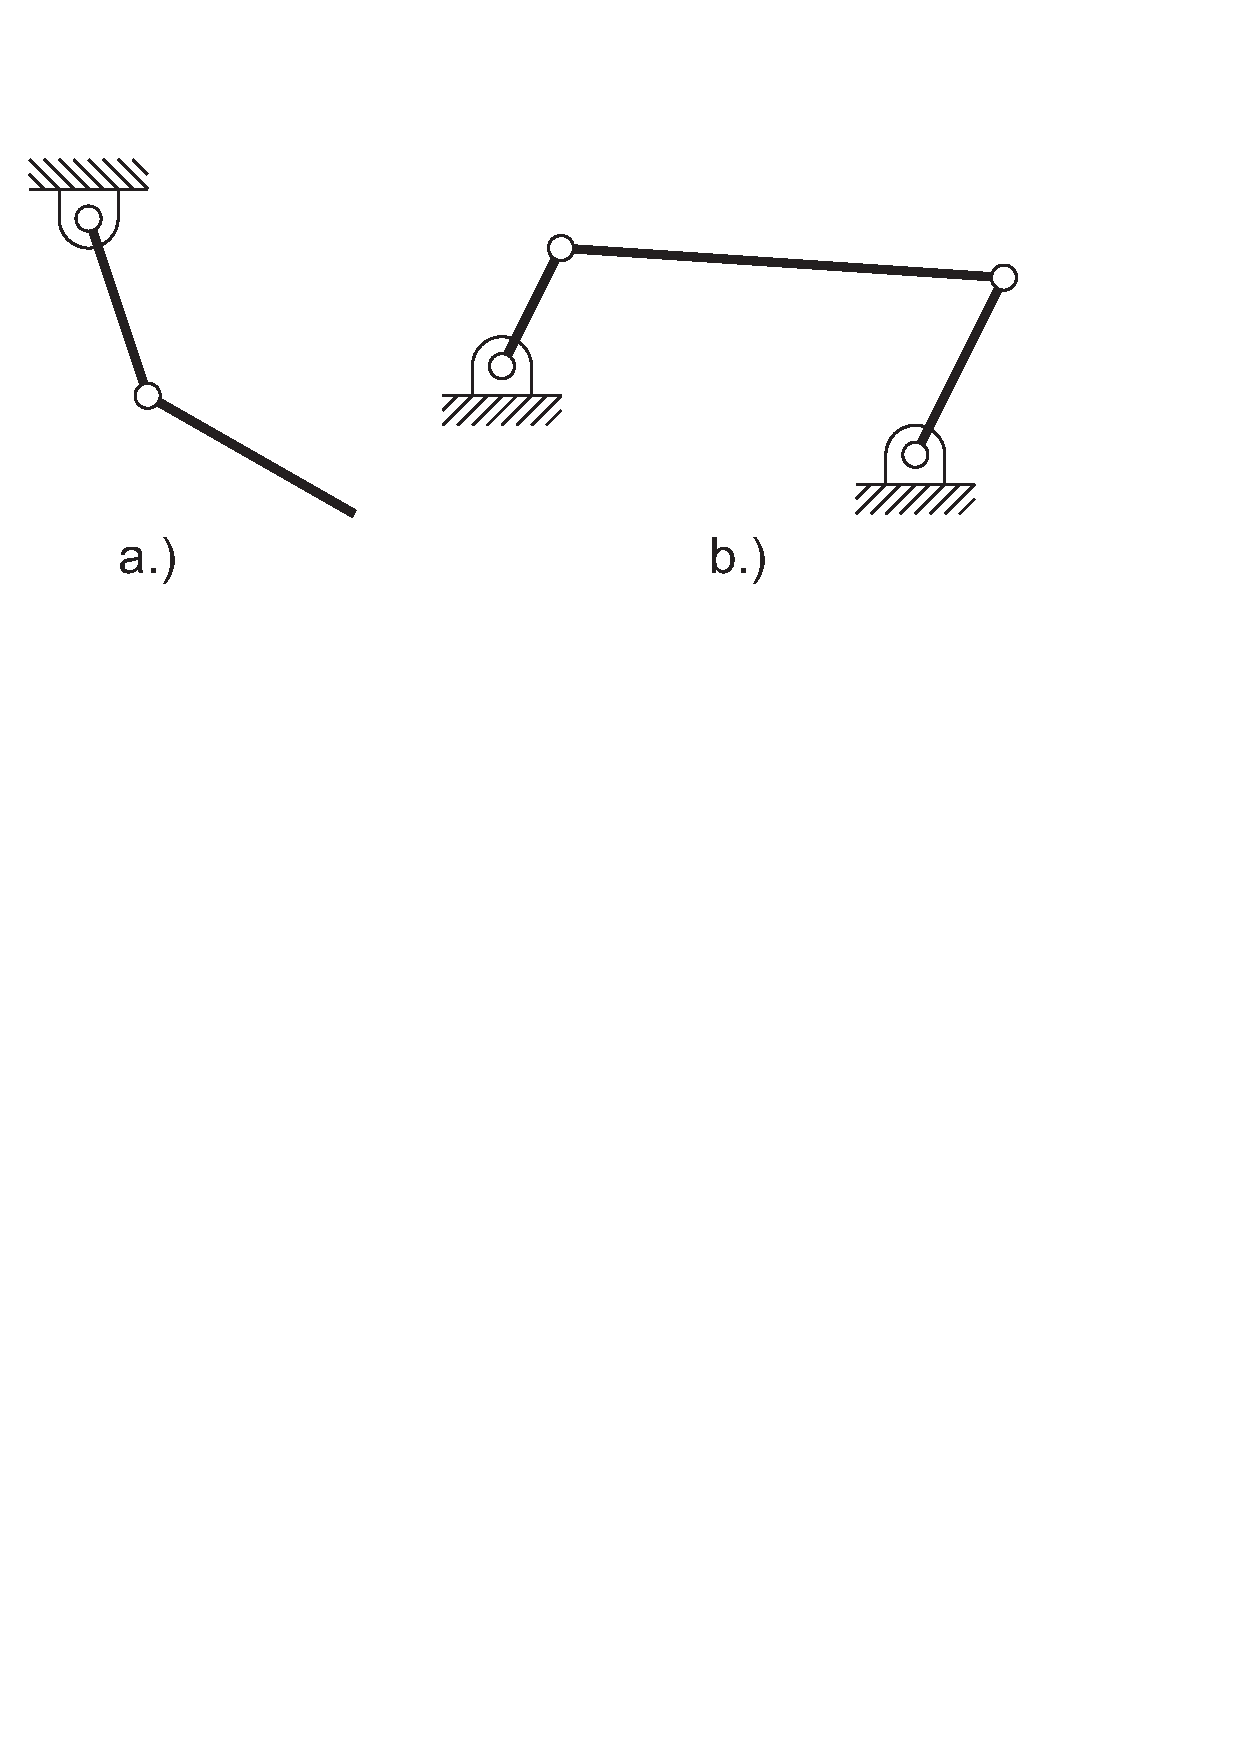
\includegraphics[width=8cm]{figures/open_closed_loop}
%\caption{a.) Open loop mechanism (double pendulum), b.) Closed loops mechanism (four-bar linkage).}
%\label{fig_open_closed_loop}
%\end{center}
%\end{figure}

%+++++++++++++++++++++++++++++++++++++++++++++++++++++++++++++++++++++++++++++++
\mysubsubsubsection{Kinematic pairs}
During early achievements in kinematics, joints have been denoted as kinematic pairs, where the pair represents two bodies where joint constraints are imposed at. There are joints denoted as \mybold{lower pairs}, which are defined by the idealized contact of two rigid surfaces, each of which attached to one of the two bodies. The most prominent types, with mention of the respective object names in \codeName, are:
\bi
  \item spherical joint (S), ball and socket joint; three constraints on relative translation of body-fixed points; \texttt{ObjectJointSpherical}
  \item revolute (R) joint, hinged joint; three spherical joint constraints plus two on tilting around axes normal to the joint axis; \texttt{ObjectJointRevolute}
  \item prismatic (P) joint; tree constraints on relative rotation; \texttt{ObjectJointPrismatic}
  \item screw (helical, H) joint; \texttt{not yet available}
  \item cylindrical (C) joint; \texttt{ObjectJointGeneric}
  \item planar joint; restricts motion to plane, thus adding one relative translation and two rotation constraints; \texttt{ObjectJointGeneric}
\ei
A very practical joint, which has no relevance for kinematics, is the rigid joint (6 constraints, \texttt{ObjectJointGeneric}). It simply constrains the rigid body motion of two bodies, making the two bodies identical from the rigid body kinematics viewpoint.

\mybold{Higher pairs} involve changing surfaces or curves of contact, such as in a cam and follower or gears.

Indeed, some cases in constraints may not be represented by a set of kinematic pairs, such as several mass points arranged along an inextensible string. Therefore, codeName\ usually employs kinematic pairs, but also allows an arbitrary number of bodies to be coupled.

%+++++++++++++++++++++++++++++++++++++++++++++++++++++++++++++++++++++++++++++++
%+++++++++++++++++++++++++++++++++++++++++++++++++++++++++++++++++++++++++++++++
\mysubsubsection{Euler's and Chasles's Theorems}
%this section follows Nikravesh! see also Goldstein
%new: UIBK!

In the following, we consider so-called active rotations of bodies. Consider a body rotating with an angular velocity $\tomega$. Thereing, the orientation of the body can be given with respect a previous orientation using a transformation matrix (rotation matrix).
Here, the components of the transformation matrix are given as a function of time. When reconsidering the \ac{DOF} of a mechanism, it is thus the question, how many independent coordinates are required to describe a spatial rotation?

The answer to this question is given by Euler's theorem:
\bi
  \item \mybold{Euler's theorem}: The general displacement of a body with one point fixed is a rotation about some axis.
\ei
%
The latter theorem states that at any current time $t$ and after any rotations, the orientation of the body can be described by a rotation axis and a single rotation angle. Note that this rotation axis is used to describe the rotation of the body from the initial to the current time at once, although, the rotation might have been performed by means of many different successive rotations. This rotation axis is different from the so-called \mybold{instantaneous axis of rotation} of the body. As a consequence, points lying at the rotation axis are not affected by this rotation.

In addition to Euler's theorem, we mention \mybold{Chasles's theorem}, which reads as follows:
%[Schahl'] %Michel Chasles, Franz., 1793-1880
\bi
  \item \mybold{Chasles's theorem}: The most general displacement of a body is a translation plus a rotation.
\ei
Therefore, the general motion of the rigid body follows from Euler's theorem plus a translation of the point which was originally fixed.

%+++++++++++++++++++++++++++++++++++++++++++++++++++++++++++++++++++++++++++++++
%+++++++++++++++++++++++++++++++++++++++++++++++++++++++++++++++++++++++++++++++
\mysubsubsection{Degree of freedom -- \ac{DOF}}
%definition Nikravesh
According to Nikravesh, "The minimum number of coordinates required to fully describe the configuration of a system
is called the number of degrees of freedom of the system".
We may consider two examples given in \fig{fig_degrees_of_freedom}, to understand the \ac{DOF}.
A double pendulum is shown, which can be described with no less than two independent angles $\phi_1$ and $\phi_2$, thus the system has two degrees of freedom. 

As a second example, a four-bar mechanism is shown, see \fig{fig_degrees_of_freedom}b.
There are three angles $\phi_a$, $\phi_b$ and $\phi_c$ related with the current configuration of the system. 
However, there are two algebraic relations (constraint conditions) between these three angles, given as
\bea
  {l_a\sin(\phi_a) + l_b\sin(\phi_b) - l_c\sin(\phi_c) - d_1 = 0} \nonumber \\
  {l_a\cos(\phi_a) - l_b\cos(\phi_b) - l_c\cos(\phi_c) + h_1 = 0}   
\eea
In the latter two equations, the angles $\phi_a$ and $\phi_b$ can be expressed in terms of $\phi_c$. 
Thus, $\phi_c$ is the only remaining independent (minimum) coordinate of the system, and as a consequence, the system has only one degree of freedom.
Regarding the four-bar mechanism, there exist some configurations, which can lead to bifurcation and a change in the degrees of freedom -- but this is usually avoided in practical cases.
%
\LatexRSTfigure{figures/degrees_of_freedom}{fig_degrees_of_freedom}{10cm}{500}{Examples of mechanisms with different degrees of freedom.}
%\begin{figure}[htb]
%\begin{center}
%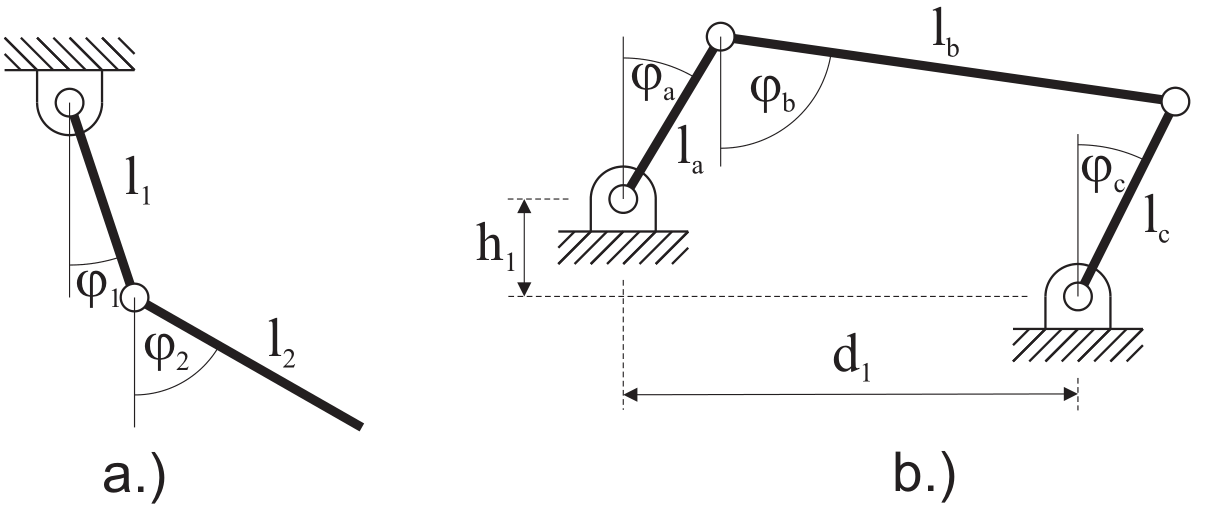
\includegraphics[width=12cm]{figures/degrees_of_freedom}
%\caption{Examples of mechanisms with different degrees of freedom.}
%\label{fig_degrees_of_freedom}
%\end{center}
%\end{figure}

%+++++++++++++++++++++++++++++++++++++++++++++++++++++++++++++++++++++++++++++++
\mysubsubsection{Non-holonomic constraints}
It should be noted, that the above given definition works well with holonomic constraints. In case of non-holonomic systems, the non-holonomic constraints, which may only be given at velocity level, lead to different degrees of freedom on position and velocity level.
Due to the fact that time integration integrates velocities and accelerations, and constraints may be formulated on position or velocity in \codeName, non-holonomic constraints are not largely influencing the structure of the system of equations. However, in view of the constraint jacobian, it usually reflects the constraints on velocity level, as this is the matrix which the incremental solver uses to update coordinates.

%+++++++++++++++++++++++++++++++++++++++++++++++++++++++++++++++++++++++++++++++
\mysubsubsection{Dependent and independent coordinates}
Assuming a holonomic mechanical system with $k$ degrees of freedom, one can find $k$ \mybold{independent} \mybold{coordinates} (\mybold{minimum coordinates}) to completely describe the system configuration. Note that these coordinates do not necessarily have the meaning of displacement, length or angle, but they may be more general (generalized coordinates).

In addition to the independent coordinates, there may be \mybold{dependent coordinates}, similar to the angles $\phi_a$ and $\phi_b$ which are dependent on $\phi_c$ in the example of the four-bar mechanism. It is left to the engineer, whether to find the minimum coordinates of a system and to write all equations in terms of these, or to work with a larger set of independent and dependent coordinates together with algebraic constraint conditions.

%+++++++++++++++++++++++++++++++++++++++++++++++++++++++++++++++++++++++++++++++
\mysubsubsection{Chebychev-Gr\"ubler-Kutzbach criterion}
%Grübler-Kutzbach
A \mybold{rigid body in space has six degrees of freedom}, and thus, six independent coordinates can be used to describe its configuration.
Thus for a system with $n_b$ bodies, there are $6 \cdot n_b$ coordinates, to describe the bodies.
Assuming that there are a set of spheric, revolute, prismatic and other joints, which reduce the degrees of freedom, we denote the number of \mybold{independent constraints} to be of size $n_c$.
It is important, that the constraint equations are (linearly) independent, because in kinematics it is possible to restrict the motion with redundant constraints, see later.

Finally, having $n_b$ rigid bodies $n_c$ scalar, independent constraint equations, the degrees of freedom are given as
\be \label{eq:Chebychev:Grubler:Kutzbach}
  n_\mathrm{DOF} = 6 \cdot n_b - n_c
\ee
which is denoted sometimes as the \mybold{Kutzbach}, or \mybold{Chebychev-Gr\"ubler-Kutzbach criterion}. 

In the case of planar mechanisms, a body obtains only three degrees of freedom. Therefore the Chebychev-Gr\"ubler-Kutzbach criterion reads
\be
  DOF_\mathrm{planar} = 3 \cdot n_b - n_c
\ee

As a spatial example, consider again the double pendulum \fig{fig_degrees_of_freedom}a as a spatial mechanism.
In this case, there are two bodies, $n_b=2$ and two revolute joints with 5 constraints each, giving $n_c=10$. Thus, the Chebychev-Gr\"ubler-Kutzbach criterion gives $n_\mathrm{DOF} = 12 - 10 = 2$, which we expect.

As another example, consider a spatial four-bar mechanism according to \fig{fig_degrees_of_freedom}b.
In this case, there are four bodies, $n_b=4$, four revolute joints with 5 constraints each and a ground joints with 6 constraints, totalling at $n_c=4\cdot 5 + 6 = 26$. Thus, \eq{eq:Chebychev:Grubler:Kutzbach} gives 
\be
  n_\mathrm{DOF} = 24 - 26 = -2.
\ee
This is certainly not what we expect, as we know that the mechanism can move and has $n_\mathrm{DOF} = 1$. The reason for this number lies in redundant constraints, which may not be counted for the Chebychev-Gr\"ubler-Kutzbach criterion.
A solution to this problem is to replace one revolute joint by a planar revolute joint (2 constraints), which then gives
\be
  n_c=3\cdot 5 + 2 + 6 = 23 \quad \mathrm{and} \quad n_\mathrm{DOF} = 1.
\ee
Therefore, \codeName uses an \mybold{extended Chebychev-Gr\"ubler-Kutzbach criterion} for redundant constraints,
\be \label{eq:Chebychev:Grubler:Kutzbach:ext}
  n_\mathrm{DOF}^* = n_\mathrm{ODE2} - (n_c - n_{ca} - n_r)
\ee
where $n_r$ is the number of redundant constraints and $n_\mathrm{ODE2}$ is the number of \ac{ODE2} coordinates, which may be $6 \cdot n_b$ for purely spatial rigid bodies, $n_{ca}$ are pure algebraic constraints and $n_r$ are redundant constraints.

In \codeName, there is a function \texttt{ComputeSystemDegreeOfFreedom} in the \texttt{solver} module, available as
\bi
  \item[] \texttt{mbs.ComputeSystemDegreeOfFreedom(verbose=True)}
\ei
which allows to compute \ac{ODE2} coordinates ($=n_\mathrm{ODE2}$), total constraints ($=n_c$), redundant constraints ($=n_r$), and the degree of freedom ($=n_\mathrm{DOF}^*$). In addition, the function also computes the number of pure algebraic constraints ($=n_{ca}$), which are internal constraints, which only act on the algebraic quantities but do not affect \ac{ODE2} coordinates. 
As an example for pure algebraic constraints, in a \texttt{GenericJoint} inactive constraints are replaced by $\lambda_i=0$ ($\lambda$ being the Lagrange multiplier), thus reducing the number of effective constraints in the system.
%


%+++++++++++++++++++++++++++++++++++++++++++++++++++++++++++++++++++++++++++++++
%+++++++++++++++++++++++++++++++++++++++++++++++++++++++++++++++++++++++++++++++
\mysubsubsectionlabel{Generalized coordinates}{sec:theory:generalized:coordinates}
 
In \mybold{Cartesian coordinates}, three parameters (denoted as coordinates) are used to uniquely define the position of any point with respect to a Cartesian coordinate system.
The position and orientation of a rigid body can be uniquely defined by means of three position and three rotation parameters (rigid body coordinates).

The position and orientation as well as the deformation in deformable bodies can be defined by a \mybold{set of coordinates}. We require that any set of coordinates uniquely defines the position of all points of the bodies.
As the bodies move, the coordinates vary with time.
The set of $n$ generalized coordinates is commonly represented by a (column) vector
\be
  \qv = [q_0, q_1, \ldots, q_{n-1}]\tp,
\ee
in which $n$ represents the total number of coordinates that are used. 
In \codeName, position, orientation and deformation coordinates (of bodies) are denoted as \ac{ODE2} coordinates, as they are related to second order differential equations, the main criterion to distinguish computational coordinates in the system.

The \mybold{generalized (Lagrangian) coordinates}, which are employed in Lagrange's equations of motion, are another set of well known coordinates used for mechanisms. As known from Lagrange's formalism, coordinates may be defined relative to each other.

\mysubsubsection{Reference and current coordinates}
%
An important fact on the coordinates used in \codeName is upon the \mybold{additive}\footnote{This additive splitting is also used for rotations: therefore, only the sum of reference and current (or visualization) coordinates has a geometrical meaning, while the parts are only used within the solver for incrementing.} splitting of quantities (e.g. position, rotation parameters, etc.) into \mybold{reference} and \mybold{current} (initial/visualization/...) coordinates.
The current position vector of a point node is computed from the reference position plus the current displacement, reading
\be
  \pv\cCur = \pv\cRef + \uv\cCur
\ee
In the same way rotation parameters are computed from,
\be
  \ttheta\cCur = \ttheta\cRef + \tpsi\cCur
\ee
which are based on reference quantities plus displacements or changes. Note that these changes are additive, even for rotation parameters. Needless to say, $\tpsi\cCur$ do not represent rotation parameters, while $\ttheta\cRef$ should be chosen such that they represent the orientation of a node in reference configuration.
The necessity for reference coordinates originates from finite elements, which usually split nodal position into displacements and reference position.
However, we also use the reference position here in order to define joints, e.g., using the utility function \texttt{CreateRevoluteJoint(...)}.

Note that this splitting is only employed for position coordinates, but not for displacements or velocities!

%+++++++++++++++++++++++++++++++++++++++++++++++++++++++++++++++++++++++++++++++
%+++++++++++++++++++++++++++++++++++++++++++++++++++++++++++++++++++++++++++++++
\mysubsection{Dynamics: Mechanical principles}
Following kinematics, dynamics comes into play, which involves the study of the forces and torques that cause the motion, bridging the gap between the motion observed and the reasons behind it.
In this section, we shortly recap mechanical principles, which are used throughout for the simulation of multibody systems.

%+++++++++++++++++++++++++++++++++++++++++++++++++++++++++++++++++++++++++++++++
%+++++++++++++++++++++++++++++++++++++++++++++++++++++++++++++++++++++++++++++++
\mysubsubsection{Newton's basic principles}
In the study of multibody systems, Newton's basic principles lay the foundational framework. At the heart of these principles are three laws that govern the motion of bodies:

\noindent \mybold{1. Newton's first law (law of inertia)}: A body remains at rest, or in uniform motion in a straight line, unless acted upon by a force $\fv$, expressed as:
\be
  \fv = 0 \implies \frac{\dd \vv}{\dd t} = 0
\ee
where $\fv$ is the net force applied to the body, and $\frac{d\vv}{dt}$ is the acceleration of the body.

\noindent\mybold{2. Newton's second law (law of motion)}: The sum of the forces F acting on a point mass equals the change in momentum of this mass, 
\be
  \fv= \frac{\dd\,\Jm}{\dd t} = \dot \Jm 
\ee
where $\Jm$ is the (linear, translational) momentum of the mass $m$. Assuming a constant mass of the body (which is not true for some cases such as rockets), we find that the acceleration $\av$ of an object is directly proportional to the net force $\fv$ acting upon it and inversely proportional to its mass, given by the equation:
\be \label{eq:theory:newton:fma}
  \fv= m \av
\ee
where $m$ is the mass of the object.
  
\noindent \mybold{3. Newton's third law (action and reaction)}: For every action, there is an equal and opposite reaction. This principle is fundamental in analyzing the interactions within multibody systems and can be summarized as:
\be
  \fv_{12} = -\fv_{21}
\ee
in which we observe $\fv_{12}$ as the force exerted by body 1 on body 2, and $\fv_{21}$ as the force exerted by body 2 on body 1.

These principles are pivotal in understanding and modeling the dynamics of multibody systems, providing the basis for further exploration and analysis in this field.
Newton's principles represent linear (translational) motion, but may be transformed to rotations by using angular momentum, as well. This leads to Euler's equations, see the description of the \texttt{ObjectRigidBody}.

%+++++++++++++++++++++++++++++++++++++++++++++++++++++++++++++++++++++++++++++++
%+++++++++++++++++++++++++++++++++++++++++++++++++++++++++++++++++++++++++++++++
\mysubsubsection{The Lagrange-d'Alembert principle}
%
For a constant mass $m$, it follows from Newton's second law that
\be \label{eq_newton_dalembert}
  \sum \fv  = m \av \eqComma
\ee
\eq{eq_newton_dalembert} can also be written in the form
\be
  \sum \fv - m \av = \Null
\ee
The vector $(- m \av )$ is referred to as the inertia force, since it can apparently be balanced to zero in the sense of a generalized equilibrium. This equilibrium is called dynamic equilibrium, in analogy to statics.

In \mybold{D'Alembert's Principle}, the inertia force $\fv_i = -m \av$ is introduced, and the sum of the forces is written as
\be
  \fv_e + \fv_c + \fv_i = \mathbf{0}
\ee
where applied forces $\fv_e$ and constraint forces $\fv_c$ are distinguished.

A key property of the constraint forces is that the virtual work done by constraint forces always vanishes,
\be \label{eq_virt_arb_zwangskraefte}
  \fv_c \cdot \delta \rv = 0 \eqDot
\ee
where here $\delta \rv$ is the virtual displacement associated with the constraint force.

%+++++++++++++++++++++++++++++++++++++++++++++++++++++++++++++++++++++++++++++++
\mysubsubsection{Generalized Principle of Virtual Work}
%
With the generalized principle of virtual work, it follows
\be
  \left(\fv_e + \fv_i \right) \cdot \delta \rv = 0 \quad \text{or} \quad
\ee
Thus, we obtain the \mybold{Lagrange-d'Alembert} principle as
\be
  \delta W_e + \delta W_T = 0 \quad \text{or} \quad
\ee
with the virtual work $W_e$ of applied forces and $W_i$ of inertia forces,
\be
  \delta W_e = \fv_e \cdot \delta \rv \quad \mathrm{and} \quad
  \delta W_T = \fv_i \cdot \delta \rv \eqDot
\ee
For a system of $n$ mass points, it follows
\be
  \sum_{i=0}^{n-1} \left(\fv_{e,i} \cdot \delta \rv_i -  m_i \av_i \cdot \delta \rv_i \right) = 0
\ee
It is ultimately characterized by the fact that, in comparison to D'Alembert's principle, constraint forces do not appear.

Note that this principle is used in \codeName at many places to derive equations for rigid and flexible bodies, as well as for connectors, such as spring-dampers.

%+++++++++++++++++++++++++++++++++++++++++++++++++++++++++++++++++++++++++++++++
\mysubsubsection{Virtual displacements}
The virtual displacement $\delta \rv_j$ or the variation of any quantity can be written in terms of variation of the underlying coordinates, see \refSection{sec:theory:generalized:coordinates},
\be\label{eq:theory:virtual:displacement}
  \delta \rv_j = \sum_{i=1}^n \frac{\partial \rv_j}{\partial  q_i} \delta q_i \eqDot
\ee

%+++++++++++++++++++++++++++++++++++++++++++++++++++++++++++++++++++++++++++++++
\mysubsubsection{Generalized Forces}
To derive the Lagrangian equations, we first consider the virtual work done by $N$ forces on $N$ mass points
\be
  \delta W = \sum_{j=1}^N \fv_j \cdot \delta \rv_j \eqDot
\ee
Here, $\fv_j$ represents the force on, and $\delta \rv_j$ represents the displacement of, the $j$th mass point.

Using \eq{eq:theory:virtual:displacement}, the virtual work can be expressed as
\be
  \delta W = \sum_{j=1}^N \fv_j \cdot \sum_{i=1}^n \frac{\partial \rv_j}{\partial  q_i} \delta q_i = 
  \sum_{i=1}^n \left(\sum_{j=1}^N \fv_j \cdot \frac{\partial \rv_j}{\partial  q_i} \right) \delta q_i \eqDot
\ee
%
In the process of translating the virtual work of forces or moments, we identify what are called generalized forces $Q_i$,
\be\label{eq:theory:generalized:forces}
  Q_i = \sum_{j=1}^N \fv_j \cdot \frac{\partial \rv_j}{\partial  q_i} \eqDot 
\ee
Consequently, the virtual work can also be written as,
\be
  \delta W = \sum_{i=1}^n Q_i \, \delta q_i \eqDot
\ee


%+++++++++++++++++++++++++++++++++++++++++++++++++++++++++++++++++++++++++++++++
%+++++++++++++++++++++++++++++++++++++++++++++++++++++++++++++++++++++++++++++++
\mysubsubsection{Lagrange's Equations of Motion}
%
We define the kinetic energy as $T$, which for $N$ mass points is given by
\be
  T = \frac{1}{2} \sum_{j=1}^N  m_j \vv_j^2
\ee
Using the kinetic energy $T$, the following \mybold{Lagrangian equations} can be written,
\be
  \frac{\mathrm{d}}{\mathrm{d}t} \frac{\partial T}{\partial \dot q_i} - \frac{\partial T}{\partial q_i} = Q_i, \quad i=1,2,\ldots,n \eqDot
\ee
These are valid under the assumption of minimal coordinates with holonomic constraints, resulting in the fact that all virtual displacements $\delta q_i$ are independent of each other.

For forces that possess a potential $V$, i.e. the variation of the potential reads
\be
  \delta V = \sum_{i=1}^n \frac{\partial V}{\partial q_i}\delta q_i = - \sum_{i=1}^n Q_i^{(V)} \delta q_i \eqComma
\ee
and assuming that $Q_i$ now only includes forces \mybold{without a potential}, the Lagrange equations can be rewritten as follows,
\be
  \frac{\mathrm{d}}{\mathrm{d}t} \frac{\partial T}{\partial \dot q_i} - \frac{\partial T}{\partial q_i} = Q_i + Q_i^{(V)}=
  Q_i - \frac{\partial V}{\partial q_i}, \quad i=1,2,\ldots,n \eqDot
\ee
With the \mybold{definition} $L=T-V$ and the relationship $\frac{\partial V}{\partial \dot q_i} = 0$, a common form of Lagrange's equations is obtained:
\be
  \frac{\mathrm{d}}{\mathrm{d}t} \frac{\partial L}{\partial \dot q_i} - \frac{\partial L}{\partial q_i} = Q_i, \quad i=1,2,\ldots,n \eqDot
\ee
This equation is also used sometimes to derive equations of motion for rigid or flexible bodies in \codeName.

%+++++++++++++++++++++++++++++++++++++++++++++++++++++++++++++++++++++++++++++++
%+++++++++++++++++++++++++++++++++++++++++++++++++++++++++++++++++++++++++++++++
\mysubsubsection{Multibody formulations: redundant and minimal coordinates}
%
In multibody system dynamics, we primarily distinguish between two formulations:
\bi
  \item \mybold{redundant coordinates}
  \item \mybold{minimal coordinates}
\ei
Formulations based on minimal coordinates appeared naturally and early, in principle every model in dynamics, 
such as a 1D motion of a mass point according to Newton's laws, see \eq{eq:theory:newton:fma}, Euler's equations, or a single DOF mass-spring-damper model. 
The \mybold{advantages of a minimal-coordinates} formulation are:
\bi
  \item coordinates represent the degrees of freedom
  \item direct access to relevant coordinates
  \item direct application of forces to the coordinates
  \item application of any class of solvers, as long as equations are non-stiff
\ei
The \mybold{disadvantages} are related to the \mybold{additional efforts to derive the equations of motion}, which has to be done for every different system,
and the general restriction to open-loop systems, making it difficult to be applied to closed-loop systems (but not always impossible). 
There are many modifications, which allow closed-loop systems, e.g., via augmented Lagrangians or similar approaches.

\noindent A \mybold{redundant-coordinates} formulation has the following \mybold{advantages}:
\bi
  \item being \mybold{extremely versatile} and allowing practically any combination of (closed-loop) constraints
  \item easy extension to flexible bodies, sliding constraints, etc.
  \item multibody systems can be created easily by \mybold{combining a set of bodies and constraints} ($\ra$ user friendly)
\ei
\mybold{Disadvantages} are clearly the \mybold{resulting index 3} (position-level) constraints, 
for which only very few implicit solvers (time integration) exist, and it requires always matrix factorization during solving.
A further problem is that this formulation may potentially lead to redundant constraints, which need to be treated specially with solvers,
and that the degrees of freedom are less obvious and that relevant \mybold{(e.g., joint) coordinates are not directly accessible} on the equations level.

\noindent It is left to the user, which formulation to chose when working with multibody systems. 
In \codeName, there is the option to create tree-like rigid body systems
using the \texttt{ObjectKinematicTree}, which allows to use minimal coordinates for open-loop systems. In general, \codeName is a redundant 
multibody dynamics formulation for reasons of simpler assembly of equations of motion.

\noindent As an example, we investigate the equations of motion for a \mybold{mathematical pendulum} with mass $m$, distance $L$ between support and mass,
under gravity $g$.

\noindent In the minimal coordinates formulation, see \fig{fig:theory:formulations:pendulum}, we define the angle $\varphi$, being zero in the horizontal configuration,
\be
  m L \ddot \varphi = m g \cos \varphi
\ee
leading to one $2^\mathrm{nd}$ order ordinary differential equation (ODE2), using the minimal coordinate $\varphi$.
\LatexRSTfigure{figures/pendulum}{fig:theory:formulations:pendulum}{4.5cm}{200}{Mathematical pendulum with minimal coordinate $\varphi$.}

\noindent With redundant coordinates, see \fig{fig:theory:formulations:pendulumConstraint}, we may introduce two Cartesian coordinates ($x$, $y$), to define the location of the mass in 
the plane, leading to two differential equations for the mass point,
\be \label{eq:theory:pendulum:redundantCoords}
  m \ddot x = f_x, \quad
  m \ddot y = f_y
\ee
together with a constraint equation 
\be \label{eq:theory:pendulum:redundantConstraint}
	c(x,y) = \sqrt{x^2 + y^2} - L = 0
\ee
\LatexRSTfigure{figures/pendulumConstraint}{fig:theory:formulations:pendulumConstraint}{4.5cm}{200}{Mathematical pendulum with redundant coordinates ($x$, $y$).}

\noindent Note that \eq{eq:theory:pendulum:redundantCoords} and \eq{eq:theory:pendulum:redundantConstraint} include 3 equations for only two unknowns ($x$, $y$). 
Therefore, we need to introduce an additional unknown Lagrange multiplier $\lambda$ for the redundant multibody formulation,
which represents a force in direction of the pendulum's string, exactly such that the length $L$ is preserved.
The factor $\lambda$ has to be projected with the constraint derivatives (Jacobian) onto the coordinates ($x$, $y$), giving the forces
\be
  f_x = -\frac{\partial c}{\partial x} \lambda, \quad
  f_y = m g - \frac{\partial c}{\partial y} \lambda \eqDot
\ee
Therefore, we can rewrite \eq{eq:theory:pendulum:redundantCoords} as
\be \label{eq:theory:pendulum:redundantFinal}
  m \ddot x + \frac{\partial c}{\partial x} \lambda = 0, \quad
  m \ddot y + \frac{\partial c}{\partial y} \lambda = m g
\ee
with the algebraic constraint, written in a computationally more efficient form,
\be \label{eq:theory:pendulum:redundantConstraintFinal}
  c(x,y) = x^2 + y^2 - L^2 = 0
\ee
The equations of motion are formed by both \eq{eq:theory:pendulum:redundantFinal} and \eq{eq:theory:pendulum:redundantConstraintFinal},
which are \mybold{differential-algebraic equations (DAEs) of index 3} and therefore much harder to solve than ordinary differential equations
in case of minimal coordinates.

\noindent In \codeName, we therefore use either the generalized-$\alpha$ solver, or an implicit trapezoidal rule in combination with an index 2
reduction, see the section on solvers for more details.

%+++++++++++++++++++++++++++++++++++++++++++++++++++++++++++++++++++++++++++++++
%+++++++++++++++++++++++++++++++++++++++++++++++++++++++++++++++++++++++++++++++
\mysubsection{Frames, rotations and coordinate systems}
In this section, we introduce frames, which provide reference points and rotations attached to the ground or to bodies, thus providing a bases for coordinate systems.

%+++++++++++++++++++++++++++++++++++++++++++++++++++++++++++++++++++++++++++++++++++++++++++
%+++++++++++++++++++++++++++++++++++++++++++++++++++++++++++++++++++++++++++++++++++++++++++
\mysubsubsection{Reference points and reference frames}
%
In contrast to the reference coordinates (which may include reference position and rotations), the reference point of a body, marker or joint is available in any configuration (current, initial, etc.). 
The reference point and orientation (or reference frame) of a rigid body coincides with the position and orientation of the underlying node.
The local position of a point of the body is expressed relative to the body's reference frame, which may be different from the body's center of mass.
%
The reference frame is also used for \hac{FFRF} objects. In most cases, reference points are denoted by $\pRef$.

%+++++++++++++++++++++++++++++++++++++++++++++++++++++++++++++++++++++++++++++++++++++++++++
\mysubsubsection{Coordinate systems of frames}
%
Many considerations and computations in kinematics can be formulated coordinate-free.
However, ultimately local positions are given by the user in different coordinates from results given in global (world) coordinates.

For this reason, we use left upper indices in symbols to indicate underlying frames of points or vectors, e.g.,
$\LU{0}{\uv}$ represents a displacement vector in the global (world) coordinate system $0$, while 
$\LU{m1}{\uv}$ represents the displacement vector in marker 1 ($m1$) coordinates. 

Typical coordinate systems (frames) are:
\bi
  \item $\LU{0}{\uv}$ $\ldots$ global or world coordinates
  \item $\LU{b}{\uv}$ $\ldots$ body-fixed, local coordinates
  \item $\LU{m0}{\uv}$ $\ldots$ local coordinates of (the body or node of) marker $m0$
  \item $\LU{m1}{\uv}$ $\ldots$ local coordinates of (the body or node of) marker $m1$
  \item $\LU{J0}{\uv}$ $\ldots$ local coordinates of joint $0$, related to marker $m0$
  \item $\LU{J1}{\uv}$ $\ldots$ local coordinates of joint $1$, related to marker $m1$
\ei
To transform the local coordinates $\LU{m0}{\uv}$ of marker 0 into global coordinates $\LU{0}{\xv}$, we use the relation
\be \label{eq:theory:coordinateSystems:rot}
  \LU{0}{\uv} = \LU{0,m0}{\Rot} \LU{m0}{\uv}
\ee
in which $\LU{0,m0}{\Rot}$ is the transformation matrix of (the body or node of) the underlying marker 0.

In particular, note that any transformation, e.g., of the angular velocity in body (b) and world coordinates,
\be
  \LU{0}{\tomega} = \LU{0,b}{\Rot} \LU{b}{\tomega}
\ee
only transforms the vector from one frame to the other, but does not change the vector $\tomega$ itself.



%+++++++++++++++++++++++++++++++++++++++++++++++++++++++++++++++++++++++++++++++
%+++++++++++++++++++++++++++++++++++++++++++++++++++++++++++++++++++++++++++++++
\mysubsubsection{Homogeneous transformations}
%basic formula
%check if exists in theDoc
%HT: refer to this section
In order to considere rotations and translations in frames, homogeneous transformations are used.
An arbitrary vector $\LU{i}{\rv}$ in coordinates of frame $\mathcal{F}_i$ can be expressed relative to $\mathcal{F}_j$ with the vector $\LU{j}{\pv_i}$, pointing from $O_j$ to $O_i$ and a rotation matrix according to \eq{eq:theory:coordinateSystems:rot}:
\be \label{eq:theory:HT:positionRelation}
  \LU{j}{\rv} = \LU{ji}{\Rm} \LU{i}{\rv} + \LU{j}{\pv_i}
\ee
\eq{eq:theory:HT:positionRelation} can be written as a linear mapping,
\be
  \vp{\LU{j}{\rv}}{1} = \mp{\LU{ji}{\Rm}}{\LU{j}{\pv_i}}{\Null^T}{1} \vp{\LU{i}{\rv}}{1}, \quad
\ee
in which the matrix
\be
  \LU{ji}{\Tm} = \mp{\LU{ji}{\Rm}}{\LU{j}{\pv_i}}{\Null^T}{1} 
\ee
is referred to as the \mybold{homogeneous transformation matrix}, and $\LU{j}{\hat \rv} = [\LU{j}{\rv} \;\; 1]^T$ is the homogeneous vector corresponding to $\LU{j}{\rv}$.

Analogous to the rotation matrix, $\LU{ji}{\Tm}$ has an inverse, which follows as
\be
  \LURU{ji}{\Tm}{}{-1} = \LU{ij}{\Tm} = \mp{\LURU{ji}{\Rm}{}{T}} {-\LURU{ji}{\Rm}{}{T} \LU{j}{\pv_i}}{\Null^T}{1} \vp{\LU{j}{\rv}}{1} \eqDot
\ee
Sequential application of homogeneous transformations simplifies to
\be
  \LU{ki}{\Tm} = \LU{kj}{\Tm} \LU{ji}{\Tm} \eqDot
\ee
We could also actively move vectors, by assuming that the homogeneous transformation matrix $\LU{i0,i1}{\Tm}$ transforms coordinates within the same frame $\mathcal{F}_i$, between two (time) steps 0 and 1,
\be
  \LU{i1}{\hat \rv} = \LU{i1,i0}{\Tm} \LU{i0}{\hat \rv}
\ee
which advances the vector $\LU{i0}{\hat \rv}$ in time.

Note that an efficient implementation would only include $\Rm$ and $\pv$, without necessarily computing $4 \times 4$ matrices.

%+++++++++++++++++++++++++++++++++++++++++++++++++++++
\onlyRST{

.. _fig-theory-HT-changeOfFrame:
.. figure:: docs/theDoc/figures/theoryRotationsHTchangeOfFrame.png
   :width: 320

   Homogeneous transformation from $\mathcal{F}_i$ to $\mathcal{F}_j$ using the relation $\LU{j}{\hat{\mathbf{r}} } = \LU{ji}{\Tm} \LU{i}{\hat{\mathbf{r}} }$

}
\ignoreRST{
\begin{figure}[tbph]
\begin{center}
\tdplotsetmaincoords{70}{110}
\begin{tikzpicture}[tdplot_main_coords, scale=3]
\draw[thick,->] (0,0,0) -- (1,0,0) node[anchor=north east]{$\ev_{x,i}$};
\draw[thick,->] (0,0,0) -- (0,1,0) node[anchor=north west]{$\ev_{y,i}$};
\draw[thick,->] (0,0,0) -- (0,0,1) node[anchor=south]{$\ev_{z,i}$};

\tdplotsetrotatedcoords{\angA}{\angB}{\angC}
\coordinate (OO) at (-0.1,0.1, 0.6);
\tdplotsetrotatedcoordsorigin{(OO)}
\draw[thick,color=blue!70,tdplot_rotated_coords,->] (0,0,0) --
(1,0,0) node[anchor=north]{$\ev_{x,j}$};
\draw[thick,color=blue!70,tdplot_rotated_coords,->] (0,0,0) --
(0,1,0) node[anchor=west]{$\ev_{y,j}$};
\draw[thick,color=blue!70,tdplot_rotated_coords,->] (0,0,0) --
(0,0,1) node[anchor=south]{$\ev_{z,j}$};
%axis extension
\draw[thick,dashed, color=blue!70,tdplot_rotated_coords] (0,0,0) --
(0,-0.1,0) ;


\coordinate (O) at (0,0,0);
\tdplotsetcoord{P}{1.2}{50}{70};
\sphToCart{1.2}{70}{50}
\pgfmathsetmacro{\xx}{\x+0.1}
\pgfmathsetmacro{\yy}{\y-0.1}
\pgfmathsetmacro{\zz}{\z-0.6}
\tdplottransformmainrot{\xx}{\yy}{\zz}
%\coordinate (Ps) at (\tdplotresx, \tdplotresy, \tdplotresz);
\draw[color=blue!70,tdplot_rotated_coords,dashed] (\tdplotresx,0,0) --(\tdplotresx, \tdplotresy,0);
\draw[color=blue!70,tdplot_rotated_coords,dashed] (0,\tdplotresy,0) --(\tdplotresx, \tdplotresy,0);
\draw[color=blue!70,tdplot_rotated_coords,dashed] (\tdplotresx, \tdplotresy,0) -- (\tdplotresx,\tdplotresy,\tdplotresz);

\draw[color=blue!70,tdplot_rotated_coords,->] (OO)node[anchor=west]{$\mathcal{F}_j$} -- (\tdplotresx,\tdplotresy,\tdplotresz)node[anchor=south]{$\LU{j}{\rv}$};


\draw[->](O)node[anchor=south east]{$\mathcal{F}_i$} --node[anchor=west ]{$\LU{j}{\pv}_i$}(OO);

%draw a vector from origin to point (P)
\draw[ thick, -stealth,color=red!70] (O) -- (P)node[anchor=west]{$\LU{i}{\rv}$};

\draw[dashed] (Px) -- (Pxy);
\draw[dashed] (Py) -- (Pxy);
\draw[dashed] (Pxy) -- (P);

\end{tikzpicture}
\end{center}
\caption{Homogeneous transformation from $\mathcal{F}_i$ to $\mathcal{F}_j$ using the relation $\LU{j}{\hat \rv} = \LU{ji}{\Tm} \LU{i}{\hat \rv}$ .}%
\label{fig:theory:HT:changeOfFrame}%
\end{figure}
}
%+++++++++++++++++++++++++++++++++++++++++++++++++++++

All homogeneous transformations form the \mybold{Special Euclidean Group SE(3)} -- the motion group -- for describing rigid body movements in 3D. Therefore, homogeneous transformations also meet the criteria for groups (closure, associativity, existence of neutral and inverse elements).

Elementary rotations about the $\ev_z$-axis and translations along the $\ev_x$-axis, for example, are given by:
\onlyRST{
\be
  \mathbf{Rot}(\ev_z, \theta) = \vfour{\cos \theta ,\; -\sin \theta ,\; 0 ,\; 0}{\sin \theta ,\; \cos \theta ,\; 0 ,\; 0}{0 ,\; 0 ,\; 1 ,\; 0}{0 ,\; 0 ,\; 0 ,\; 1}, \quad
  \mathbf{Trans}(\ev_x, d) = \vfour{1 ,\; 0 ,\; 0 ,\; d}{0 ,\; 1 ,\; 0 ,\; 0}{0 ,\; 0 ,\; 1 ,\; 0}{0 ,\; 0 ,\; 0 ,\; 1}
\ee
}
\ignoreRST{
\be
  \mathbf{Rot}(\ev_z, \theta) = \mfour{\cos \theta & -\sin \theta & 0 & 0}{\sin \theta & \cos \theta & 0 & 0}{0 & 0 & 1 & 0}{0 & 0 & 0 & 1}, \quad
  \mathbf{Trans}(\ev_x, d) = \mfour{1 & 0 & 0 & d}{0 & 1 & 0 & 0}{0 & 0 & 1 & 0}{0 & 0 & 0 & 1}
\ee
}
Arbitrary composite transformations can be constructed from elementary transformations. In general, the following applies:
\bi
  \item Pre-multiplication (\mybold{Pre-Multiplication}): Transformation in the global coordinate system
  \item Post-multiplication (\mybold{Post-Multiplication}): Transformation in the rotated coordinate system
\ei
By exploiting the tools of so-called Lie groups, rigid body movements can be interpolated using matrix logarithm (\texttt{LogSE3(...)}) and matrix exponential function (\texttt{ExpSE3(...)}).



%+++++++++++++++++++++++++++++++++++++++++++++++++++++++++++++++++++++++++++++++
%+++++++++++++++++++++++++++++++++++++++++++++++++++++++++++++++++++++++++++++++
\mysubsubsection{Rotations}
%basic notation (merge with existing)
%subsequent rotations (figure MKS2023)
%active-passive rotations
%linearized rotations

In this section, we discuss in particular rotations, as already introduced for coordinate systems and homogeneous transformations.
Rotations can be represented by transformation matrices, leading to a linear transformation
\be
   \LU{0}{\rv} = \LU{0,1}{\Rot} \LU{1}{\rv}
\ee
which transforms the vector $\LU{1}{\rv}$ accordingly.
However, rotations are inherently nonlinear. First, rotation parametrizations -- except for the components of the rotation matrix itself -- are highly nonlinear functions of rotation parameters.
Second, subsequent rotations couple in a multiplicative (i.e., nonlinear) way. Therefore rotations have to be treated differently from translations.


%+++++++++++++++++++++++++++++++++++++++++++++++++++++++++++++++++++++++++++++++
\mysubsubsubsection{Derivation of the transformation matrix from coordinate transformations}

The vector $\av$ can be represented in coordinates of frame $\mathcal{F}_1$ with basis vectors $(\ev_{x1},\,\ev_{y1},\,\ev_{z1})$ and of frame $\mathcal{F}_2$ with basis vectors $(\ev_{x2},\,\ev_{y2},\,\ev_{z2})$,
\be \label{eq:theory:rotations:trans1}
  \av = \LUR{1}{a}{x} \ev_{x1} + \LUR{1}{a}{y} \ev_{y1} +\LUR{1}{a}{z} \ev_{z1} =       
        \LUR{2}{a}{x} \ev_{x2} + \LUR{2}{a}{y} \ev_{y2} +\LUR{2}{a}{z} \ev_{z2} \eqDot
\ee
Multiplying \eq{eq:theory:rotations:trans1} with the basis vectors $(\ev_{x1},\,\ev_{y1},\,\ev_{z1})$ consecutively, we obtain three relations,
\bea
  \LUR{1}{a}{x} &=& \LUR{2}{a}{x} \ev_{x1}^T\ev_{x2} + \LUR{2}{a}{y} \ev_{x1}^T\ev_{y2} +\LUR{2}{a}{z} \ev_{x1}^T\ev_{z2} \eqComma \nonumber\\
  \LUR{1}{a}{y} &=& \LUR{2}{a}{x} \ev_{y1}^T\ev_{x2} + \LUR{2}{a}{y} \ev_{y1}^T\ev_{y2} +\LUR{2}{a}{z} \ev_{y1}^T\ev_{z2} \eqComma \nonumber\\
  \LUR{1}{a}{z} &=& \LUR{2}{a}{x} \ev_{z1}^T\ev_{x2} + \LUR{2}{a}{y} \ev_{z1}^T\ev_{y2} +\LUR{2}{a}{z} \ev_{z1}^T\ev_{z2} \eqDot
\eea
where we apply the orthonormality relationships $\ev^T_{x1} \ev_{x1} = 1$, $\ldots$ as well as $\ev^T_{x1} \ev_{y1} = 0$, $\ev^T_{x1} \ev_{z1} = 0$, $\ldots$ througout.

We can represent the result as linear transformation
\be
  \vr{\LUR{1}{a}{x}}{\LUR{1}{a}{y}}{\LUR{1}{a}{z}} = 
  \mr{\ev_{x1}^T\ev_{x2}}{\ev_{x1}^T\ev_{y2}}{\ev_{x1}^T\ev_{z2}} 
     {\ev_{y1}^T\ev_{x2}}{\ev_{y1}^T\ev_{y2}}{\ev_{y1}^T\ev_{z2}} 
     {\ev_{z1}^T\ev_{x2}}{\ev_{z1}^T\ev_{y2}}{\ev_{z1}^T\ev_{z2}}
  \vr{\LUR{2}{a}{x}}{\LUR{2}{a}{y}}{\LUR{2}{a}{z}}  
\ee
or in short
\be
  \LU{1}{\av} = \LU{12}{\Rot} \LU{2}{\av} \eqDot
\ee
The \mybold{Transformationsmatrix} $\LU{12}{\Rot}$ transforms coordinates of vector $\av$ from $\mathcal{F}_2$ into $\mathcal{F}_1$.
We observe that the columns of $\LU{12}{\Rot}$ contain unit vectors $\ev_{x2}$, $\ev_{y2}$, and $\ev_{z2}$ represented in frame $\mathcal{F}_1$,
and that the rows can be identified as the unit vectors $\ev_{x1}^T$, $\ev_{y1}^T$, and $\ev_{z1}^T$ represented in frame $\mathcal{F}_2$:
\be
  \LU{12}{\Rot} = \left[ \LUR{1}{\ev}{x2} \quad \LUR{1}{\ev}{y2} \quad \LUR{1}{\ev}{z2}\right] = 
  \vr{\LURU{2}{\ev}{x1}{\mathrm{T}}}{\LURU{2}{\ev}{y1}{\mathrm{T}}}{\LURU{2}{\ev}{z1}{\mathrm{T}}} \eqDot
\ee
Note that:
\bi
  \item Columns and rows of $\LU{12}{\Rot}$ represent an orthonormal right-hand system. 
  \item Because the determinant $\det(\LU{12}{\Rot})= + 1$, we call $\LU{12}{\Rot}$ to be proper-orthogonal.
  \item Rotations conserve length, $|\Am \xv| = |\xv|$.
  \item For the same reason, rotations conserve angles.
  \item During transformations, we observe that reading left upper indices from left to right, indices are changed only by transformation matrices (which are not transposed): $\LU{2}{\av} = \LU{21}{\Rot} \LU{1}{\av}$
\ei
We note the following rules:
\bea
  \LU{21}{\Rot} &=& \LURU{12}{\Rot}{}{-1} \eqComma\nonumber \\
  \LURU{12}{\Rot}{}{-1} &=& \LURU{12}{\Rot}{}{T} \eqComma\nonumber \\
  \LU{12}{\Rot} \LURU{12}{\Rot}{}{T} &=& \Im \eqComma \nonumber \\
  \LURU{12}{\Rot}{}{T} \LU{12}{\Rot} &=& \Im \eqDot
\eea

%\myfigurew{figures/Woe_Abb2_6_Transformation_a.eps}{Transformation der Koordinaten des Vektors $\av$ \cWoernle.}{fig_Woe_Abb2_6_Transformation_a}{0.8\textwidth}

%+++++++++++++++++++++++++++++++++++++++++++++++++++++++++++++++++++++++++++++++
\mysubsubsubsection{Elementary rotations}

Elementary rotations are rotations about a single axis, using one of the orthogonal basis vectors.
Consider basis $(\ev_{x1},\,\ev_{y1},\,\ev_{z1})$ and a rotation around axis $\ev_{x1}$ with angle $\varphi_1$ in positive rotation sense, obtaining a rotated frame $(\ev_{x2},\,\ev_{y2},\,\ev_{z2})$, see \fig{fig:theory:rotations:elementaryX}.
The rotation matrix for this case reads:
\be
  \LU{12}{\Rot} = \left[ \LUR{1}{\ev}{x2} \;\; \LUR{1}{\ev}{y2} \;\; \LUR{1}{\ev}{z2} \right] = 
  \mr{1}{0}{0}{0}{c \varphi_1}{-s \varphi_1}{0}{s \varphi_1}{c \varphi_1}\eqDot
\ee
%  
In this case, the coordinates of a vector $\rv$ are transformed according to
\be
  \LU{1}{\rv} = \LU{12}{\Rot} \LU{2}{\rv}
\ee

\LatexRSTfigure{figures/elementaryRotationX}{fig:theory:rotations:elementaryX}{6cm}{320}{Elementary rotation around axis $\mathbf{ x}_1$.}
%\begin{figure}[htbp]
%\begin{center}
%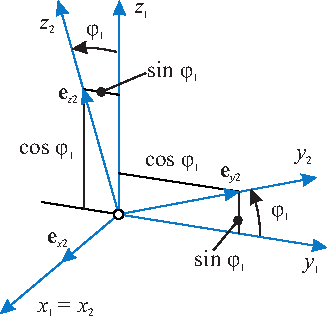
\includegraphics[height=6cm]{figures/elementaryRotationX}
%\caption{Elementary rotation around axis $\xv_1$.}
%\label{fig:theory:rotations:elementaryX}
%\end{center}
%\end{figure}
%
In a second example, a rotation with angle $\varphi_2$ around $\ev_{y2}$ is performed to transform from basis $(\ev_{x2},\,\ev_{y2},\,\ev_{z2})$ into $(\ev_{x3},\,\ev_{y3},\,\ev_{z3})$, see \fig{fig:theory:rotations:elementaryY}.
The rotation matrix for this case reads:
\be
  \LU{23}{\Rot} = \left[ \LUR{2}{\ev}{x3} \;\; \LUR{2}{\ev}{y3} \;\; \LUR{2}{\ev}{z3} \right] = 
  \mr{c \varphi_2}{0}{s \varphi_2}{0}{1}{0}{-s \varphi_2}{0}{c \varphi_2}\eqDot
\ee
%
\LatexRSTfigure{figures/elementaryRotationY}{fig:theory:rotations:elementaryY}{6cm}{320}{Elementary rotation around axis $\mathbf{ y}_2$.}
%\begin{figure}[htbp]
%\begin{center}
%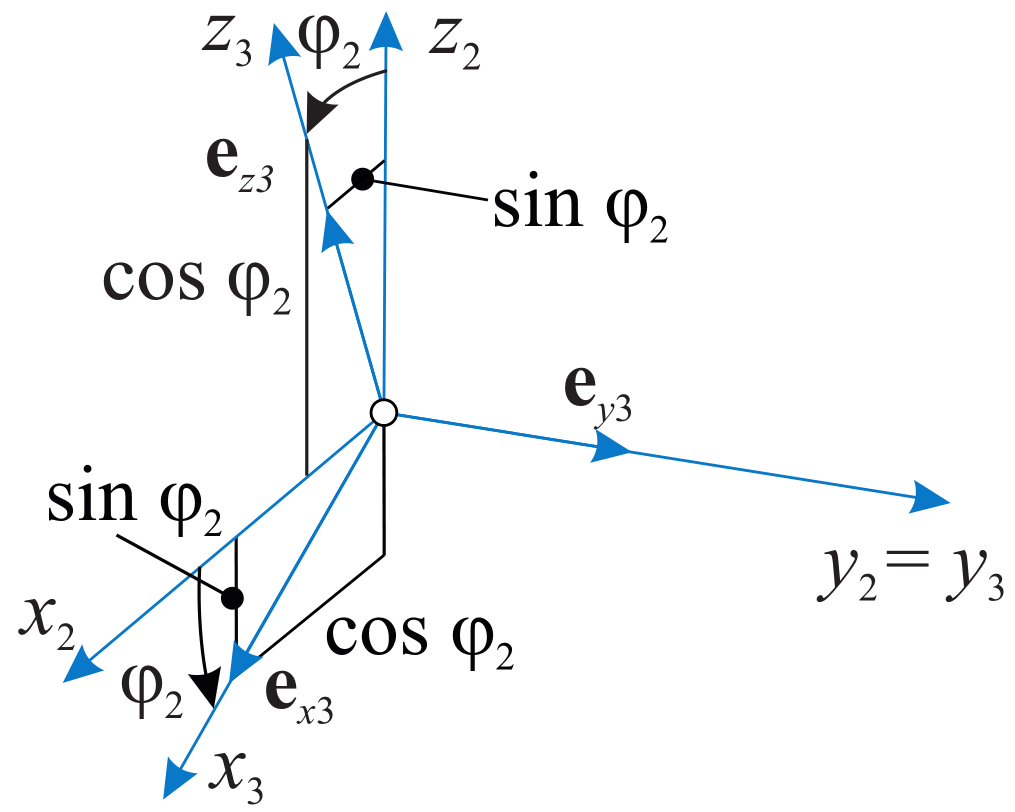
\includegraphics[height=4.5cm]{figures/elementaryRotationY}
%\caption{Elementary rotation around axis $\yv_2$.}
%\label{fig:theory:rotations:elementaryY}
%\end{center}
%\end{figure}
%
Finally, a rotation around $\ev_{z3}$ with angle $\varphi_3$ would give similarly,
\be
  \LU{34}{\Rot} = \left[ \LUR{3}{\ev}{x4} \;\; \LUR{3}{\ev}{y4} \;\; \LUR{3}{\ev}{z4} \right] = 
  \mr{c \varphi_3}{-s \varphi_3}{0} {s \varphi_3}{c \varphi_3}{0} {0}{0}{1} \eqDot
\ee



%+++++++++++++++++++++++++++++++++++++++++++++++++++++++++++++++++++++++++++++++
\mysubsubsubsection{Linearized rotations}
%add link to Rodrigues formula, immediately gives linearized case
%add link to linearized elementary rotations, off-diagonal components added
%add link to Im + skew(phi1, phi2, phi3), resulting from phi = delta t*omega; r2= r1+ delta t*(omega x r1) = (I + tilde phi) r1

In this case we can interpret the small rotations as a constant angular velocity over small time $\Delta t$, $\tvarphi = \Delta t \cdot \tomega$, which results in
\be
  \rv_1^\prime= \rv_1 + \Delta t \cdot (\tomega \times \rv_1) = (\Im + \tilde \tvarphi) \rv_1
\ee
Leading to the linearized rotation matrix
\be
  \Rot_\mathrm{lin} = \Im - \tilde \tvarphi
\ee

Alternatively, using linearized rotations $\tvarphi = [\varphi_1,\;\varphi_2,\;\varphi_3]\tp$, with $|\tvarphi| \ll 1$, we can approximate $\sin \varphi_1$ as:
\be
  \sin \varphi_1 = \varphi_1 - \frac{\varphi_1^3}{3!} + \frac{\varphi_1^5}{5!} - ... \approx \varphi_1
\ee
Similarly, we can approximate $\cos \varphi_1 \approx 1$. This immediately gives a linearization for elementary rotations -- where we observe that contributions for each axis can be added.

The axis-angle representation (see later) leads to the same result by linearization of the Rodrigues formula,
\be
  \Rot(\uv, \varphi) \approx \Im + \tilde \uv \varphi, \quad \Rot\tp \approx \Im - \tilde \uv \varphi
\ee
in which $\varphi$ represents the infinitesimal angle and $\uv$ is the rotation axis.

\mybold{Note}: whenever you would like to work with linearized rotations, or if you do not know the sequence of small rotations, still do not use the linearized formula as it gives immediately rotation matrices without strict orthogonality and determinant of 1. In order to avoid computational problems, use for example \texttt{RotationVector2RotationMatrix(phi)} to compute a consistent rotation matrix based on the matrix exponential.


%+++++++++++++++++++++++++++++++++++++++++++++++++++++++++++++++++++++++++++++++
\mysubsubsubsection{Active and passive rotations}
%
It is important to distinguish two fundamentally different concepts of rotations.
There is the \mybold{active rotation}, which can be represented by a coordinate-free relation,
\be \label{eq:theory:rotations:active}
  \vv^\prime = \Rot \vv
\ee
in which a vector $\vv$ is actively rotated into a new configuration $\vv^\prime$ using a rotation tensor $\Rot$.
\eq{eq:theory:rotations:active} can be represented in any coordinate system, but keeping it fixed.

Furthermore, we denote a \mybold{passive rotation} as a coordinate transformation, as used many times before,
\be
  \LU{1}{\vv} = \LU{12}{\Rot} \LU{2}{\vv}
\ee
in which the vector $\vv$ is not changed at all, but only its coordinates are represented in two different coordinate systems.

While passive rotations (and homogeneous transformations) are used, e.g., to compute current positions of body-attached points through several relative coordinate systems, active rotations can represent the rotations from one time step to the next one.

%+++++++++++++++++++++++++++++++++++++++++++++++++++++++++++++++++++++++++++++++
\mysubsubsubsection{Successive rotations}
%
The successive application of rotation matrices is non-commutative. An exception is the planar case, i.e., all rotations occur around the same axis.
Specifically, we see that for successive rotations, the following must be considered:
\be
  \Am_2 \Am_1 \vv \neq \Am_1 \Am_2 \vv \eqDot
\ee
As an example, we consider in Figure \ref{fig:theory:rotations:successive} the different order of rotations of a block.
%
\LatexRSTfigure{figures/RotationsSequences}{fig:theory:rotations:successive}{12cm}{500}{Successive rotations are not commutative.}
%\begin{figure}[tbph]
%\begin{center}
%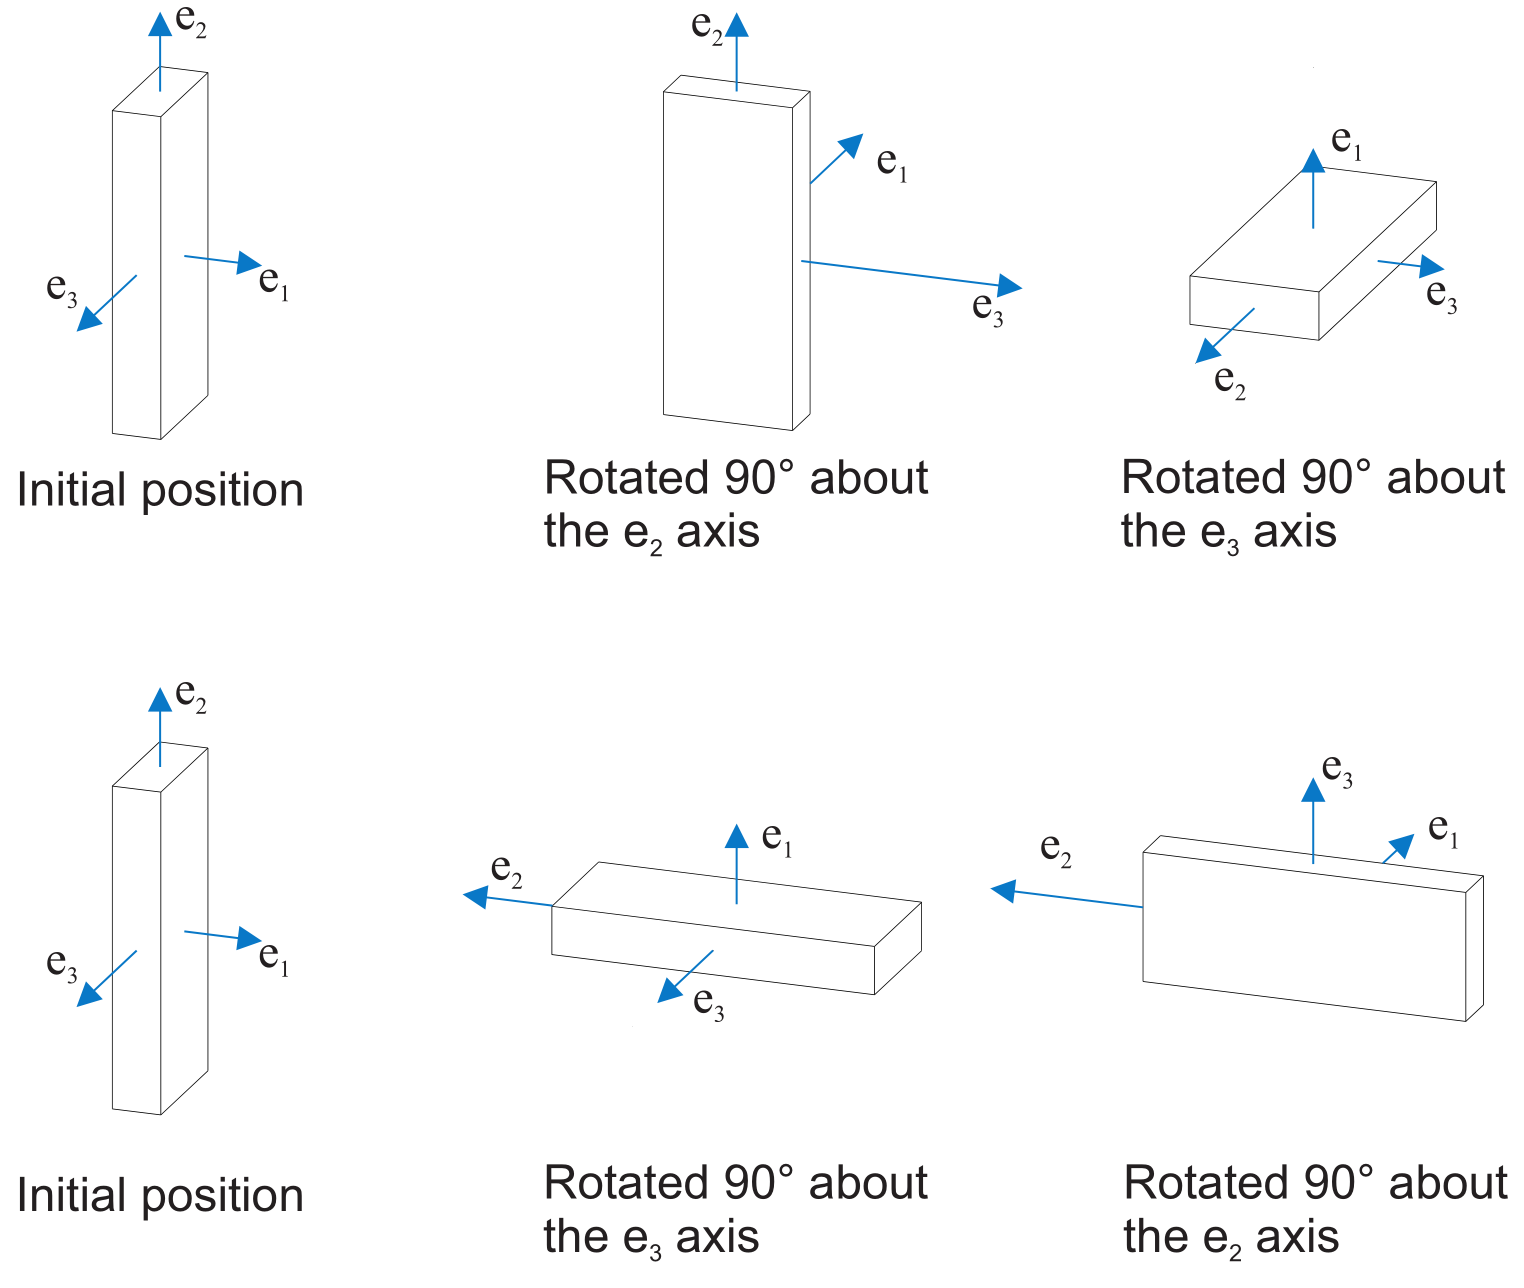
\includegraphics[width=12cm]{figures/RotationsSequences}
%\caption{Successive rotations.}
%\label{fig:theory:rotations:successive}
%\end{center}
%\end{figure}
%

In \fig{fig:theory:rotations:successive}a, the block shown is first rotated 90\textdegree about the $\mathbf{e}_2$ axis and then 90\textdegree about the $\mathbf{e}_3$ axis. In Figure \ref{fig:theory:rotations:successive}b, the same rotations are applied in reverse order, i.e., the block is first rotated 90\textdegree about the $\mathbf{e}_3$ axis and then 90\textdegree about the $\mathbf{e}_2$ axis. It is immediately apparent that the resulting orientation of the block is different in both cases.
%
%

Finally, it should be noted that there are two different types of successive rotations.
In the first variant, also known as the \mybold{single-frame method}, the same reference frame is chosen for each rotation. This variant is best understood in the active rotation of vectors, where these rotations always take place, for example, in the global reference system.

In the second variant, also known as the \mybold{multi-frame method}, a new reference frame created by the preceding rotation is used for each rotation. This variant can be illustrated by applications in robotics (e.g., articulated arm robots), where (passive) rotations of the reference systems of the robot's respective arms occur, with each rotation taking place in the reference system of the preceding arm.


%+++++++++++++++++++++++++++++++++++++++++++++++++++++++++++++++++++++++++++++++
%+++++++++++++++++++++++++++++++++++++++++++++++++++++++++++++++++++++++++++++++
\mysubsubsection{Rotation tensor: axis-angle representation}
%properties of rotation tensor
%update node (refer to this section!)
%Rodriguez formula (MKD-Sim2023 fig+formulas) (Drehzeiger)
In the following, we will elaborate the rotation tensor, inherently linked to the axis-angle representation.
Note that the rotation axis times the angle is denoted as rotation vector throughout.

Considering Euler's theorem on rotations, we assume a transformation
\be
  \rv_0 \ra \rv(t)
\ee
which purely follows from a rotation. This transformation thus can be represented by a rotation axis $\uv$ and an angle $\varphi(t)$,
\be
  (\uv(t), \, \varphi(t))
\ee
both of them given in a coordinate-free manner.
We may therefore conclude
\be %\label{eq:theory:rotations:rotationTensor}
  \rv(t)=\Rot(t) \, \rv_0 \qquad \text{with} \qquad \Rot(t)=\Rot(\uv(t),\varphi(t))
\ee
%
\LatexRSTfigure{figures/RotationAxisAngle}{fig:theory:rotations:angleAxis}{6cm}{260}{Rotation of a vector $\mathbf{ r}_0$ by means of the angle-axis tuple $(\mathbf{ u}(t), \, \varphi(t))$.}
%\begin{figure}[tbph]
%\begin{center}
%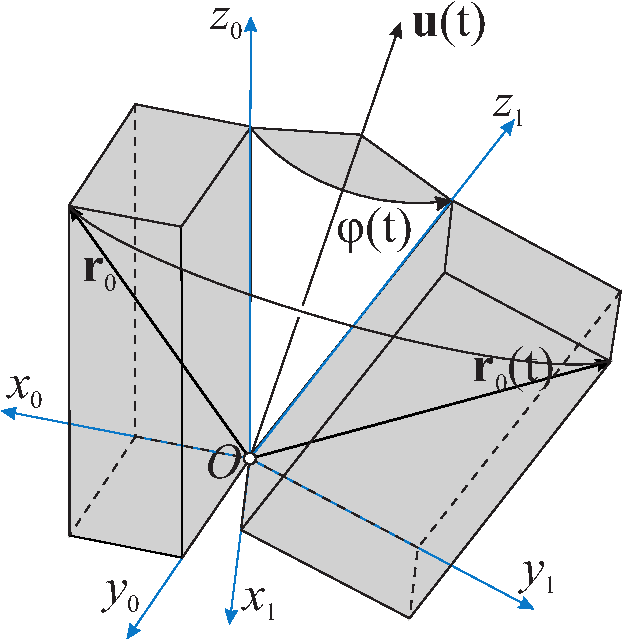
\includegraphics[width=12cm]{figures/RotationAxisAngle}
%\caption{Rotation of a vector $\rv_0$ by means of the angle-axis tuple $(\uv(t), \, \varphi(t))$.}
%\label{fig:theory:rotations:angleAxis}
%\end{center}
%\end{figure}
%

Using \fig{fig:theory:rotations:angleAxis}, we may now consider relations of the two frames $(\ev_{x0},\,\ev_{y0},\,\ev_{z0})$ and $(\ev_{x1},\,\ev_{y1},\,\ev_{z1})$, solely defined by the angle-axis $(\uv(t), \, \varphi(t))$ relation.
%
\LatexRSTfigure{figures/RotationAxisAngleDerivation}{fig:theory:rotations:axisAngleDerivation}{7cm}{320}{Relations for derivation of rotation tensor and Rodrigues' formula.}
%\begin{figure}[tbph]
%\begin{center}
%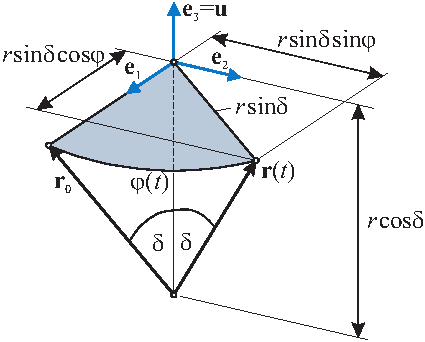
\includegraphics[width=12cm]{figures/RotationAxisAngleDerivation}
%\caption{Relations for derivation of rotation tensor and Rodrigues' formula.}
%\label{fig:theory:rotations:axisAngleDerivation}
%\end{center}
%\end{figure}
%

According to \fig{fig:theory:rotations:axisAngleDerivation}, we may split the vector $\rv$, which has the length $r = \vert \rv \vert$, into
\be 
  \rv= c_1 \ev_1 + c_2 \ev_2 + c_3 \ev_3 
\ee
with the unit vectors given as
\be
  \ev_1  =  \frac{\rv_0 - \uv(\uv^{\mathrm{T}} \rv_0)}{r \sin \delta},  \quad
  \ev_2  =  \frac{\tilde{\uv} \rv_0}{r \sin \delta}, \quad \mathrm{and} \quad 
  \ev_3  =   \uv \eqDot
\ee
The coefficients can be calculated as follows,
\be
  c_1 = r \sin \delta \cos \varphi, \quad
  c_2 = r \sin \delta \sin \varphi, \quad \mathrm{and} \quad
  c_3 = r \cos \delta
\ee
Putting everything together gives
\be 
  \rv = \cos \varphi \, \rv_0 + \sin \varphi \, \tilde{\uv} \, \rv_0 + (1 - \cos \varphi) \, \uv \, (\uv\tp \, \rv_0)
\ee
From the relation $\rv = \Rot(\uv ,\varphi) \rv_0$, we can reinterpret the \mybold{rotation tensor} $\Rot$
\be
  \Rot(\uv ,\varphi) = \cos \varphi \, \Im + \sin \varphi \, \tilde{\uv} + (1-\cos \varphi) \, \uv \, \uv\tp
\ee
%
With the additional relations
\be 
  \uv \, \uv\tp=\tilde\uv \, \tilde\uv +(\uv\tp \uv) \Im \quad \mathrm{and} \quad \uv\tp \uv = 1
\ee
we finally obtain
\be 
  \Rot(\uv ,\varphi) =  \Im + \sin \varphi \, \tilde{\uv} + (1-\cos \varphi) \,  \tilde{\uv} \, \tilde{\uv}
\ee
which is also known as the \mybold{Rodrigues formula} for rotations. 
While this formula is coordinate-free, it may be represented in any coordinate system, such as
\be 
  \LU{0}{\rv}(t)=\LU{0}{\Rot}(t) \, \LUR{0}{\rv}{0} \qquad \text{with} \qquad \LU{0}{\Rot}(t)=\Rot(\LU{0}{\uv}(t),\varphi(t))
\ee    

%+++++++++++++++++++++++++++++++++++++++++++++++++++++++++++++++++++++++++++++++
\mysubsubsubsection{Rotation vector}
%
Using the rotation vector $\vv_\mathrm{rot} = \varphi\cdot \uv$ and $\varphi = |\vv_\mathrm{rot}|$, another representation of the rotation tensor follows as
\be 
  \Rot(\uv ,\varphi) =  \Im + \frac{\sin \varphi}{\varphi} \tilde\vv_\mathrm{rot} + \frac{(1-\cos \varphi)}{\varphi^2} \,  \tilde\vv_\mathrm{rot} \, \tilde\vv_\mathrm{rot}
\ee
Note, that we inherently assume that $\varphi \in [0,\pi]$.
%
\noindent In \codeName, there are the following \mybold{functions and items related to the rotation vector} and the axis-angle representation:
\bi
  \item \texttt{NodeRigidBodyRotVecLG}: A 3D rigid body node based on rotation vector and Lie group methods; can be used for explicit integration methods, not leading to singularities when integrating with Lie-group methods
  \item \texttt{RotationVector2RotationMatrix}: computes the rotation matrix from a given rotation vector $\vv_\mathrm{rot}$
  \item \texttt{RotationMatrix2RotationVector}: computes the rotation vector $\vv_\mathrm{rot}$ from a given rotation matrix, based on a reconstruction of Euler parameters
  \item \texttt{ComputeRotationAxisFromRotationVector}: computes the rotation axis $\uv$ from the rotation vector by using $\varphi = |\vv_\mathrm{rot}|$
\ei
%
Note the following \mybold{properties of the rotation tensor}:
\bi
  \item The axis-angle representations $(\uv, \varphi)$ and $(-\uv, -\varphi)$ represent the same tensor $\Rot(\uv,\varphi)=\Rot(-\uv,-\varphi)$
  \item The rotation tensor $\Rot$ is orthogonal, i.e., $\Rot\tp \, \Rot = \Em$. 
  \item The inverse rotation tensor $\Rot^{-1} = \Rot\tp$ is represented by the identical axis-angle tuples $(\uv, -\varphi)$ and $(-\uv, \varphi)$, leading to $\rv_0=\Rot(\uv, -\varphi) \rv$.
  \item We furthermore not the identities: $\Rot(\uv, -\varphi) \equiv \Rot(-\uv, \varphi) \equiv \Rot\tp (\uv, \varphi)$
  \item The rotation axis is invariant to the rotation: $\Rot(\uv, \varphi) \uv = \uv$
  %
\ei


%+++++++++++++++++++++++++++++++++++++++++++++++++++++++++++++++++++++++++++++++
%+++++++++++++++++++++++++++++++++++++++++++++++++++++++++++++++++++++++++++++++
\mysubsubsection{Euler angles: Tait-Bryan angles}
%general explanation as Rx*Ry*Rz
%refer to node
%update node (refer to this section!)
%include relations with angular velocity
%see robotics / EMKL script page 33
In the following section, we discuss rotation matrices built by Tait-Bryan angles, which are consecutive $xyz$-rotations.
Note that there are many other representations of Euler angles, however, they are not implemented or used in \codeName.
The output variable \texttt{Rotation} gives Tait-Bryan angles, which is why it is important to define their properties.

%
\LatexRSTfigure{figures/theoryRotationsTaitBryanAngles}{fig:theory:rotations:TaitBryanAngles}{8cm}{240}{Definition of Tait-Bryan angles.}
%\begin{figure}[tbph]
%\begin{center}
%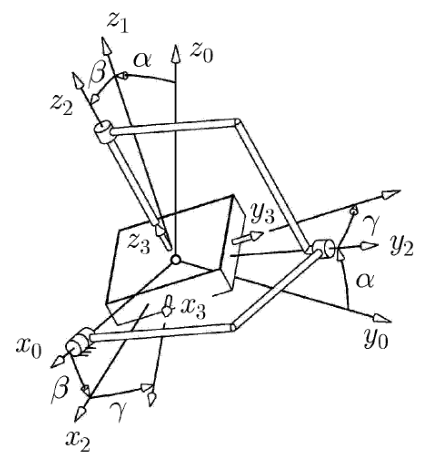
\includegraphics[width=12cm]{figures/theoryRotationsTaitBryanAngles}
%\caption{Definition of Tait-Bryan angles.}
%\label{fig:theory:rotations:TaitBryanAngles}
%\end{center}
%\end{figure}
%

\noindent The transformation given by Tait-Bryan angles $(\alpha,\beta,\gamma)$ follows from three successive rotations,
\be
  \LU{0}{\rv} = \LU{01}{\Rot}(\alpha) \, \LU{12}{\Rot}(\beta) \, \LU{23}{\Rot}(\gamma) \, \LU{3}{\rv} \quad
  \mathrm{and} \quad \LU{0}{\rv} = \LU{03}{\Rot}(\alpha,\beta,\gamma) \, \LU{3}{\rv}
\ee
The \mybold{Tait-Bryan rotation matrix} is thus defined as
\be
  \LU{03}{\Rot}(\alpha,\beta,\gamma) = \mr{\co\beta \,\co\gamma}{-\co\beta\,\si\gamma}{\si\beta} {\co \alpha \,\si \gamma + \si \alpha \,\si \beta \,\co \gamma}{\co \alpha \,\co\gamma-\si\alpha\,\si\beta\,\si\gamma}{-\si\alpha\,\co\beta} {\si\alpha\,\si\gamma-\co\alpha\,\si\beta\,\co\gamma}{\si\alpha\,\co\gamma+\co\alpha\,\si\beta\,\si\gamma}{\co\alpha\,\co\beta}
\ee
While not fully obvious from the latter equations, we note that there is a singularity at $|\beta| = \frac{\pi}{2}$, which causes any computations to stall whenever getting close enough to this value.

\noindent It is also possible to reconstruct Tait-Bryan angles from a given rotation matrix.
Assume, we have the rotation matrix $\LU{03}{\Rot}=(A_{ij})$.
There are two solutions for $\beta$ which follow from
\be
  \cos \beta = \pm \sqrt{1-A_{13}^2}, \quad \mathrm{and} \quad \sin \beta = A_{13}
\ee
For beta fulfilling $|\beta| \ne \frac{\pi}{2}$, we can uniquely compute $\gamma$ and $\alpha$,
\be
  \cos \gamma = \frac{A_{11}}{\cos \beta}, \quad \sin \gamma = - \frac{A_{12}}{\cos \beta}, \quad
  \cos \alpha = \frac{A_{33}}{\cos \beta}, \quad \mathrm{and} \quad \sin \alpha = - \frac{A_{23}}{\cos \beta} \eqDot
\ee
Note that improvements are possible using the $\mathrm{atan2}()$ function.
We can finally resolve non-uniqueness by restricting $\beta$ within the range $-\frac{\pi}{2} < \beta < \frac{\pi}{2}$.

\mysubsubsubsection{Tait-Bryan angles: angular velocity vector}
%
Angular velocities are essential for the formulation of equations of motion of rigid bodies, for constraints and for evaluation.
Therefore, basic relations are shown for Tait-Bryan angles, in particular the velocity transformation matrix $\Gm_{TB}$.

The angular velocity vector $\omega$ can either be computed from the basic relation $\dot \Rot = \tilde \omega \Rot$, which however involves many trigonometric terms, or from partial angular velocities, being part of the co-rotated rotation axes.
With the latter approach, we see that
\be
  \tomega_{30}=\dot{\alpha} \ev_{x0}+\dot{\beta} \ev_{y1}+\dot{\gamma} \ev_{z2} \quad \text{or} \quad 
  \tomega_{30}=\underbrace{[\ev_{x0} \quad \ev_{y1} \quad \ev_{z2}]}_{\Gm_{TB}} \vr{\dot{\alpha}}{\dot{\beta}}{\dot{\gamma}}
\ee
We can now evaluate this equation in frame $\mathcal{F}_0$ with $\tbeta=[\alpha\;\beta\;\gamma]\tp$, written as
\be 
  \LUR{0}{\tomega}{30}=\underbrace{[\LUR{0}{\ev}{x0} \quad \LUR{0}{\ev}{y1} \quad \LUR{0}{\ev}{z2}]}_{\LUR{0}{\Gm}{TB}} \vr{\dot{\alpha}}{\dot{\beta}}{\dot{\gamma}} = 
  \LUR{0}{\Gm}{TB}(\tbeta) \dot{\tbeta} \eqDot
\ee
Evaluating the consecutive rotations, we find the respective unit vectors as
\be
  \LUR{0}{\ev}{x0} = \vr{1}{0}{0}, \quad
  \LUR{0}{\ev}{y1} = \vr{0}{\text{c} \alpha}{\text{s} \alpha}, \quad \mathrm{and} \quad
  \LUR{0}{\ev}{z2} = \vr{\text{s} \beta}{-\text{s} \alpha \text{c} \beta}{\text{c} \alpha \text{c} \beta} \eqDot
\ee
which results in the relations for the (global) angular velocity vector
\be \label{eq:theory:rotations:TaitBryanG}
  \vr{\LUR{0}{\omega}{30x}}{\LUR{0}{\omega}{30y}}{\LUR{0}{\omega}{30z}} = 
  \mr{1}{0} {\text{s} \beta}
  {0}{\text{c} \alpha} {-\text{s} \alpha \text{c} \beta}
  {0}{\text{s} \alpha} {\text{c} \alpha \text{c} \beta}  
  \vr{\dot{\alpha}}{\dot{\beta}}{\dot{\gamma}} 
\ee
The matrix $\LUR{0}{\Gm}{TB}$ is used to compute partial derivatives of the angular velocity vector w.r.t.\ rotations.
However, it is also used to project torques and angular velocities into a space given by $\Gm_{TB}^\mathrm{T}$ (which is indeed not equivalent to $\Gm_{TB}^{-1}$, but gives a symmetric mass matrix -- see the equations of motion for the rigid body).

The inverse relation between $\dot \tbeta$ and $\LUR{0}{\tomega}{30}$ gives
\be \label{eq:theory:rotations:TaitBryanGinv}
  \vr{\dot{\alpha}}{\dot{\beta}}{\dot{\gamma}} = \frac{1}{\text{c} \beta} \mr{\text{c} \beta}{\text{s} \alpha \, \text{s} \beta}{-\text{c} \alpha \, \text{s} \beta}{0}{\text{c} \alpha \, \text{c} \beta}{\text{s} \alpha \text{c} \beta}{0}{-\text{s} \alpha}{\text{c} \alpha}  \vr{\LUR{0}{\omega}{30x}}{\LUR{0}{\omega}{30y}}{\LUR{0}{\omega}{30z}}
\ee
or in compact form
\be
  \dot{\tbeta} = \LURU{0}{\Gm}{TB}{-1}(\tbeta)  \LUR{0}{\tomega}{30}
\ee
We again see that for the case $\vert \beta \vert = \pi/2$ the matrix$\LUR{0}{\Gm}{TB}$ becomes singular, and \eq{eq:theory:rotations:TaitBryanGinv} cannot be resolved for $\dot{\tbeta}$!

\noindent Finally, we also provide the relations of $\tomega_{30}$ in body-fixed (local) coordinates $\mathcal{F}_3$,
which are frequently used in the implementation,
\be
  \vr{\LUR{3}{\omega}{30x}}{\LUR{3}{\omega}{30y}}{\LUR{3}{\omega}{30z}} = \mr{\text{c} \beta \, \text{c} \gamma}{\text{s} \gamma}{0}{-\text{c} \beta \, \text{s} \gamma}{\text{c} \gamma}{0}{\text{s} \beta}{0}{1} \vr{\dot{\alpha}}{\dot{\beta}}{\dot{\gamma}} \eqComma
\ee
which reads in compact form ($\LUR{3}{\Gm}{TB} = \LUR{b}{\Gm}{TB}$),
\be
  \LUR{3}{\tomega}{30} =  \LUR{3}{\Gm}{TB}(\tbeta) \dot{\tbeta}
\ee

\noindent In \codeName, there are the following \mybold{functions and items related to Tait-Bryan angles}:
\bi
  \item \texttt{NodeRigidBodyRxyz}: A 3D rigid body node based on Tait-Bryan angles
  \item \texttt{RotXYZ2RotationMatrix}: computes the rotation matrix from given Tait-Bryan angles
  \item \texttt{RotationMatrix2RotXYZ}: computes Tait-Bryan angles from a given rotation matrix
  \item \texttt{RotXYZ2G}: computes the matrix $\LU{0}{\Gm}$ relating time derivatives of Tait-Bryan angles to the (global) angular velocity vector
  \item \texttt{RotXYZ2Glocal}: computes the matrix $\LU{b}{\Gm}$ relating time derivatives of Tait-Bryan angles to the (local, body-fixed) angular velocity vector
\ei



%+++++++++++++++++++++++++++++++++++++++++++++++++++++++++++++++++++++++++++++++
%+++++++++++++++++++++++++++++++++++++++++++++++++++++++++++++++++++++++++++++++
\mysubsubsection{Euler parameters and unit quaternions}
%refer to node
%update node (refer to this section!)

As one of the most important forms of rotational parameters for multibody systems, the 4 Euler parameters are introduced.
They can be mathematically represented as unit quaternions and provide particularly simple expressions and equations of motion, albeit at the expense of an additional constraint.

The Euler parameters are defined as
\be \label{eq:theory:rotations:eulerParametersDef}
  \underline{\pv}=\vp{p_{\mathrm{s}}}{\pv}=\vp{\cos \frac \varphi 2}{\uv \, \sin \frac\varphi 2} \quad \text{bzw.} \quad \underline{\pv}=\vfour{p_{\mathrm{s}}}{p_x}{p_y}{p_z}=\vfour{\cos \frac\varphi 2}{u_x \, \sin \frac\varphi 2}{u_y \, \sin \frac\varphi 2}{u_z \, \sin \frac\varphi 2}
\ee
Here, $p_s=\cos \frac\varphi 2$ is the scalar part and $\pv = \uv \, \sin \frac\varphi 2$ is the vector part of the Euler parameters $\underline{\pv}$.
The four Euler parameters $\underline{\pv}$ are subject to the normalization condition
\be 
  \phi(\underline{\pv}) \equiv p_s^2+p_x^2+p_y^2+p_z^2-1=0 \quad \mathrm{or} \quad  p_s^2 +\pv\tp \, \pv -1 = 0 \eqDot
\ee
First, the following trigonometric transformations are introduced,
\be
  \cos \varphi = 2 \cos^2\frac{\varphi}{2} -1, \quad \sin \varphi = 2 \sin \frac \varphi 2 \cos \frac \varphi 2, \quad 1-\cos \varphi = 2 \sin^2 \frac{\varphi}{2} \eqDot
\ee
When these are substituted into the rotation tensor using \eq{eq:theory:rotations:eulerParametersDef}, it follows
\be 
  \Rot(\underline{\pv})=(2 p_{\mathrm{s}}^2-1) \, \Em + 2 p_{\mathrm{s}} \, \tilde{\pv} + 2 \, \pv \, \pv\tp \eqDot
\ee

Euler parameters can initially be expressed in the global reference frame $\mathcal{F}_0$,
\be
  \LU{0}{\underline{\pv}}=\vp{p_{\mathrm{s}}}{\LU{0}{\pv}}=\vp{\cos \frac\varphi 2}{\LU{0}{\uv} \, \sin \frac{\varphi} {2}} \eqDot
\ee
Thus, the coordinate representation of the rotation tensor is given by
\be \label{eq:theory:rotations:eulerParametersRot}
  \Rot(\LU{0}{\underline{\pv}}) = 2 \LU{0}{\mr{\ps^2+p_x^2-\frac 1 2}{p_x p_y-\ps p_z}{p_x p_z+\ps p_y} 
                                {p_x p_y+\ps p_z}{\ps^2+p_y^2-\frac 1 2}{p_y p_z-\ps p_x} 
                                {p_x p_z-\ps p_y}{p_y p_z+\ps p_x}{\ps^2+p_z^2-\frac{1}{2} }} = \LU{01}{\Rot}
\ee
Note that the axis of rotation is invariant to the rotation, $\LU{0}{\uv} = \LU{1}{\uv}$, thus $\LU{0}{\underline{\pv}} = \LU{1}{\underline{\pv}}$
Due to the ambiguity $\Rot(\underline{\pv}) = \Rot(-\underline{\pv})$, the scalar part of the Euler parameters is usually normalized, i.e., $p_s \ge 0$.

\noindent The careful reader may observe that matrix $\Rot$ in \eq{eq:theory:rotations:eulerParametersRot} is not identical to the implementation in \codeName.
This is true, because there is always an alternative formulation for the diagonal terms by adding the normalization condition times a factor.

%+++++++++++++++++++++++++++++++++++++++++++++++++++++++++++++++++++++++++++++++
\mysubsubsubsection{Quaternion operations}
%
Calculations with Euler parameters are efficiently performed through the rules of quaternion algebra.
Active perspective as vector rotation: The rotation of vector $\rv_0$ into $\rv(t)$,
\be \label{eq:theory:rotations:quaternionRotation}
  \LU{0}{\rv}(t)=\LU{0}{\Rot}(t) \, \LUR{0}{\rv}{0} \quad \text{mit} \quad \LU{0}{\Rot}(t)= \Rot(\LU{0}{\uv}(t), \varphi (t))
\ee
is formulated using the quaternion $\LU{0}{\underline{\pv}}=\underline{\pv}(\LU{0}{\uv}, \varphi)$ and its conjugate $\myoverline{\underline{\pv}}$ with the help of the double quaternion product (operator $\circ$),
\be 
  \LU{0}{\underline{\rv}}(t) = \LU{0}{\underline{\pv}}(t) \, \circ \, \LUR{0}{\underline{\rv}}{0} \, \circ \, \LU{0}{\underline{\myoverline{\pv}}}(t) \eqComma
\ee
or in short form,
\be
\vp{0}{\LU{0}{\rv}(t)}=\vp{p_{\mathrm{s}}(t)}{\LU{0}{\pv}(t)} \, \circ \, \vp{0}{\LUR{0}{\rv}{0}} \, \circ \, \vp{p_{\mathrm{s}}(t)}{-\LU{0}{\pv}(t)} \eqDot
\ee
With the multiplication rule for quaternions, the scalar part yields $0=0$ and the vector part the vector rotation \eqref{eq:theory:rotations:quaternionRotation}. 
For multiple rotations, we have
\be
  \LUR{0}{\underline{\rv}}{2}=\LUR{0}{\underline{\pv}}{2} \circ \LUR{0}{\underline{\pv}}{1} \circ \LUR{0}{\underline{\rv}}{0} \circ  \LUR{0}{\myoverline{\underline{\pv}}}{1} \circ \LUR{0}{\myoverline{\underline{\pv}}}{2} \eqDot
\ee
Given two quaternions
\be
  \underline{\av} = a_\mathrm{s} + \mathrm{i}\, a_x + \mathrm{j}\, a_y + \mathrm{k}\, a_z, \quad \mathrm{and} \quad \underline{\bv} = b_\mathrm{s} + \mathrm{i}\, b_x + \mathrm{j}\, b_y + \mathrm{k}\, b_z \eqComma
\ee
we provide two important \mybold{rules of quaternion algebra}, which is the sum,
\be
  \underline{\cv} = \underline{\av} + \underline{\bv} \quad \ra \quad 
  \vp{c_\mathrm{s}}{\cv} = \vp{a_\mathrm{s}}{\av} + \vp{b_\mathrm{s}}{\bv} = \vp{a_\mathrm{s} + b_\mathrm{s}}{\av + \bv} \eqComma
\ee
and the multiplication
\be
  \underline{\cv} = \underline{\av} \circ \underline{\bv} \neq \underline{\bv} \circ \underline{\av} \quad \ra \quad
  \vp{c_\mathrm{s}}{\cv} = \vp{a_\mathrm{s}}{\av} \circ \vp{b_\mathrm{s}}{\bv} = 
   \vp{a_\mathrm{s} b_\mathrm{s} - \av^\mathrm{T} \bv}{a_\mathrm{s}\bv + b_\mathrm{s}\av + \tilde \av \bv} \eqDot
\ee


%+++++++++++++++++++++++++++++++++++++++++++++++++++++++++++++++++++++++++++++++
\mysubsubsubsection{Angular velocity vector}
%
To derive the angular velocity from Euler parameters, there are both the possibilities of deriving the rotation matrix with respect to time and directly deriving the angular velocity from Euler parameters.

\noindent For an infinitesimal rotation $\dd \psi$, the quaternion follows
\be
  \underline{\pv}(\ev, \dd \psi) = \vp{\cos \frac{\dd \psi}{2}}{\ev \sin \frac{\dd\psi}{2}} \approx 
    \vp{1}{\ev \frac{\dd\psi}{2}}
\ee
from which we conclude that from $\underline{\pv}(\ev, \dd \psi) \, \circ \, \underline{\pv}(t) = \underline{\pv}(t) + \dd\underline{\pv}$ and thus $\dd\underline{\pv} = \vp{0}{\ev \frac{\dd\psi}{2}}$.
Dividing by $\dd t$ and with the angular velocity $\tomega_{10} = \ev \, \dot \psi$, it follows
\be
  \vp{\dot \ps}{\LLdot{0}{\pv}{}} = \frac{1}{2} \vp{0}{\tomega_{10} }  \circ \vp{\ps}{\pv}
\ee
or in short form
\be
  \LU{0}{\underline{\dot \pv}} = \frac{1}{2} \underline{\tomega}_{10}  \circ \underline{\pv}
\ee
With the quaternion product in matrix notation, it follows
\be
  \vp{\dot \ps}{\LU{0}{\dot\pv}{}} = \frac{1}{2} \mp{\ps}{-\pv^\mathrm{T}}{\pv}{\ps \Em - \tilde \pv} \vp{0}{\tomega_{10} }
\ee
or with the matrix $\underline{\Pm}$ it can be written as
\be
  \LU{0}{\underline{\dot \pv}}{} = \frac{1}{2} {\underline{\Pm}}(\pv) \underline{\tomega}_{10}    
\ee
This form can be represented in global coordinates due to ${\underline{\Pm}}^{-1} = {\underline{\Pm}}\tp$ as
\be
  \vp{0}{\LU{0}{\tomega}_{10} } = 2 \mp{\ps}{\LU{0}{\pv}^\mathrm{T}}{-\LU{0}{\pv}}{\ps \Em + \LU{0}{\tilde \pv}} \, \vp{\dot \ps}{\LLdot{0}{\pv}{}}
\ee
Thus, the velocity transformation follows to
\be
  \LUR{0}{\Gm}{EP} = \left[-2\LU{0}{\pv}, \; 2\ps \Em + 2\LU{0}{\tilde \pv}\right]
\ee
as a matrix with 3 rows and 4 columns. With $\LUR{0}{\Gm}{EP}$, the angular velocity vector can be conveniently calculated,
\be
  \LU{0}{\tomega}_{10} = \left[-2\LU{0}{\pv}, \; 2\ps \Em + 2\LU{0}{\tilde \pv}\right] \, \LU{0}{\underline{\dot \pv}}
\ee

\noindent In \codeName, there are the following \mybold{functions and items related to Euler parameters}:
\bi
  \item \texttt{NodeRigidBodyEP}: A 3D rigid body node based on Euler parameters
  \item \texttt{EulerParameters2RotationMatrix}: computes the rotation matrix from given Euler parameters
  \item \texttt{RotationMatrix2EulerParameters}: computes Euler parameters from a given rotation matrix
  \item \texttt{EulerParameters2G}: computes the matrix $\LUR{0}{\Gm}{EP}$ relating time derivatives of Euler parameters to the (global) angular velocity vector
  \item \texttt{EulerParameters2Glocal}: computes the matrix $\LUR{b}{\Gm}{EP}$ relating time derivatives of Euler parameters to the (local, body-fixed) angular velocity vector
\ei



%+++++++++++++++++++++++++++++++++++++++++++++++++++++++++++++++++++++++++++++++
%+++++++++++++++++++++++++++++++++++++++++++++++++++++++++++++++++++++++++++++++
\mysubsectionlabel{Integration Points}{sec:integrationPoints}
For several tasks, especially for finite elements and contact, different integration rules are used, which are summarized here.
The interval of all integration rules is $\in [-1,1]$, thus giving a total sum for integration weights of 2.
The points $\xi_{ip}$ and weights $w_{ip}$ for Gauss rules read:

The following table collects some typical \mybold{input parameters} for nodes, objects and markers: \vspace{-12pt}
\startGenericTable{| c | c | c | c | c |}
\rowTableFive{\mybold{type/order}}{ \mybold{point 0}}{ \mybold{point 1}}{ \mybold{point 2}}{ \mybold{point 3} }
\rowTableFive{Gauss 1}{ 0}{}{}{}
\rowTableFive{Gauss 3}{ $-\sqrt{1 / 3}$}{ $\sqrt{1 / 3}$}{}{}
\rowTableFive{Gauss 5}{ $-\sqrt{3 / 5}$}{ 0}{ $\sqrt{3 / 5}$}{}
\rowTableFive{Gauss 7}{ $-\sqrt{3 / 7 + \sqrt{120} / 35}$}{ $-\sqrt{3 / 7 - \sqrt{120} / 35}$}{ $\sqrt{3 / 7 - \sqrt{120} / 35}$}{ $\sqrt{3 / 7 + \sqrt{120} / 35}$ }
\rowTableFive{}{}{}{}{}
\rowTableFive{\mybold{type/order}}{ \mybold{weight 0}}{ \mybold{weight 1}}{ \mybold{weight 2}}{ \mybold{weight 3} }
\rowTableFive{Gauss 1}{ 2}{}{}{}
\rowTableFive{Gauss 3}{ 1}{ 1}{}{}
\rowTableFive{Gauss 5}{ $5 / 9$}{ $8 / 9$}{ $5 / 9$}{ }
\rowTableFive{Gauss 7}{ $1 / 2 - 5 / (3 \sqrt{120})$}{ $1 / 2 + 5 / (3*\sqrt{120})$}{ $1 / 2 + 5 / (3*\sqrt{120})$}{ $1 / 2 - 5 / (3*\sqrt{120})$ }
\finishTable

The points $\xi_{ip}$ and weights $w_{ip}$ for Lobatto rules read: \vspace{-12pt}
\startGenericTable{| c | c | c | c | c |}
\rowTableFive{\mybold{type/order}}{ \mybold{point 0}}{ \mybold{point 1}}{ \mybold{point 2}}{ \mybold{point 3}}
\rowTableFive{Lobatto 1}{ -1}{ 1}{}{}
\rowTableFive{Lobatto 3}{ -1}{ 0}{ 1}{}
\rowTableFive{Lobatto 5}{ -1}{ $-\sqrt{1/5}$}{ $\sqrt{1/5}$}{ 1}
\rowTableFive{}{}{}{}{}
\rowTableFive{\mybold{type/order}}{ \mybold{weight 0}}{ \mybold{weight 1}}{ \mybold{weight 2}}{ \mybold{weight 3} }
\rowTableFive{Lobatto 1}{ 1}{ 1}{}{}
\rowTableFive{Lobatto 3}{ $1/3$}{ $4/3$}{ $1/3$}{}
\rowTableFive{Lobatto 5}{ $1/6$}{ $5/6$}{ $5/6$}{ $1/6$}
\finishTable
Further integration rules can be found in the C++ code of \codeName, see file \texttt{BasicLinalg.h}.




%+++++++++++++++++++++++++++++++++++++++++++++++++++++++++++++++++++++++++++++++++++++++++++
\newpage
\mysubsectionlabel{Model order reduction and component mode synthesis}{sec:theory:CMS}
%terminology: eigenmode, eigenvector, eigenvalue, normal mode, static mode

This section describes the process how to create general flexible multibody system models using the floating frame of reference formulation with model order reduction (here also denoted as \hac{CMS}). The according object \texttt{ObjectFFRFreducedOrder} is described in \refSection{sec:item:ObjectFFRFreducedOrder}.

\mysubsubsection{Import of flexible bodies}
%
For flexible bodies in multibody systems, specifically for model order reduction, a standard input data (SID) has been defined in the past \cite{Schwertassek1999}.
A recent formulation for \ac{FFRF} \cite{ZwoelferGerstmayr2021} showed that significantly less information is required for the computation of the dynamics of displacement-based solid finite elements:
\bi
  \item nodal reference positions (given in \texttt{FEMinterface} member variable \texttt{nodes['Position']})
  \item stiffness matrix (given in \texttt{FEMinterface} member variable \texttt{stiffnessMatrix})
  \item mass matrix (given in \texttt{FEMinterface} member variable \texttt{massMatrix})
  \item (given in \texttt{FEMinterface} member variable \texttt{nodes['Position']})
\ei
In addition, the following data may be needed:
\bi
  \item element connectivity: needed for visualization, surface reconstruction and stress computation
  \item list of surface elements: if not computed internally in \codeName (stored in \texttt{FEMinterface} member variable \texttt{surface})
  \item information on how to obtain stresses from the set of (reduced) coordinates:  if not computed internally in \codeName (stored in \texttt{FEMinterface} member variable \texttt{postProcessingModes} for stresses at nodal positions)
\ei
This data can be generated by an appropriate interface to NGsolve:
\bi
  \item \texttt{FEMinterface.ImportMeshFromNGsolve(...)},
\ei
or imported from ABAQUS with \texttt{FEMinterface} functions
\bi
  \item \texttt{ReadMassMatrixFromAbaqus(...)}, 
  \item \texttt{ReadStiffnessMatrixFromAbaqus(...)}, 
  \item \texttt{ImportFromAbaqusInputFile(...)} )
\ei
and similar functionality exists for ANSYS.
Importing data may be time consuming, which is why all FEMinterface data, including computed modes, can be saved and loaded via
\texttt{SaveToFile} and \texttt{LoadFromFile}. 

It is assumed that there exists an underlying solid finite element mesh, given by e.g., tetrahedral or hexahedral finite elements. However, this mesh is not needed for computations. If the surface or any part of the flexible body shall be visualized, surface elements (triangles or quads) need to be provided with indices of the mesh nodes. The computation of surface elements is done by \texttt{FEMinterface} function \texttt{ VolumeToSurfaceElements}, making use of solid finite elements stored in \texttt{FEMinterface.elements}.

A major advantage of the \texttt{FEMinterface} data is that it is widely independent of underlying finite element technologies, specifically finite element order, reduced integration, etc., however, stress or strain can not be computed as well.
A conventional way is to store computed body deformations and perform post processing in the original finite element code, which gives highest quality of stress, strain, and other quantities.
A second way is, due to linearity of the small deformation assumptions, to use post-processing modes, such as modes to represent stress components. 
Post processing modes may be defined in the \texttt{FEMinterface} member \texttt{postProcessingModes}, which is a dictionary containing the modes stored in columns of the \texttt{matrix}, cyclic for every (stress / strain) component and for all modes, and an extra field \texttt{outputVariableType} which denotes the type of modes.
The post processing modes may be directly computed in NGsolve with \texttt{ComputePostProcessingModesNGsolve}, using efficient and accurate internal functionality, or calculated with a much slower and very basic Python function \texttt{ComputePostProcessingModes}, which can compute simplified stresses or strains for 4-noded tetrahedral elements. 


\mysubsubsection{Eigenmodes}
This section will describe the computation of eigenmodes using FEMinterface.

The \texttt{FEMinterface} in the module \texttt{FEM} has various functionality to import finite element meshes from finite element software.
We create a \texttt{FEMinterface} by means of
\bi
  \item[] \texttt{fem = FEMinterface()}
\ei
which allows us to use the variable \texttt{fem} from now.

Meshes can be imported from NETGEN/NGsolve (\refSection{sec:FEM:FEMinterface:ImportMeshFromNGsolve}), Abaqus (see \refSection{sec:FEM:FEMinterface:ImportFromAbaqusInputFile} and other sections related to ABAQUS), ANSYS (see \refSection{sec:FEM:FEMinterface:ReadElementsFromAnsys} and other sections related to ANSYS).
The import procedure, which can also be done manually, needs to include \texttt{massMatrix} $\Mm$ and \texttt{stiffnessMatrix} $\Km$ from any finite element model.
Note that many functions are based on the requirement that nodes are 3D displacement-based nodes, without rotation or other coordinates.

For any functionality with \texttt{ObjectFFRFreducedOrder} and for the computation of Hurty-Craig-Bampton modes as described in the next section, \texttt{nodes}
are required.
Finally, \texttt{elements} need to be included for visualization, and a surface needs to be reconstructed from the element connectivity, which is available for tetrahedral and hexahedral elements for most import functions.

%++++++++++++++++++++++++
\LatexRSTfigure{figures/modesHinge/HCBhingeMesh}{fig_hingePartMesh}{10cm}{400}{Test model and mesh for hinge created with Netgen (linear tetrahedral elements).}
%\begin{figure}[tbph]
  %\begin{center}
  %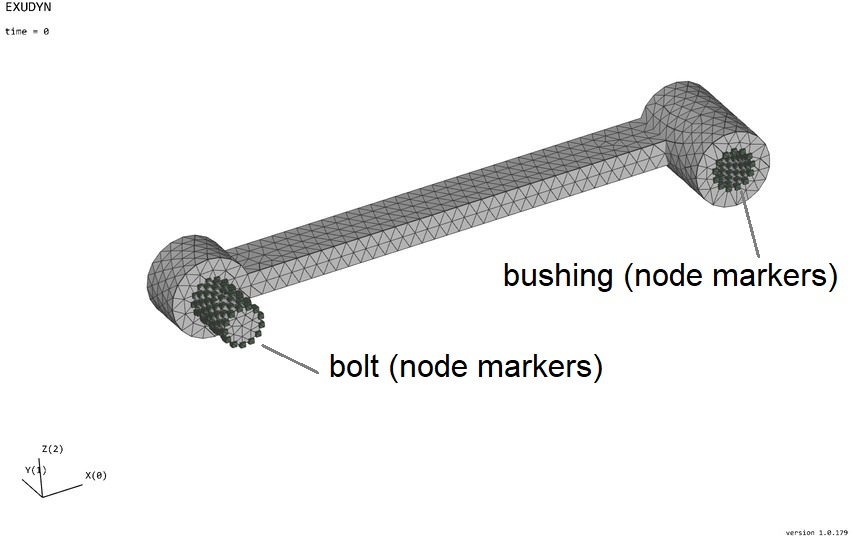
\includegraphics[width=10cm]{figures/modesHinge/HCBhingeMesh.jpg}
  %\end{center}
  %\caption{Test model and mesh for hinge created with Netgen (linear tetrahedral elements).}
  %\label{fig_hingePartMesh}
%\end{figure}
%++++++++++++++++++++++++
As an example, we consider a part denoted as 'hinge' in the following, see \fig{fig_hingePartMesh}. The test example can be found in \texttt{Examples/NGsolveCMStutorial.py} with lots of additional features.

After import of mass and stiffness matrix, eigenmodes and eigenfrequencies can be computed using \texttt{fem.ComputeEigenFrequencies(...)}, 
which computes the quantities \texttt{fem.modeBasis} and \texttt{fem.eigenValues}.
The eigenvalues in Hz can be retrieved also with the function \texttt{fem.GetEigenFrequenciesHz()}.
The function \texttt{fem.ComputeEigenFrequencies(...)} is available for dense and sparse matrices, and uses \texttt{scipy.linalg} to compute eigenvalues of the linear, undamped mechanical system
\be \label{theory:eigenmodes:EOM}
  \Mm \ddot \qv(t) + \Km \qv(t) = \fv(t) \eqDot
\ee
Here, the total number of coordinates of the system is $n$, 
thus having the vector of system coordinates $\qv \in \Rcal^n$, 
vector of applied forces $\fv \in \Rcal^n$, 
mass matrix $\Mm \in \Rcal^{n \times n}$ and stiffness matrix $\Km \in \Rcal^{n \times n}$. 
If we are interested in free vibrations of the system, without any boundary conditions or interconnections to other bodies, \eq{theory:eigenmodes:EOM} can be converted to a generalized eigenvalue problem. Using the approach 
$\qv(t) = \vv \mathrm{e}^{\mathrm{i} \omega t}$ in \eq{theory:eigenmodes:EOM}, and thus $\ddot \qv(t) = -\omega^2 \qv(t)$, we obtain
\be \label{theory:eigenmodes:harmonicEquation}
    \left[ \left(-\omega^2 \Mm + \Km \right) \vv \right] \mathrm{e}^{i\omega t} = \Null \eqDot
\ee
Assuming that \eq{theory:eigenmodes:harmonicEquation} is valid for all times, the \mybold{generalized eigenvalue problem} follows that
\be \label{theory:eigenmodes:GEP}
  \left(-\omega^2 \Mm + \Km \right) \vv = \Null \eqComma
\ee
which can be rewritten as
\be \label{theory:eigenmodes:GEP2}
  \det \left(-\omega^2 \Mm + \Km \right) = 0 \eqComma
\ee
and which defines the eigenvalues $\omega_i^2$ of the linear system, where $i \in \{0, \ldots, n-1\}$. Note that in this case, the eigenvalues are the squared eigenfrequencies (in rad/s).
We can use eigenvalue algorithms to compute the eigenvalues $\omega_i^2$ and according eigenvectors $\vv_i$ from Python.
The function \texttt{fem.ComputeEigenmodes(...)} uses \texttt{eigh(...)} from \texttt{scipy.linalg} in the dense matrix mode, 
and in the sparse mode \texttt{eigsh(...)} from \texttt{scipy.sparse.linalg}, the latter being restricted to pure symmetric matrices.
Using special shift-inverted techniques in \texttt{eigsh(...)}, it performs much better than standard settings. However, you may tune your specific eigenvalue problem by modifying the solver procedure (just copy that function and adjust to your needs).
As an output, we obtain the smallest \texttt{nModes} eigenvectors (=eigenmodes)\footnote{Eigenvectors are the result of the eigenvalue algorithm, such as the QR algorithm. The mechanical interpretation of eigenvectors are eigenmodes, that can be visualized as shown in the figures of this section.} of the system.
Here, we will also use synonymously the terms 'eigenmodes' and 'normal modes', which result from an eigenvalue/eigenvector computation using certain (or even no) boundary conditions.
%++++++++++++++++++++++++
\onlyRST{
\LatexRSTfigure{figures/freeFreeModesStress}{fig_hingePartFreeFreeModes}{16cm}{800}{Lowest 8 free-free modes for hinge finite element model, contour plot for $xx$-stress component.}
}
\ignoreRST{
\begin{figure}[tbph]
  \begin{center}
  \includegraphics[width=4cm]{figures/modesHinge/freeFreeModeStress1}
  \includegraphics[width=4cm]{figures/modesHinge/freeFreeModeStress2}
  \includegraphics[width=4cm]{figures/modesHinge/freeFreeModeStress3}
  \includegraphics[width=4cm]{figures/modesHinge/freeFreeModeStress4}\\
  \includegraphics[width=4cm]{figures/modesHinge/freeFreeModeStress5}
  \includegraphics[width=4cm]{figures/modesHinge/freeFreeModeStress6}
  \includegraphics[width=4cm]{figures/modesHinge/freeFreeModeStress7}
  \includegraphics[width=4cm]{figures/modesHinge/freeFreeModeStress8}
  \end{center}
  \caption{Lowest 8 free-free modes for hinge finite element model, contour plot for $xx$-stress component.}
  \label{fig_hingePartFreeFreeModes}
\end{figure}
}
%++++++++++++++++++++++++

Clearly, if there are no supports included in the stiffness matrix, the resulting eigenmodes will contain 6 rigid body modes and we will also call this case for the computation of eigenmodes the free-free case, in analogy to a simply supported beam.
This rigid body modes, which are usually not needed (=unwanted) in the succeeding computation, can be excluded with an according option in \vspace{6pt}\\
\texttt{fem.ComputeEigenFrequencies(excludeRigidBodyModes = ...)}
\vspace{12pt}\\
For our test example, 8 eigenmodes are shown in \fig{fig_hingePartFreeFreeModes}, where the 6 rigid body modes have been excluded (so in total, 14 eigenvectors were computed).
%free free modes (coarse mesh, nNodes= 1216):
%freq(Hz)=[ 671.59137506  707.17488417 1298.50905491 1929.97563131 1971.76505866
%3141.47119938 3595.34508711 4317.51987533]
The 8 eigenfrequencies for the chosen coarse mesh with mesh size $h=0.01$ and 1216 nodes result as 
\be
  f_{0..7} = [ 671.59, 707.17, 1298.50, 1929.97, 1971.76, 3141.47, 3595.34, 4317.51] Hz
\ee
Note, that a computation with a finer mesh, using mesh size $h=0.002$ and 100224 nodes, leads to significantly different eigenfrequencies, starting with $f_0=371.50\,$Hz. This shows that quadratic finite elements would be more appropriate for this case.

After the computation of modes, it is always a good idea to visualize and/or animate these modes. We can do this, using the function \texttt{AnimateModes(...)} available in \texttt{exudyn.interactive}, which allows us to inspect and animate modes and to create animations for these modes, see the mentioned example.

Clearly, the free-free modes in \fig{fig_hingePartFreeFreeModes} are not well suited for the modeling of the deformations within the hinge, if the bolt and the bushing shall be fixed to ground or to another part. 
%TO BE DONE:
%We investigate this by adding a simple revolute joint to the bolt.
Therefore, we can use modes based on ideas of Hurty \cite{Hurty1965} and Craig-Bampton \cite{CraigBampton1968}, as shown in the following.


%+++++++++++++++++++++++++++++++++++++++++++++++++++++++++++++++++++++++++++++++++++++++++++++++++++++++++++++++++++++++
%+++++++++++++++++++++++++++++++++++++++++++++++++++++++++++++++++++++++++++++++++++++++++++++++++++++++++++++++++++++++
%+++++++++++++++++++++++++++++++++++++++++++++++++++++++++++++++++++++++++++++++++++++++++++++++++++++++++++++++++++++++
\mysubsubsectionlabel{Hurty-Craig-Bampton modes}{sec:hurty-craig-bampton-modes}
This section will describe the computation of static and eigen (normal) modes using FEMinterface.
The theory is based on Hurty \cite{Hurty1965} and Craig-Bampton \cite{CraigBampton1968}, but often only attributed to Craig-Bampton.
Furthermore, boundaries are also called interfaces\footnote{Here, and in the description of various Python functions, we will use boundary and interface often synonymously, as flexible bodies can be either connected to ground in the sense of a classical 'support-type' boundary condition, or they can represent the boundary of the flexible body as an interface to joints (via markers).}, as they either represent surface sections of our finite element model which are connected to the ground or they represent interfaces to joints and are connected to other bodies.

The computation of so-called static and normal modes follows a simple concept based on finite element mass and stiffness matrices.
The final goal of the computation of modes is to approximate the solution $\qv \in \Rcal^n$ 
by means of a reduction basis $\tPsi \in \Rcal^{n \times m}$ 
and a reduced set of coordinates $\pv \in \Rcal^m$, for which we assume $m \ll n$.

In order to include boundary/interface effects, we separate our nodes and the nodal coordinates into 
\bi
  \item[] a) boundary nodes $\qv_b \in \Rcal^{n_b}$ and
  \item[] b) internal or inner nodes $\qv_i \in \Rcal^{n_i}$.
\ei
We assume that internal nodes are not exposed to boundary/interface conditions or to forces.

Therefore, we may rewrite \eq{theory:eigenmodes:EOM} as follows
\be \label{eq_GuyanIrons}
  \mp{\Mm_{bb}}{\Mm_{bi}}{\Mm_{ib}}{\Mm_{ii}} \vp{\ddot{\qv}_b}{\ddot{\qv}_i} + \mp{\Km_{bb}}{\Km_{bi}}{\Km_{ib}}{\Km_{ii}} \vp{\qv_b}{\qv_i} =   \vp{\fv_b}{\Null}
\ee
or, equivalently,
\bea
  \Mm_{bb} \ddot{\qv}_b + \Mm_{bi} \ddot{\qv}_i +\Km_{bb}  {\qv}_b + \Km_{bi}  {\qv}_i  = {\fv}_b \label{eq_Guyan_bb}\\
  \Mm_{ib} \ddot{\qv}_b + \Mm_{ii} \ddot{\qv}_i +\Km_{ib}  {\qv}_b + \Km_{ii}  {\qv}_i  = \Null \eqDot \label{eq_Guyan_ii}
\eea
A pure static condensation follows from \eq{eq_GuyanIrons} with the assumption that inertia terms are neglected,
leading to the static result for internal nodes,
\be 
  {\qv}_{i,stat}=-\Km_{ii}^{-1} \Km_{ib} {\qv}_{b} \eqDot 
\ee
A pure static condensation, also denoted as Guyan-Irons method, keeps boundary coordinates but removes all internal modes, using the approximation
\be
  \label{eq_guans_red}
  \vp{\qv_b}{\qv_i} \approx \vp{\Im}{-\Km_{ii}^{-1} \Km_{ib}}  \qv_b = \tPsi^{GI} \qv_b \eqComma
\ee
which leads to no approximations ('exact') results for the static case, but poor performance in highly dynamic problems.

Significant improvement result from the Hurty-Craig-Bampton method, which adds eigenmodes of the internal coordinates (internal nodes).
We assume that $\tPsi_{ii}$ is the matrix of eigenvectors as a solution to the eigenvalue problem
\be \label{theory:eigenmodes:GEPii}
  \left(-\omega^2 \Mm_{ii} + \Km_{ii} \right) \vv = \Null \eqComma
\ee
Hereafter, we will only keep the lowest (or other appropriate) $m$ eigenmodes in a reduced eigenmode matrix,
\be
  \tPsi^{(red)}_{ii} = \left[\tPsi_{ii,0}, \ldots, \tPsi_{ii,m-1} \right]
\ee
Combining these 'fixed-fixed' eigenvectors with the Guyan-Irons reduction \eqref{eq_guans_red}, we obtain the 
Hurty-Craig-Bampton modes as
\be
  \vp{\qv_b}{\qv_i} \approx \vp{\Im}{-\Km_{ii}^{-1} \Km_{ib}}  \qv_b  +  \vp{\Null}{\tPsi_{r,i}}  \pv_{r} \eqComma
\ee
or in matrix form
\be \label{theory:eigenmodes:HCB}
  \vp{\qv_b}{\qv_i} \approx \mp{\Im}{\Null}{-\Km_{ii}^{-1} \Km_{ib}}{\tPsi_{r,i}}   \vp{\qv_b}{\pv_r} = \tPsi^{HCB} \pv^{HCB} \eqDot
\ee
The disadvantage of \eq{theory:eigenmodes:HCB} is evident by the fact that there may be a large number of boundary/interface nodes, leading to a huge number of static modes (100s or 1000s) and thus making the model reduction inefficient. Therefore, we can switch to other interfaces, as described in the following.

\mysubsubsubsection{Definition of RBE2 / RBE3 interfaces}
A powerful extension, which is available in many finite element as well as flexible multibody codes, is the definition of special boundary/interface conditions, based on pure rigid body motion.
The so-called RBE2 boundaries are defined such that they are firmly connected to a rigid frame, thus the boundary or interface can only undergo rigid body motion.
The advantage of this procedure is that, in comparison to \eq{theory:eigenmodes:HCB}, the number of boundary/interface modes is given by 6 \myitalics{rigid body} modes, which allow simple integration into standard joints of multibody systems, e.g., the \texttt{GenericJoint}.
The disadvantage is that such modes usually lead to artificial stiffening and stresses close to the boundary.

For so-called RBE3 boundaries, the kinematics is significantly different. The displacement of RBE3 boundaries is the (weighted) average displacement of all boundary nodes. The resulting forces at the RBE3 boundary are equally distributed, again using node-weighting.
The (linearized) rotation of RBE3 boundaries is computed as the weighted displacements of the boundaries and including the distance to the rotation axes. 
Forces due to torques at RBE3 boundaries are computed according to the weighting, again considering the distance to the rotation axes, see the according formulas later on. The computation of RBE3 boundaries widely follows the formulation of the \texttt{MarkerSuperElementRigid}, see \refSection{sec:item:MarkerSuperElementRigid}.

\mysubsubsubsection{Computation of Hurty-Craig-Bampton modes with RBE2 interfaces}
In the following section, we show the procedure for the computation of static modes for the RBE2 rigid-body interfaces.
Note that eigenmodes directly follow from matrices $\Mm_{ii}$ and $\Km_{ii}$ as described in \refSection{sec:hurty-craig-bampton-modes}.
The implementation is given in \texttt{fem.ComputeHurtyCraigBamptonModes(...)}, see \refSection{sec:FEM:FEMinterface:ComputeHurtyCraigBamptonModes}.

First, we use the index $j$ here as a node index, having the clear correspondence to the coordinate index $i$, that node $j$ has coordinates 
$[3\cdot j,\; 3\cdot j+1,\; 3\cdot j+2]$.
Furthermore, nodes are split into boundary and internal nodes, which then leads to according internal and boundary coordinates.
We shall note that this sorting is never done in the finite element model or matrices, but just some indexing (referencing) lists are generated and used throughout, using valuable features of \texttt{numpy.linalg} and \texttt{scipy.sparse}.

For a certain boundary node set $B=[j_0, \; j_1, \; j_2, \; ...] \in \Ncal^{n_b}$ with certain $n_b$ node indices $j_0, ...$, we define one boundary set. The following transformations need to be performed for every set of boundary node lists. We also assume that weighting of all boundary nodes is equal, which may not be appropriate in all cases.

If we assume that there may only occur rigid body translation and rotation for the whole boundary node set, which is according to the idea of so-called RBE2 boundary conditions, it follows that the translation of all boundary nodes is given by
\be
  %\Tm_t = \left[ \Im \; \Im \; \ldots \; \Im \right]\tp \in \Rcal^{3 n_b \times 3}
  \Tm_t = \vr{ \Im }{ \vdots}{ \Im} \in \Rcal^{3 n_b \times 3}
\ee
with $\Im \in \Rcal^{3\times 3}$ identity matrices. 
The nodal translation coordinates on boundary $B$ are denoted as $\qv_{B,t} \in \Rcal^3$. The translation of the boundary/interface is mapped to the boundary coordinates as follows (assuming only one boundary $B$),
\be
  \qv_{b,t} = \Tm_t \, \qv_{B,t}
\ee
The nodal rotation coordinates on boundary $B$ are denoted as $\qv_{B,r} \in \Rcal^3$. The rotation of the boundary/interface is mapped to the boundary coordinates as follows (assuming only one boundary $B$),
\be
  \qv_{b,r} = \Tm_r \, \qv_{B,r}
\ee
The computation of matrix $\Tm_r$ is more involved. It is based on nodal (reference) position vectors $\rv^{(0)}_j$, $j \in B$, 
the midpoint of all boundary nodes, 
\be
  \rv^{(m)} = \frac{1}{n_b} \sum_{j=0}^{n_b-1} \rv^{(0)}_j
\ee
and the position relative to the midpoint, denoted as 
\be
  \rv_j = \rv^{(0)}_j - \rv^{(m)} \eqDot
\ee
Note that the coordinate system refers to the system used in the underlying finite element mesh.
The transformation for rotation follows from 
\be
  %in old version, j should have been 0, 1, 2, ...
  %\Tm_r  = \left[ \widetilde \tOmega_x \rv_{j_0} \;\; \widetilde \tOmega_y \rv_{j_0} \;\; \widetilde \tOmega_z \rv_{j_0} \;\;
                  %\widetilde \tOmega_x \rv_{j_1} \;\; \widetilde \tOmega_y \rv_{j_1} \;\; \widetilde \tOmega_z \rv_{j_1}
                  %\ldots \right]\tp \in \Rcal^{3 n_b \times 3}
  \Tm_r = \vr{ \tilde \rv_0 }{ \vdots}{ \tilde \rv_{n_b-1}} \in \Rcal^{3 n_b \times 3} \eqDot
\ee
%with the special tensors, representing rotation about (x,y,z)-axes,
%\be
  %\widetilde\tOmega_x = \mr{0}{0}{0} {0}{0}{-1} {0}{1}{0}, \quad
  %\widetilde\tOmega_y = \mr{0}{0}{1} {0}{0}{0} {-1}{0}{0}, \quad
  %\widetilde\tOmega_z = \mr{0}{-1}{0} {1}{0}{0} {0}{0}{0} \eqDot
%\ee
%
The total nodal coordinates at the boundary, representing translations and rotations, follow as
\be
  \qv_{B} = \vp{\qv_{B,t}}{\qv_{B,r}} \eqComma
\ee
and the transformation matrix for the translation and rotation simply reads
\be
  \Tm = [\Tm_t \;\; \Tm_r] \in \Rcal^{3n_b \times 6} \eqComma
\ee
which provides the total mapping of boundary rigid body motion
\be
  \qv_{b} = \Tm \, \qv_{B} \eqComma
\ee 
which is the sum of translation and rotation.

As an example, having the boundary nodes sorted for two boundary node set $B_0$ and $B_1$, we obtain the following transformation for the Hurty-Craig-Bampton method with only 6 modes per boundary node set,
\be \label{theory:eigenmodes:HCBRBE2}
  %\vp{\qv_b}{\qv_i} \approx \mp{ \Im \mp{\Tm_0}{}{}{\Tm_1}}{\Null}{-\Km_{ii}^{-1} \Km_{ib}\vp{\Tm_0}{\Tm_1}}{\tPsi_{r,i}}   
  %\vr{\qv_{B_0}}{\qv_{B_1}}{\pv_r} \eqDot
  \vp{\qv_b}{\qv_i} \approx \mr{ \Tm_0}{\Null}{\Null} {\Null}{\Tm_1}{\Null} 
                            {-\Km_{ii}^{-1} \Km_{ib}\vp{\Tm_0}{\Null} }{-\Km_{ii}^{-1} \Km_{ib}\vp{\Null}{\Tm_1} }{\tPsi_{r,i}}   
  \vr{\qv_{B_0}}{\qv_{B_1}}{\pv_r} \eqDot
\ee
with the new boundary node vector $\qv_b = [\qv_{B_0}\tp \;\; \qv_{B_1}\tp]\tp$.

\noindent \mybold{Notes}:
\bi
  \item The inverse $\Km_{ii}^{-1} $ is not computed, but this matrix is LU-factorized using sparse techniques.
  \item The factorization only needs to be applied to six vectors for every relevant boundary node set.
  \item One set of boundary nodes can be omitted from the final static modes in \eq{theory:eigenmodes:HCBRBE2}, because keeping all boundary modes, would introduce six rigid body motions to our mode basis, what is usually not wanted nor needed.
\ei

Using again the examples given in \fig{fig_hingePartMesh}, we now obtain a set of modified modes using the function \texttt{fem.ComputeHurtyCraigBamptonModes(...)}.
\fig{fig_hingePartStaticModesA} shows the first 6 rigid body modes. Note that these modes are automatically removed in the function \texttt{fem.ComputeHurtyCraigBamptonModes(...)} with default settings.
\fig{fig_hingePartStaticModesB} shows the second set of 6 rigid body modes. 
Finally, 8 eigenmodes have been computed for the fixed-fixed case (where all boundary/interfaces nodes are fixed),
see \fig{fig_hingePartFixedFixedModes}. 
The eigenfrequencies for this case now are significantly higher than in the free-free case, reading
\be
  f_{0..7} = [1277.35, 1469.86, 3336.91, 3584.28, ...]
\ee
%Hurty-Craig-Bampton modes (coarse mesh, nNodes= 1216):
 %freq(Hz)=[1277.35052832 1469.86514681 3336.91168906 3584.28464361 5079.65220372
 %6035.58805197 6049.99829894 6568.47108075]
%++++++++++++++++++++++++
\onlyRST{
\LatexRSTfigure{figures/HCBmodesHingeStaticA}{fig_hingePartStaticModesA}{15cm}{800}{Static modes for bolt rigid body interface, using Hurty-Craig-Bampton method; top three images show (x,y,z)-translation modes, bottom three images show (x,y,z)-rotation modes; contour color represents norm of displacements.}
\LatexRSTfigure{figures/HCBmodesHingeStaticB}{fig_hingePartStaticModesB}{15cm}{800}{Static modes for bushing rigid body interface, using Hurty-Craig-Bampton method; top three images show (x,y,z)-translation modes, bottom three images show (x,y,z)-rotation modes; contour color represents norm of displacements.}
\LatexRSTfigure{figures/HCBmodesHingeEigenmode}{fig_hingePartFixedFixedModes}{16cm}{800}{Eigenmodes for fixed-fixed case, resulting from Hurty-Craig-Bampton method; contour color represents norm of displacements.}
}
\ignoreRST{
\begin{figure}[tbph]
  \begin{center}
  \includegraphics[width=5cm]{figures/modesHinge/HCBmodesHingeStaticAx}
  \includegraphics[width=5cm]{figures/modesHinge/HCBmodesHingeStaticAy}
  \includegraphics[width=5cm]{figures/modesHinge/HCBmodesHingeStaticAz}\\
  \includegraphics[width=5cm]{figures/modesHinge/HCBmodesHingeStaticArotX}
  \includegraphics[width=5cm]{figures/modesHinge/HCBmodesHingeStaticArotY}
  \includegraphics[width=5cm]{figures/modesHinge/HCBmodesHingeStaticArotZ}
  \end{center}
  \caption{Static modes for bolt rigid body interface, using Hurty-Craig-Bampton method; top three images show (x,y,z)-translation modes, bottom three images show (x,y,z)-rotation modes; contour color represents norm of displacements.}
  \label{fig_hingePartStaticModesA}
\end{figure}
%++++++++++++++++++++++++

%++++++++++++++++++++++++
\begin{figure}[tbph]
  \begin{center}
  \includegraphics[width=5cm]{figures/modesHinge/HCBmodesHingeStaticBx}
  \includegraphics[width=5cm]{figures/modesHinge/HCBmodesHingeStaticBy}
  \includegraphics[width=5cm]{figures/modesHinge/HCBmodesHingeStaticBz}\\
  \includegraphics[width=5cm]{figures/modesHinge/HCBmodesHingeStaticBrotX}
  \includegraphics[width=5cm]{figures/modesHinge/HCBmodesHingeStaticBrotY}
  \includegraphics[width=5cm]{figures/modesHinge/HCBmodesHingeStaticBrotZ}
  \end{center}
  \caption{Static modes for bushing rigid body interface, using Hurty-Craig-Bampton method; top three images show (x,y,z)-translation modes, bottom three images show (x,y,z)-rotation modes; contour color represents norm of displacements.}
  \label{fig_hingePartStaticModesB}
\end{figure}
%++++++++++++++++++++++++

%++++++++++++++++++++++++
\begin{figure}[tbph]
  \begin{center}
  \includegraphics[width=4cm]{figures/modesHinge/HCBmodesHingeEigenmode0}
  \includegraphics[width=4cm]{figures/modesHinge/HCBmodesHingeEigenmode1}
  \includegraphics[width=4cm]{figures/modesHinge/HCBmodesHingeEigenmode2}
  \includegraphics[width=4cm]{figures/modesHinge/HCBmodesHingeEigenmode3}\\
  \includegraphics[width=4cm]{figures/modesHinge/HCBmodesHingeEigenmode4}
  \includegraphics[width=4cm]{figures/modesHinge/HCBmodesHingeEigenmode5}
  \includegraphics[width=4cm]{figures/modesHinge/HCBmodesHingeEigenmode6}
  \includegraphics[width=4cm]{figures/modesHinge/HCBmodesHingeEigenmode7}
  \end{center}
  \caption{Eigenmodes for fixed-fixed case, resulting from Hurty-Craig-Bampton method; contour color represents norm of displacements.}
  \label{fig_hingePartFixedFixedModes}
\end{figure}
%++++++++++++++++++++++++
}
\mysubsubsubsection{Computation of Hurty-Craig-Bampton modes with RBE3 interfaces}
we are currently finishing a paper, after which this section will be completed!

%+++++++++++++++++++++++++++++++++++++++++++++++++++++++++++++++++++++++++++++++++++++++
%+++++++++++++++++++++++++++++++++++++++++++++++++++++++++++++++++++++++++++++++++++++++
%synchronize this section with the paper!
%\mysubsubsubsection{Computation of Hurty-Craig-Bampton modes with RBE3 interfaces}
%In the following section, we show the procedure for the computation of static and eigenmodes for the RBE3 rigid-body interfaces.
%The implementation is given in \texttt{fem.ComputeHurtyCraigBamptonModes(...)}, see \refSection{sec:FEM:FEMinterface:ComputeHurtyCraigBamptonModes}.
%
%It shall be noted that there are slightly different versions of RBE3 modes, as there are several possibilities to define average displacements and rotations,
%and there are several ways to define the eigen-problem for eigenmodes.
%Here, we chose the following way to compute eigenmodes:
%\bi
  %\item at every boundary, which may not contain overlapping nodes with other boundaries, the weighted average displacement and the weighted average rotation is fixed by imposing 6 constraints per boundary;
  %\item for the computation of static modes, a single DOF at the rigid boundaries is prescribed with an average unit displacement or unit rotation.
  %\item for the computation of eigenmodes, all weighted displacements/rotations are fixed and eigenmodes are computed for lowest eigenfrequencies.
%\ei
%%
%The stiffness matrix, sorted for boundary and internal nodal coordinates reads, compare \eq{eq_GuyanIrons},
%\be
  %\Km = \mp{\Km_{bb}}{\Km_{bi}}{\Km_{ib}}{\Km_{ii}}
%\ee
%
%\noindent
%For every boundary $B \in [B0, B1, \ldots ]$ of $n_B$ boundaries, we defined linear constraints, using the same boundary node definitions as for RBE2 boundaries.
%The three linear constraints for average displacements are given for boundary nodes $j$ with displacement vectors $\qv_{b,j}$ and nodal weights per boundary $w_{B,j}$\footnote{note that the sum of all weights follows as $\sum_j w_{B,j}=1$.}, 
%\be
  %\cv_{b,t}(\qv_b) = \Cm_{b,t} \qv_b = \sum_{j=0}^{n_B-1} w_{B,j} \qv_{B,j} = \uv_B
%\ee
%which implicitly defines $\Cm_{b,t} \in \Rcal^{3 n_b \times 3}$, while $\Cm_{i,t} = \Null \in \Rcal^{3 n_i \times 3}$.
%The prescribed displacement $\uv_B$ is zero, except that this boundary mode is currently computed.
%
%For rotations, the nodal (reference) position vectors $\rv^{(0)}_j$, $j \in B$ and
%the midpoint of all boundary nodes, 
%\be
  %\rv^{(m)} = \frac{1}{n_b} \sum_{j=0}^{n_B-1} w_{B,j} \rv^{(0)}_j \eqComma
%\ee
%are again used to define positions relative to the midpoint $\rv^{(m)}$, 
%\be
  %\rv_j = \rv^{(0)}_j - \rv^{(m)} \eqDot
%\ee
%Note that the coordinate system refers to the system used in the underlying finite element mesh.
%Similar as in the \texttt{MarkerSuperElementRigid}, see \refSection{sec:item:MarkerSuperElementRigid}, 
%we define a total weighting for all nodal reference positions relative to the boundary's midpoint as
%\be
    %\Wm = -\sum_j  w_{B,j} \tilde \rv_j \tilde \rv_j \eqComma
%\ee
%which follows from the analogy of an inertia tensor with mass distributed equally at the boundary.
%
%The three linear constraints for average rotations follow as
%\be
  %\cv_{b,r}(\qv_b) = \Cm_{b,r} \qv_b = \sum_{j=0}^{n_B-1} w_{B,j} \tilde \rv_{B,j} \qv_{B,j}  = \ttheta_B
%\ee
%which implicitly defines $\Cm_{b,r} \in \Rcal^{3 n_b \times 3}$.
%Here, $\ttheta_B$ is a weighting matrix similar to the \texttt{MarkerSuperElementRigid},
%\be
  %\ttheta_B = \sum_{j=0}^{n_B-1} -w_{B,j} \tilde \rv_{B,j} \tilde \rv_{B,j}
%\ee
%Similarly as for translations, the prescribed rotation $\ttheta_B$ is zero, except that this boundary mode is currently computed.
%Finally, we combine translation and rotation part as 
%\be
  %\Cm_{b} = \vp{\Cm_{b,t}}{\Cm_{b,r}} \eqComma
%\ee
%and set $\Cm_{i} = \Null \in \Rcal^{3 n_i \times 6}$.
%In order to compute boundary modes, the linear system of equations reads
%\be \label{eq:theory:HCB:RBE3linearEq}
  %\mr{\Km_{bb}}{\Km_{bi}}{\Cm_{b}\tp} {\Km_{ib}}{\Km_{ii}}{\Cm_{i}\tp} {\Cm_{b}}{\Cm_{i}}{\Null} \vr{\qv_b}{\qv_i}{\tlambda} = \vr{\Null}{\Null}{\tdelta} \eqDot
%\ee
%Here, $\tlambda$ represents Lagrange multipliers which represent the boundary forces and torques at the according boundaries due to unit displacements or rotations, given by the vector $\tdelta$.
%In order to compute the $k^\mathrm{th}$ boundary mode as $\vp{\qv_b^k}{\qv_i^k}$, we set the $k^\mathrm{th}$ component of $\tdelta$ to
%\be
  %\tdelta_k = 1 \eqComma
%\ee
%while all other components of $\tdelta$ are $0$ and solve \eq{eq:theory:HCB:RBE3linearEq}. This way allows to compute all static modes using a single factorization in \eq{eq:theory:HCB:RBE3linearEq} to compute all modes for all boundaries.
%
%The computation of eigenmodes require to apply all constraints to the stiffness and mass matrices, which is done by means of projection of the linear equations of motion into the null space of the constraints.
%We compute the singular value decomposition for every constraint matrix $\Cm_{b}$,
%\be
  %[\Um, \sv, \Vm] = \mathrm{SVD}(\Cm_{b}), \eqComma
%\ee
%where $\Um$ is a unitary matrix with left singular vectors as columns, $\sv$ stores singular values in the diagonal, and $\Vm$ is a 
%unitary matrix with right singular vectors as rows.
%The null space of the constraint matrix $\Cm_{b}$ is spanned by $\Vm_N \in \Rcal^{(3 n_b-6) \times 3 n_b}$, which results from $\Vm$ when removing the first 6 rows. 
%Combining the null space matrix with a unit matrix for the internal nodes, $\Im_{ii} \in \Rcal^{n_i \times n_i}$,
%the projection matrix results as
%\be
  %\Vm_P = \mp{\Vm_N}{}{}{\Im_{ii}}
%\ee
%Using the projected stiffness and mass matrices,
%\be
  %\Mm_P = \Vm_P \mp{\Mm_{bb}}{\Mm_{bi}}{\Mm_{ib}}{\Mm_{ii}} \Vm_P\tp \quad \mathrm{and} \quad
  %\Km_P = \Vm_P \mp{\Km_{bb}}{\Km_{bi}}{\Km_{ib}}{\Km_{ii}} \Vm_P\tp 
%\eqComma
%\ee
%the eigenvalue problem for the constrained system of \eq{eq:theory:HCB:RBE3linearEq} is given by
%\be \label{eq:theory:HCB:RBE3eigen}
  %\Mm_P \ddot{\qv}_P + \Km_P \qv_P = \Null \eqDot
%\ee
%The eigen analysis of \eq{eq:theory:HCB:RBE3eigen} results in the eigenvector matrix $\tPsi_P \in \Rcal^{(n-6) \times m}$, containing a set of $m$ eigenvectors.
%The final eigenvectors $\tPsi \in \Rcal^{n \times m}$ are computed by means of projection onto the original boundary nodes, using
%\be
  %\tPsi = \Vm_P\tp \tPsi_P \eqDot
%\ee
%Note that for efficiency reasons operations such as in \eq{eq:theory:HCB:RBE3eigen} are only performed for boundary nodes, but not for internal nodes.
%Furthermore, sparse matrices are used whenever matrices are large and not fully populated.
%


%+++++++++++++++++++++++++++++++++++++++++++++++++++++++++++++++++++++++++++++++++++++++
\mysubsubsectionlabel{Computation of stresses and strains for CMS modes}{sec:theory:CMS:stresses}
%
The computation of stresses and strains is not directly possible if only knowing nodal displacements, stiffness matrix and mass matrix.
In the following, we assume that we have a vector of nodal displacements $\qv$, reduced coordinates $\pv^{R}$, as well as a reduction matrix $\tPsi^{R}$, compare \eq{theory:eigenmodes:HCB},
\be \label{theory:eigenmodes:HCB2}
  \qv \approx \tPsi^{R} \pv^{R} \eqDot
\ee
Knowing all nodal displacements of a finite element allows to compute displacement, stress, and strain field within the element. This procedure is usually done within the finite element codes.
In particular, one should know that stress and strain quantities are having a lower order of accuracy than displacements and they may be more accurate in certain points, e.g., integration points. Furthermore, stress and strain quantities may have jumps along element boundaries, which is why they are usually post-processed in order to at least look smoother but in general also are more accurate.

In \codeName, we have the option to pre-compute stress or strain components at finite element nodes, see the options below.
Due to the fact that the FFRF / CMS formulation is assuming small (linearized) strains only, we are able to superimpose stress and strain for each mode. Independently of the quantity we intend to compute (stress, strain or similar), we use post-processing modes, which allow to represent special output variables.

Having a modal coordinate $\pv^{R}_k$, we define a post-processing mode (pm) such that
\be
  \sv_k^{\mathrm{pm}} = \tPsi^{\mathrm{pm}}_k \pv^{R}_k \eqComma
\ee
in which $\sv_k^{\mathrm{pm}}$ represents for example the stress component $\sigma_\mathrm{xx}$ for the mode $k$.
Putting together all stress modes for $\sigma_\mathrm{xx}$, $\sigma_\mathrm{yy}$, $\sigma_\mathrm{zz}$, $\sigma_\mathrm{yz}$, $\sigma_\mathrm{xz}$, and $\sigma_\mathrm{xy}$, 
\be
  \tPsi^{\sigma_\mathrm{xx}} = \left[\tPsi^{\sigma_\mathrm{xx}}_0, \tPsi^{\sigma_\mathrm{xx}}_1, \ldots,
               \tPsi^{\sigma_\mathrm{xx}}_{m-1}\right] \eqComma
\ee
we are able to compute $\sigma_\mathrm{xx}$ for all nodes from the relation
\be
  \sv^{\sigma_\mathrm{xx}} = \tPsi^{\sigma_\mathrm{xx}} \pv^{R}
\ee
Using the \texttt{FEMinterface} member \texttt{postProcessingModes}, the \texttt{FEM} module, we can define the \texttt{matrix} as $\tPsi^{\sigma_\mathrm{ij}}$ for every node of the finite element mesh. In particular, one has to store all stress (or strain) components consecutively for each mode, which means that for mode $k$, $\tPsi$ contains the columns
\be
  \tPsi^{\sigma}_k = \left[\tPsi^{\sigma_\mathrm{xx}}_k, \tPsi^{\sigma_\mathrm{yy}}_k, 
                           \tPsi^{\sigma_\mathrm{zz}}_k, \tPsi^{\sigma_\mathrm{yz}}_k, 
                           \tPsi^{\sigma_\mathrm{xz}}_k, \tPsi^{\sigma_\mathrm{xy}}_k\right] \eqComma
\ee
For more details, see the \texttt{FEM} module in \refSection{sec:FEM:FEMinterface:__init__}, either for function \texttt{ComputePostProcessingModes} or \texttt{ComputePostProcessingModesNGsolve}.

In order to retrieve modes, we currently have three options:
\bi
  \item Re-compute stress or strain quantities for given material parameters from nodal displacements for linear tetrahedral elements (Tet4), using the function \texttt{ComputePostProcessingModes} within the \texttt{FEM} module. This function is implemented in Python and therefore comparatively slow.
  \item For NGsolve models, you can use the \texttt{ComputePostProcessingModesNGsolve}, which takes the finite element space and material to compute post-processing modes directly in NGsolve, which is comparatively fast, if you do not have an excessive amount of modes and nodes.
  \item You can compute the post-processing modes within your finite element tool, such as Ansys or Simulia(ABAQUS) and import them manually. There exists no functionality in \codeName to do so.
\ei
In general, one should know that the size of postprocessing modes may be huge. If you have $200\,000$ nodes and 100 modes, the matrix $\tPsi^{\sigma}$ would have the size $200\,000 \times (6 \cdot 100)$, thus leading to $120\,000\,000$ components, close to 1GB of memory. In other words, it could make sense to consider computation of stresses in a post-computing phase.

%+++++++++++++++++++++++++++++++++++++++++++++++++++++++++++++++++++++++++++++++++++++++
\mysubsubsectionlabel{Interfaces and boundaries}{sec:theory:CMS:interfaces}
Being able to model a sole flexible body is not sufficient for the modeling of industrial problems.
An important part of component mode synthesis is the appropriate definition of boundaries or interfaces.
The term interface is widely used and may be more appropriate when connecting two bodies via such interfaces.
However, in some cases the flexible body may be fixed to ground via such a boundary. In order to distinguish boundary/interface (b) and internal nodes (i), boundary seems to be appropriate and boundary/interface will be used synonymously in the context of flexible bodies.

An boundary/interface is represented by a certain surface area of a body, usually defined by surface elements and underlying nodes.
For simplicity, it may just be defined by means of a node set.
This is sufficient, in order for most of the previously described algorithms to work.
If node sets are not imported from the underlying finite element codes, practical functions exist for the definition of
node sets from geometrical operations, specifically\footnote{Note that these functions perform a linear search in the whole mesh, which is computationally inefficient if it is called many times.}:
\bi
  \item \texttt{GetNodeAtPoint}: returns node number of a single node (if found) at given spatial position, with certain tolerance
  \item \texttt{GetNodesInPlane}: returns all nodes lying on a defined plane with certain tolerance
  \item \texttt{GetNodesInCube}: returns all nodes lying in a axis-parallel cube
  \item \texttt{GetNodesOnLine}: returns all nodes lying on a line defined by two points, with certain tolerance
  \item \texttt{GetNodesOnCylinder}: returns all nodes lying on a cylinder defined by two points and radius, with certain tolerance
  \item \texttt{GetNodesOnCircle}: returns all nodes lying on a circle defined by point, normal and radius, with certain tolerance
\ei
In order to compute according weighting factors, surface elements need to exist, either importing them the finite element code, or by using the \texttt{FEMinterface} member \texttt{surface}.
The surface of tetrahedral or hexahedral meshes, which follow a standard node numbering, can be computed using
the \texttt{FEMinterface} function \texttt{VolumeToSurfaceElements}.


%+++++++++++++++++++++++++++++++++++++++++++++++++++++++++++++++++++++++++++++++++++++++
\mysubsubsectionlabel{Node weighting}{sec:theory:CMS:nodeWeighting}
%
As mentioned in the literature \cite{HeirmanDesmet2010}, there are certain advantages to use regular meshes on boundaries/interfaces.
However, industrial relevant geometries often cannot be meshed by regular hexahedral meshes which leads to unstructured tetrahedral elements with (nearly) arbitrary triangular surfaces.
While being a more general approach, an according nodal weighting is inevitable for unstructured surface meshes.
As a drawback, accurate nodal weighting for application of forces or for computation of average displacements or rotations requires the information of underlying finite element interpolation functions, which are avoided in the present approach.
A simplified, first order accurate functionality is provided by \texttt{GetNodeWeightsFromSurfaceAreas}, which reconstructs nodal weights for a set of node numbers from a given triangulated surface in \texttt{FEMinterface}.
After identification of surface triangles and computation of according triangle areas, the weight $w_i$ of every node $i$ is built upon the according area of all connected triangles $j$,
\be
  w_i = \frac{1}{3 A_B} \sum_{j} A_j  \eqComma \quad \mathrm{and} \quad \sum_i w_i = 1
\ee
using the total area $A_B$ of the boundary. 
This weighting leads to nearly constant strain distribution along the cross section of a fixed bar with equally distributed axial forces.

%+++++++++++++++++++++++++++++++++++++++++++++++++++++++++++++++++++++++++++++++++++++++
\mysubsubsectionlabel{Reference conditions}{sec:theory:CMS:referenceConditions}
%
Currently, there is no specific functionality to define reference conditions for \ac{FFRF} objects in \codeName.
In the \texttt{ObjectFFRF}, a \texttt{ObjectConnectorCoordinateVector} needs to be used to define constraints of a so-called Tisserand frame.

In the \texttt{ObjectFFRFreducedOrder}, there are in general two approaches:
\bi
  \item The computed modes do not include rigid body motions, by using the appropriate flag\\ \texttt{excludeRigidBodyModes = True}\\ for most of such functions; in this case, the reference conditions are defined such that the reference node positions of the mesh are rigidly attached to the reference frame. In case of Hurty-Craig-Bampton modes, one boundary set (the first one) is attached to the reference frame.
  \item Alternatively, \texttt{excludeRigidBodyModes} can be set False, or arbitrary modes can be imported from elsewhere.
    In this case, rigid body motion must be excluded by appropriate constraints, e.g., a \texttt{ObjectConnectorCoordinateVector} applied to the \texttt{NodeGenericODE2} of \texttt{ObjectFFRFreducedOrder}. This task is completely left to the user.
\ei
It should be noted that regarding efficiency or highest accuracy, better reference conditions may exists, which are not fully supported in the current code and may only be applied with user functions.




















%RST files only considered up to here
%%RSTCOMPATIBLE


\clearpage
%+++++++++++++++++++++++++++++++++++++++++++++++++++++++++++++++++
\mysubsectionlabel{Modeling of Contact in \codeName }{secContactTheory}
% 
The \texttt{GeneralContact} module, see \refSection{sec:GeneralContact},  which is 
\bi
  \item[] \mybold{still under developement, consider with care!}
\ei
provides a simple, efficient and versatile interface to a general contact module. The movivation for this module is based on the need for simple contact modeling in robotics, but also for the efficient modeling of beam-cylinder or beam-beam contact, as well as contact between deformable meshes (not yet available).

Note that there are currently only simplistic contact models, such as linear contact and simple damping, which are not representing realistic Hertzian contact (which will be implemented in near future). Furthermore, read the notes in \texttt{GeneralContact} carefully, how stiffness and damping is realized -- e.g., stiffness may be a serial spring against the other object, while damping is implemented as parallel damper.

%++++++++++++++++++++++++++++++++++++++++++++++++++++++++++++++++++++++++
\begin{figure}[hb]
  \centering
  \begin{tikzpicture}[node distance = 2cm, auto, thick,scale=0.7, every node/.style={scale=0.7}]
      % Place nodes
      \node [cloud] (availableContacts) {\mybold{available contacts}};
      \node [wideblock, below of=availableContacts, node distance=3cm, xshift = -7.5cm] (sphericalContact) {sphere--sphere, circle--circle};
      \node [wideblock, right of=sphericalContact, node distance=4.5cm] (clusteredSphericalContact) {clustered sphere--\{sphere,trig\}};
      \node [wideblock, right of=clusteredSphericalContact, node distance=4.5cm] (sphereTrigContact) {sphere--triangle};
      \node [wideblock, right of=sphereTrigContact, node distance=4.5cm] (trigTrigContact) {triangle--triangle};
      \node [wideblock, right of=trigTrigContact, node distance=4.5cm] (circleCableContact) {circle--ANCFCable2D};
      \path [line] (availableContacts) -- (sphericalContact);
      \path [line] (availableContacts) -- (clusteredSphericalContact);
      \path [line] (availableContacts) -- (sphereTrigContact);
      \path [line] (availableContacts) -- (trigTrigContact);
      \path [line] (availableContacts) -- (circleCableContact);
  \end{tikzpicture}
  \caption{Contact: possible coupling of geometrical objects in \codeName}
  \label{fig_available_contact}
\end{figure}
%++++++++++++++++++++++++++++++++++++++++++++++++++++++++++++++++++++++++
%

\noindent \fig{fig_available_contact} shows the implemented / possible coupling of contact objects:
\bi
  \item[1)] simulate spherical particles; in 2D, spheres are represented as circles
  \item[2)] simulate clustered spherical [circular] particles which consist of rigid bodies made of a cluster of spheres; several contact spheres are attached to one rigid body by using rigid body markers; in 2D, spheres are represented as circles
  \item[3)] simulate the contact of spheres with triangular meshes, e.g., in order to provide some limitations of the range of motion for your objects
  \item[4)] simulate the contact between arbitrarily shaped rigid bodies
  \item[5)] simulate the contact between rolls (spheres) and ANCF cable elements; to enable cable-cable contact, spheres must be attached and distributed along the cable elements
\ei
In all use cases, explicit integrators are much faster and they are recommended, as long as your problem allows to do so.
%
\mysubsubsection{Contact of meshed rigid bodies}
Case 4) is more involved and needs further explanations (which more or less also applies to case 4). The geometry is approximated by a mesh consisting of flat triangles, which are attached to a rigid body (marker). The triangles obtain a contact stiffness against spheres. There are special cases, depending if the sphere gets in contact with the triangle plane or with the triangle edge. Having contact with edges, usually involves several triangles at the same time (specifically at vertices), which leads to higher contact stiffness as compared to a planar contact. Nevertheless, for flat planes, contact computation takes care, that contact stiffness is constant in the whole plane, independently of the number of involved triangles.
In order to realize contact between meshed rigid bodies, both body-attached meshes are added via the \texttt{GeneralContact} function 
\bi
  \item \texttt{AddTrianglesRigidBodyBased(...)}
\ei
In addition, all mesh vertices are added as spheres with markers using 
\bi
  \item \texttt{AddSphereWithMarker(...)}
\ei
However, as we need a certain finite radius of the spheres, the mesh must be shrinked for this purpuse (and it needs to have according thickness). Shrinking of the (consistent) triangular mesh can be done by the utility function 
\bi
  \item \texttt{ ShrinkMeshNormalToSurface(...)};
  \item in order to reduce artifacts at object edges, it is recommended to refine the mesh, using the utility function \texttt{RefineMesh(...)}
\ei
According examples can be found in test models, but there will be a more convenient function for contact of meshes attached to rigid bodies in the future.

All contacts can be created in a \texttt{GeneralContact} object -- which is not a regular object in mbs -- created by
\bi
  \item \texttt{gContact = mbs.AddGeneralContact()}
\ei
Note that one can create several, independent contact objects.
Hereafter, spheres, triangles, ... are added with appropriate functions, see \refSection{sec:GeneralContact}.
Note that triangles need to be correctly numbered (see correct normals in \fig{fig:triangleNormals}), %in GraphicsData section!
which defines inside/outside of a triangluar mesh.

\mysubsubsection{Regularized friction}
Within a regularized friction law, similar to a well known law attributed to Haff-Werner, the friction force $\fv_f$ is computed from static (dry) friction coefficient $\mu_s$ and the friction regularization velocity\footnote{global regularization coefficient stored in \texttt{GeneralContact.frictionProportionalZone}} $v_{\mu,reg}$
\bea \label{eq_GeneralContactRegularizedFriction}
  v_t &=& |\LU{0}{\vv_t}|, \nonumber \\
  \fv_f(v_t, |f_c|, \mu_s, v_{\mu,reg}, v_t, \LU{0}{\vv_t} ) &=& 
  \begin{cases}
    \frac{\mu_s \cdot |f_c|}{v_{\mu,reg}}\LU{0}{\vv_t}, \quad \mathrm{if} \quad v_t < v_{\mu,reg} \\
%    
    \mu_s \cdot |f_c| \frac{\LU{0}{\vv_t}}{v_t} , \quad \mathrm{else} 
  \end{cases}
\eea
%
\mybold{Note} that the following equations represent the computed contact relations in high detail, but minor cases and flags, such as the \texttt{intraSpheresContact} are not described here, but must be carefully considered in the description of \texttt{GeneralContact}, see \refSection{sec:GeneralContact}.

%++++++++++++++++++++++++++++++++++++++++++++++++++++++++++++++++++++++++
%++++++++++++++++++++++++++++++++++++++++++++++++++++++++++++++++++++++++
%
\mysubsubsectionlabel{Sphere-sphere contact: Equations}{secContactSphereSphere}
%
The contact model between two spheres follows a penalty formulation, using a spring and optional damper to model the contact.
Currently, only linear springs are utilized, however, the user is free to modify the equations in the code to model any nonlinear case as well.
The equations for sphere-sphere contact in contact normal direction are very similar to the \texttt{ObjectConnectorSpringDamper}, see \refSection{sec:item:ObjectConnectorSpringDamper}.
%
Every sphere is attached to a position-based marker \footnote{which can be attached itself to position nodes, rigid body nodes, point masses, rigid bodies as well as flexible bodies. NOTE, that in case of implicit integration, flexible bodies are not fully implemented!}.
%
In C++, the sphere attached to marker 0 is denoted as \texttt{sphereI} and 
the sphere attached to marker 1 is denoted as \texttt{sphereJ}.
%
Input parameters for this contact model are
\startTable{intermediate variables}{symbol}{description}
\rowTable{sphere $i$ radius}{$r_i$}{radius of sphere $i$, attached to marker 0}
\rowTable{sphere $j$ radius}{$r_j$}{radius of sphere $j$, attached to marker 1}
\rowTable{sphere $i$ contact stiffness}{$k_i$}{N/m}
\rowTable{sphere $j$ contact stiffness}{$k_j$}{N/m}
\rowTable{sphere $i$ contact damping}{$d_i$}{N/m}
\rowTable{sphere $j$ contact damping}{$d_j$}{N/m}
\rowTable{friction pairing coefficient}{$\mu_{ij}$}{the friction coefficient stored in the the friction pairings matrix, resulting from the friction indices of spheres $i$ and $j$}
\finishTable

Marker positions and velocities are given by the relations:
\startTable{intermediate variables}{symbol}{description}
\rowTable{sphere $i$ position}{$\LU{0}{\pv}_{m0}$}{current global position which is provided by marker m0}
\rowTable{sphere $j$ position}{$\LU{0}{\pv}_{m1}$}{current global position which is provided by marker m1}
\rowTable{marker m0 position Jacobian}{$\LU{0}{\Jm_{pos,m0}}$}{with interpretation as variation of the position $\delta \LU{0}{\pv}_{m0} = \LU{0}{\Jm_{pos,m0}} \delta \qv_{m0}$; assuming that $\qv_{m0}$ represents the generalized coordinates of marker $m0$}
\rowTable{marker m1 position Jacobian}{$\LU{0}{\Jm_{pos,m1}}$}{with interpretation as variation of the position $\delta \LU{0}{\pv}_{m1} = \LU{0}{\Jm_{pos,m1}} \delta \qv_{m1}$; assuming that $\qv_{m0}$ represents the generalized coordinates of marker $m0$}
\rowTable{sphere $i$ velocity}{$\LU{0}{\vv}_{i}$}{current global velocity which is provided by marker m0}
\rowTable{sphere $j$ velocity}{$\LU{0}{\vv}_{j}$}{}
\rowTable{relative position}{$\LU{0}{\nv}$}{$\LU{0}{\pv}_{j} - \LU{0}{\pv}_{i}$}
%\rowTable{relative velocity$^*$}{$\Delta\! \LU{0}{\vv}$}{$\LU{0}{\vv}_{m1} - \LU{0}{\vv}_{m0}$}
\rowTable{Distance$^*$}{$L = |\LU{0}{\nv}|$}{}
\rowTable{unit vector$^*$}{$\LU{0}{\nv_0} = \frac{1}{L} \LU{0}{\nv}$}{vector in contact normal direction}
\rowTable{gap$^*$}{$g = L - (r_i + r_j)$}{}
\rowTable{penetration$^*$}{$p  = -g = r_i + r_j - L$}{}
\finishTable

In case of rigid bodies and non-zero friction, we also compute angular velocities and orientation,
\startTable{intermediate variables: rigid bodies and friction}{symbol}{description}
\rowTable{sphere $i$ angular velocity}{$\LU{m0}{\tomega}_{i}$}{current local angular velocity provided by marker $m0$}
\rowTable{marker $m0$ orientation}{$\LU{0,m0}{\Am}$}{transformation from marker m0 (body-fixed) to global coordinates}
\rowTable{sphere $j$ angular velocity}{$\LU{m1}{\tomega}_{j}$}{current local angular velocity provided by marker $m1$}
\rowTable{marker $m1$ orientation}{$\LU{0,m1}{\Am}$}{transformation from marker m0 (body-fixed) to global coordinates}
\rowTable{marker $m0$ rotation Jacobian}{$\LU{0}{\Jm_{rot,m0}}$}{with interpretation as derivative of the global angular velocity $\LU{0}{\tomega}_{m0} = \LU{0}{\Jm_{rot,m0}} \dot \qv_{m0}$; assuming that $\dot \qv_{m0}$ represents the generalized velocities of marker $m0$}
\rowTable{marker $m1$ rotation Jacobian}{$\LU{0}{\Jm_{rot,m1}}$}{with interpretation as derivative of the global angular velocity $\LU{0}{\tomega}_{m1} = \LU{0}{\Jm_{rot,m1}} \dot \qv_{m1}$; assuming that $\dot \qv_{m1}$ represents the generalized velocities of marker $m1$}
\finishTable

%
%
\noindent Contact between spheres with global index $g_i$ and another sphere with global index $g_j$ is active, if
\bi
  \item Bounding box of sphere $g_j$ intersects with a box in the searchtree which also intersects with bounding box of sphere $g_i$ AND
  \item if Bounding box of sphere $g_j$ intersects with bounding box of sphere $g_i$ AND
  \item if the condition $L^2 < \left(r_i + r_j\right)^2$ holds OR
  if $g_j$ belongs to the active set of $g_i$ (computed in PostNewtonStep).
\ei
Note that quantities $^*$ are only computed if contact is active.

\mysubsubsubsection{Contact relations for sphere $g_i$ (marker $m0$) and sphere $g_j$ (marker $m1$)}
\noindent If contact is active, we compute the global position of the contact point\footnote{considering also penetration, a more consistent contact point would be $\LU{0}{\pv_{c}^*} = \LU{0}{\pv_{m0}} + (r_i - \frac{p}{2}) \cdot \nv_0$, subtracting the half penetration.}, see \fig{fig_GeneralContactSpheres},\footnote{note that we have to consider the penetration when computing the contact points, attributing penetration equally to both sides; we introduce therefore the modified radii $r_i^* = r_i-\frac{p}{2}$ and $r_j^* = r_j-\frac{p}{2}$.}
\be
  \LU{0}{\pv_{c}} = \LU{0}{\pv_{m0}} + r_i^* \cdot \nv_0 \eqComma
\ee
%++++++++++++++++++++++++
\begin{figure}[tbp]
  \begin{center}
  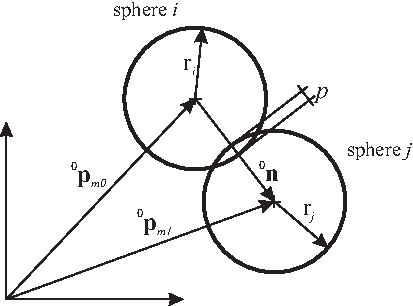
\includegraphics[width=8cm]{figures/generalContactSpheres}
  \end{center}
  \caption{Geometrical relations for contact of two spheres $i$ and $j$ with according markers $m0$ and $m1$.}
  \label{fig_GeneralContactSpheres}
\end{figure}
%++++++++++++++++++++++++
the velocities of the spheres at the contact point\footnote{In case of no friction, the angular velocities are not included in these relations},
\bea
  \LU{0}{\vv_{c,i}} &=& \LU{0}{\vv_i} + \left( \LU{0,m0}{\Am} \LU{m0}{\tomega}_{i} \right) \times 
               \left( \LU{0}{\pv_c} - \LU{0}{\pv_i} \right)
              = \LU{0}{\vv_i} + r_i^* \cdot \left( \LU{0,m0}{\Am} \LU{m0}{\tomega}_{i} \right) \times \LU{0}{\nv_0},\nonumber \\
  \LU{0}{\vv_{c,j}} &=& \LU{0}{\vv_j} + \left( \LU{0,m1}{\Am} \LU{m1}{\tomega}_{j} \right) \times 
               \left( \LU{0}{\pv_c} - \LU{0}{\pv_j} \right)
              = \LU{0}{\vv_j} - r_j^* \cdot \left( \LU{0,m1}{\Am} \LU{m1}{\tomega}_{j} \right) \times \LU{0}{\nv_0},
\eea
the velocity in contact normal direction, which can be computed from sphere's center points, 
\be
  v_n = \LU{0}{\nv_0\tp} \left( \LU{0}{\vv_j} - \LU{0}{\vv_i} \right)
      = \LU{0}{\nv_0\tp} \left( \LU{0}{\vv_{c,j}} - \LU{0}{\vv_{c,i}} \right)
  \eqComma
\ee
the velocity in tangential direction, considering the tangential velocities,
\bea
  \LU{0}{\vv_t} &=& \LU{0}{\vv_{c,j}} - \LU{0}{\vv_{c,i}} - v_n \cdot \LU{0}{\nv_0} 
  = \left( \Im - \LU{0}{\nv_0} \otimes \LU{0}{\nv_0}\right) \left(\LU{0}{\vv_{c,j}} - \LU{0}{\vv_{c,i}} \right), \nonumber \\
  &=& \left( \Im - \LU{0}{\nv_0} \otimes \LU{0}{\nv_0}\right) 
  \left( \LU{0}{\vv_j} + r_j^* \cdot \LU{0}{\tilde \nv_0} \LU{0,m1}{\Am} \LU{m1}{\tomega}_{j} 
        -\LU{0}{\vv_i} + r_i^* \cdot \LU{0}{\tilde \nv_0} \LU{0,m0}{\Am} \LU{m0}{\tomega}_{i} \right) \nonumber \\
  &=& \left( \Im - \LU{0}{\nv_0} \otimes \LU{0}{\nv_0}\right) 
  \left( \LU{0}{\vv_j} + r_j^* \cdot \LU{0}{\tilde \nv_0} \LU{0}{\tomega}_{j} 
        -\LU{0}{\vv_i} + r_i^* \cdot \LU{0}{\tilde \nv_0} \LU{0}{\tomega}_{i} \right)
  \eqComma
\eea
the effective contact stiffness coefficient based on the stiffness $k_i$ of sphere $i$ and stiffness $k_j$ of sphere $j$,
\be
  k_c = \frac{k_i \cdot k_j}{k_i + k_j} \eqComma
\ee
and the effective contact damping coefficient\footnote{Note that this simplicial damping law is used according to the idea of parallel dampers, because serial dampers would not allow to adjust damping for different particles} based on the damping $k_i$ of sphere $i$ and damping $k_j$ of sphere $j$
\be
  d_c = d_i + d_j \eqDot
\ee
The contact force (negative contact pressure) is computed from gap $g$ and normal velocity $v_n$,
\be
  f_c = k_c \cdot g + d_c \cdot v_n \eqComma
\ee
and the total vectorial contact force is computed with the help of \eq{eq_GeneralContactRegularizedFriction}, defining the friction force $\fv_f(v_t, |f_c|, \mu_s, v_{\mu,reg}, v_t, \LU{0}{\vv_t} )$,
\be
  \LU{0}{\fv_c} = f_c \cdot \nv_0 + \fv_f
  \eqDot
\ee
The torque due to friction for sphere $i$ and sphere $j$ results into\footnote{note that both signs are the same and that $\LU{0}{\fv_f}$ could be replaced by $\fv_c$}
\be
  \LU{0}{\ttau_{f,i}} = (-r_i^* \cdot \nv_0) \times \LU{0}{\fv_f}, \quad
  \LU{0}{\ttau_{f,j}} = (-r_j^* \cdot \nv_0) \times \LU{0}{\fv_f}
  \eqDot
\ee
%+++++++++++++++++++++++++++++++++++++++++++++++++++
\mysubsubsubsection{Generalized forces due to contact}
Based on the contact pressure and the friction forces, forces and torques are applied via the markers' Jacobians, resulting in generalized forces to whatever the marker is attached to.

The generalized forces to the marker $m0$ and $m1$ (sphere $i$ and $j$) are computed as
\bea
  \fv_{m0,LHS} = -\LU{0}{\Jm_{pos,m0}\tp} \LU{0}{\fv_c} + 
                 \LU{0}{\Jm_{rot,m0}\tp} \LU{0}{\ttau_{f,i}}, \nonumber \\
  \fv_{m1,LHS} = \LU{0}{\Jm_{pos,m1}\tp} \LU{0}{\fv_c} + 
                 \LU{0}{\Jm_{rot,m1}\tp} \LU{0}{\ttau_{f,j}} \eqDot
\eea
%+++++++++++++++++++++++++++++++++++++++++++++++++++
\mysubsubsubsection{Jacobi matrix for sphere $g_i$ and sphere $g_j$}
%
%
For implicit time integration, the (contact) Jacobian\footnote{Here, we only consider the local Jacobian related to the coordinates underlying the two markers $m0$ and $m1$; in the implementation, the parts of the Jacobian are added to the sparse system } represents the derivative of the generalized forces 
\be
  \fv_{LHS} = \vp{\fv_{m0,LHS}}{\fv_{m1,LHS}}
\ee
with respect to the generalized coordinates affected by the two markers,
\be
  \qv = \vp{\qv_{m0}}{\qv_{m1}} \eqDot
\ee
The Jacobian thus reads\footnote{\mybold{NOTE} that only terms marked in \mybold{\termC{green}} are currently fully implemented and terms in \mybold{\termA{blue}} are approximated, while other terms are neglected}
\be
  \termA{ \Jm_{c}  = \frac{\partial \fv_{LHS}}{\partial \qv}
           = \mp{\frac{\partial \left(-\LU{0}{\Jm_{pos,m0}\tp} \LU{0}{\fv_c} + \LU{0}{\Jm_{rot,m0}\tp} \LU{0}{\ttau_{f,i}}\right)}{\partial \qv_{m0}}}
                {\frac{\partial \left(-\LU{0}{\Jm_{pos,m0}\tp} \LU{0}{\fv_c} + \LU{0}{\Jm_{rot,m0}\tp} \LU{0}{\ttau_{f,i}}\right)}{\partial \qv_{m1}}}
                {\frac{\partial \left( \LU{0}{\Jm_{pos,m1}\tp} \LU{0}{\fv_c} + \LU{0}{\Jm_{rot,m1}\tp} \LU{0}{\ttau_{f,j}}\right)}{\partial \qv_{m0}}}
                {\frac{\partial \left( \LU{0}{\Jm_{pos,m1}\tp} \LU{0}{\fv_c} + \LU{0}{\Jm_{rot,m1}\tp} \LU{0}{\ttau_{f,j}}\right)}{\partial \qv_{m1}}}}
\ee
The single terms may be expressed as
%terms with $\diamond$ are neglected in the current implementation}
\bea
  &&\termA{\frac{\partial \left(-\LU{0}{\Jm_{pos,m0}\tp} \LU{0}{\fv_c} + \LU{0}{\Jm_{rot,m0}\tp} \LU{0}{\ttau_{f,i}}\right)}{\partial \qv_{m0,1}} } = \nonumber \\
  &&-\frac{\partial \LU{0}{\Jm_{pos,m0}\tp}}{\partial \qv_{m0,1}} \LU{0}{\fv_c}
  \termC{-\LU{0}{\Jm_{pos,m0}\tp}} \termA{\frac{\partial \LU{0}{\fv_c}}{\partial \qv_{m0,1}}}
  +\frac{\partial \LU{0}{\Jm_{rot,m0}\tp}}{\partial \qv_{m0,1}} \LU{0}{\ttau_{f,i}}
  +\termC{\LU{0}{\Jm_{rot,m0}\tp}} \termA{\frac{\partial \LU{0}{\ttau_{f,i}}}{\partial \qv_{m0,1}}}
  \eqComma
\eea
and similar for $m_1$.
In order to simplify implementation (avoiding arrays with 3 indices) and improve computational efficiency, 
derivatives of Jacobians are realized as
\be
  \frac{\partial \LU{0}{\Jm_{pos,m0}\tp}}{\partial \qv_{m0}} \LU{0}{\fv_c} = 
  \frac{\partial \LU{0}{\Jm_{pos,m0}\tp} \LU{0}{\bar \fv_c}}{\partial \qv_{m0}}  
  \eqComma
\ee
in which $\LU{0}{\bar \fv_c} = \LU{0}{\fv_c}$, but assumed to be a constant and not depending on $\qv$ in the computation of derivatives.
Note that derivatives for position Jacobians, e.g., $\frac{\partial \LU{0}{\Jm_{pos,m0}\tp} \LU{0}{\bar \fv_c}}{\partial \qv_{m0}}$ or rotation
Jacobians are provided by the according markers (will be described there in the near future).

For the jacobians, we need to compute the derivatives of the following terms\footnote{terms that are implemented are marked in green; black terms are not implemented or unused}\footnote{to keep derivations short, we use $\LU{0}{\Jm_{pos}}$, which represents $-\LU{0}{\Jm_{pos,m0}}$ in case of 
$\frac{\partial }{\partial \qv_{m0}}$ and $\LU{0}{\Jm_{pos,m1}}$ in case of $\frac{\partial }{\partial \qv_{m1}}$   }:
\bi
  \item $L = \left(\LU{0}{\nv}\!\tp\LU{0}{\nv}\right)^\frac{1}{2}$:
  \be
    \termC{\diffmOI{L} =
    \diffmOI{\left(\LU{0}{\nv}\!\tp\LU{0}{\nv}\right)^\frac{1}{2} } =
    \frac{1}{L}\left(\LU{0}{\nv}\!\tp \diffmOI{\LU{0}{\nv}} \right) =
    \frac{1}{L}\left(\LU{0}{\nv}\!\tp \LU{0}{\Jm_{pos}} \right) =
    \left(\LU{0}{\nv_0}\!\tp \LU{0}{\Jm_{pos}} \right) }
  \ee
  \item $L^{-1} = \left(\LU{0}{\nv}\!\tp\LU{0}{\nv}\right)^{-\frac{1}{2}}$:
  \be
    \termC{\diffmOI{L^{-1}} =
    \diffmOI{\left(\LU{0}{\nv}\!\tp\LU{0}{\nv}\right)^{-\frac{1}{2}} } =
    -\frac{1}{ L^3}\left(\LU{0}{\nv}\!\tp \diffmOI{\LU{0}{\nv}} \right) =
    -\frac{1}{ L^2}\left(\LU{0}{\nv_0}\!\tp \LU{0}{\Jm_{pos}} \right) }
  \ee
  \item $\LU{0}{\nv} = \LU{0}{\pv}_{j} - \LU{0}{\pv}_{i}$:
  \be
    \termC{\diffmOI{\LU{0}{\nv}} = \LU{0}{\Jm_{pos}} }
  \ee
  \item $\LU{0}{\nv_0} = \frac{1}{L} \LU{0}{\nv}$:\footnote{NOTE: 
  dyadic product $\otimes$}
  %\be
    %\termC{\frac{\partial \LU{0}{\nv_0}}{\partial \qv_{m0}} =
        %\frac{1}{L^3}\left(\LU{0}{\nv} \otimes \LU{0}{\nv} \right) \LU{0}{\Jm_{pos,m0}}
        %-\frac{1}{L} \LU{0}{\Jm_{pos,m0}} 
        %=
        %\frac{1}{L}\left(\LU{0}{\nv_0} \otimes \LU{0}{\nv_0} - \Im \right)
        %\LU{0}{\Jm_{pos,m0}} 
        %}
  %\ee
  \be
    \termC{\diffmOI{\LU{0}{\nv_0}} =
        -\frac{1}{L^3}\left(\LU{0}{\nv}\otimes \LU{0}{\nv} \right) \LU{0}{\Jm_{pos}}
        +\frac{1}{L} \LU{0}{\Jm_{pos}} 
        =
        \frac{1}{L}\left(\Im - \LU{0}{\nv_0}\otimes \LU{0}{\nv_0} \right) \LU{0}{\Jm_{pos}}
        }
  \ee
  \item $g = L - r_i + r_j$:
  \be
    \termC{\diffmOI{g} = \LU{0}{\nv_0}\!\tp \LU{0}{\Jm_{pos}} } 
  \ee
  %\item $p = r_i + r_j - L$:
  %\be
    %\termC{\frac{\partial p}{\partial \qv_{m0}} = \LU{0}{\nv_0}\!\tp \LU{0}{\Jm_{pos,m0}} }
  %\ee
  %\be
    %\termC{\frac{\partial p}{\partial \qv_{m1}} = -\LU{0}{\nv_0}\!\tp \LU{0}{\Jm_{pos,m1}} } 
  %\ee
%++++++++++++++++++++++++++++++++++++++++++++++++++++++++++++++++++++++++++++++++++++++++++++
  \item $v_n = \left( \LU{0}{\vv}_j - \LU{0}{\vv}_i \right)\tp \LU{0}{\nv_0}$ (\mybold{NOTE}: only valid in case that markers are attached to node or body reference point!!!):
  \be
    \termC{\diffmOI{v_n} = 
    \left( \LU{0}{\vv}_j - \LU{0}{\vv}_i \right)\tp \left(
     \frac{1}{L}\left(\Im - \LU{0}{\nv_0}\otimes \LU{0}{\nv_0} \right) \LU{0}{\Jm_{pos}}
       \right)  }
  \ee
  \be
    \termC{
    \diffmOIt{v_n} = \LU{0}{\nv_0\tp} \LU{0}{\Jm_{pos}} }
  \ee
%++++++++++++++++++++++++++++++++++++++++++++++++++++++++++++++++++++++++++++++++++++++++++++
  \item $f_c = k_c \cdot g + d_c \cdot v_n$:
  \be
    \termA{\diffmOI{f_c} } = 
    \termC{k_c \diffmOI{g} + d_c \diffmOI{v_n} } = 
    \termC{k_c \cdot \LU{0}{\nv_0}\!\tp \LU{0}{\Jm_{pos}} + d_c \cdot \left( \LU{0}{\vv}_j - \LU{0}{\vv}_i \right)\tp \left(
     \frac{1}{L}\left(\Im - \LU{0}{\nv_0}\otimes \LU{0}{\nv_0} \right) \LU{0}{\Jm_{pos}} \right)}
  \ee
  \be
    \diffmOIt{f_c} = 
     \termC{d_c \diffmOIt{v_n} =  d_c \LU{0}{\nv_0\tp} \LU{0}{\Jm_{pos}} }
  \ee
%+++++++++++++++++++++++++++++++++++++++++++++++++++++++++++++++++++++++++++++++++++++++++++
\item $\LU{0}{\vv_t} = \LU{0}{\vv_{c,j}} - \LU{0}{\vv_{c,i}} - v_n \cdot \LU{0}{\nv_0}=
\left( \Im - \LU{0}{\nv_0} \otimes \LU{0}{\nv_0}\right) \left( \LU{0}{\vv_j} -\LU{0}{\vv_i} \right) 
        + r_j^* \cdot \LU{0}{\tilde \nv_0} \LU{0}{\tomega}_{j} 
        + r_i^* \cdot \LU{0}{\tilde \nv_0} \LU{0}{\tomega}_{i}$:
%\item $\LU{0}{\vv_t} = \LU{0}{\vv_{c,j}} - \LU{0}{\vv_{c,i}} - v_n \cdot \LU{0}{\nv_0}=
%\left( \Im - \LU{0}{\nv_0} \otimes \LU{0}{\nv_0}\right) \left( \LU{0}{\vv_j} + r_j \cdot \LU{0}{\tilde \nv_0} \LU{0}{\tomega}_{j} 
        %-\LU{0}{\vv_i} + r_i \cdot \LU{0}{\tilde \nv_0} \LU{0}{\tomega}_{i} \right)$:
  %\bea
    %\frac{\partial \LU{0}{\vv_t}}{\partial \qv_{m0}} &=& 
    %-\left( \LU{0}{\vv}_j - \LU{0}{\vv}_i \right) \left( \frac{1}{L}\left(\LU{0}{\nv_0}\otimes \LU{0}{\nv_0} - \Im \right) \LU{0}{\Jm_{pos,m0}}  
         %\right) \cdot \LU{0}{\nv_0} \nonumber \\
%%
    %&&-v_n \cdot \left(\frac{1}{L}\left(\LU{0}{\nv_0}\otimes \LU{0}{\nv_0} - \Im \right) \LU{0}{\Jm_{pos,m0}} 
        %\right) + ... (\mbox{terms due to } \LU{m0,1}{\tomega}_{i,j})
  %\eea
  \bea
    \diffmOI{\LU{0}{\vv_t}} &=& 
    -\LU{0}{\nv_0} \otimes \left( \LU{0}{\vv}_j - \LU{0}{\vv}_i \right) \left(\frac{1}{L}\left(\Im - \LU{0}{\nv}\otimes \LU{0}{\nv} \right) \LU{0}{\Jm_{pos}}        \right) \nonumber\\
    && -v_n \left(\frac{1}{L}\left(\Im - \LU{0}{\nv}\otimes \LU{0}{\nv} \right) \LU{0}{\Jm_{pos}}        \right)
    -v_n \cdot \left(\frac{1}{L}\left(\Im - \LU{0}{\nv_0}\otimes \LU{0}{\nv_0} \right) \LU{0}{\Jm_{pos}} 
        \right)\nonumber \\
%
    && + r_{i,j} \cdot \left( -\frac{1}{L}\LU{0}{\tilde \tomega}_{i,j}\left(\Im - \LU{0}{\nv_0}\otimes \LU{0}{\nv_0} \right)  + \LU{0}{\tilde \nv_0} \diffmOI{\LU{0}{\tomega}_{i,j}} \right)
  \eea
  %\left( \LU{0}{\vv_j} + r_j \cdot \LU{0}{\tilde \nv_0} \LU{0}{\tomega}_{j} 
        %-\LU{0}{\vv_i} + r_i \cdot \LU{0}{\tilde \nv_0} \LU{0}{\tomega}_{i} \right)
\item velocity coordinate derivatives for $\LU{0}{\vv_t}$:
  %++++++++++++++++++++++++++++++++++++++++++++++
  %\LU{0}{\vv_t} = \left( \Im - \LU{0}{\nv_0} \otimes \LU{0}{\nv_0}\right) 
                  %\left( \LU{0}{\vv_j} + r_j \cdot \LU{0}{\tilde \nv_0} \LU{0,m1}{\Am} \LU{m1}{\tomega}_{j} 
                        %-\LU{0}{\vv_i} + r_i \cdot \LU{0}{\tilde \nv_0} \LU{0,m0}{\Am} \LU{m0}{\tomega}_{i} \right)
  \bea
    \termC{\frac{\partial \LU{0}{\vv_t}}{\partial \dot \qv_{m0}} } &=& \termC{ 
    \left( \Im - \LU{0}{\nv_0} \otimes \LU{0}{\nv_0}\right) \left(-\LU{0}{\Jm_{pos,m0}} \right)
    + r_i^* \cdot \LU{0}{\tilde \nv_0} \LU{0}{\Jm_{rot,m0}}
    } \eqComma
    \\
    %
    \termC{\frac{\partial \LU{0}{\vv_t}}{\partial \dot \qv_{m1}} } &=& \termC{
    \left( \Im - \LU{0}{\nv_0} \otimes \LU{0}{\nv_0}\right) \left(\LU{0}{\Jm_{pos,m1}} \right)
    + r_j^* \cdot \LU{0}{\tilde \nv_0} \LU{0}{\Jm_{rot,m1}} }
  \eea
\ei
%++++++++++++++++++++++++++++++++++++++++++++++++++++++++++++++++++++++++++++++++++++++++++++
The contact force reads (note that because $f_c$ is always negative, the sign of regularization term is negative),
\be
  \LU{0}{\fv_c} = f_c \cdot \LU{0}{\nv_0} + \fv_f 
                =
              \begin{cases}
                f_c \left(\LU{0}{\nv_0} - \frac{\mu_s}{v_{\mu,reg}}\LU{0}{\vv_t} \right), \quad \mathrm{if} \quad |\LU{0}{\vv_t}| < v_{\mu,reg} \\
                f_c \cdot \LU{0}{\nv_0} + \fv_f, \quad \mbox{else with $\fv_f = const.$} 
              \end{cases}
\ee
Thus we introduce a factor $\delta_f$, which is $\delta_f=1$ in the regularized small velocity state, and in the saturated (constant) friction force we use $\delta_f=0$.
Thus, the jacobian of the contact force $\LU{0}{\fv_c}$ reads (note the diadic product $\otimes$),
%
%{\Large Second Term missing, especially when almost tangential contact ...}
\bea
 \termC{ \diffmOI{\LU{0}{\fv_c}} } &=& 
   \termC{\left(\LU{0}{\nv_0} - \delta_f \frac{\mu_s}{v_{\mu,reg}}\LU{0}{\vv_t} \right) \otimes \diffmOI{f_c}+
  f_c \left(\diffmOI{\LU{0}{\nv_0}} - \delta_f \frac{\mu_s}{v_{\mu,reg}} \diffmOI{\LU{0}{\vv_t}} \right) } \nonumber \\
  %\termC{\diffmOI{\LU{0}{\fv_c}} } &= &
  &=& \termC{\left(\LU{0}{\nv_0} - \delta_f \frac{\mu_s}{v_{\mu,reg}}\LU{0}{\vv_t} \right)
         \left( k_c \diffmOI{g} + d_c \diffmOI{v_n} \right) +
        f_c \left(\diffmOI{\LU{0}{\nv_0}} - \delta_f \frac{\mu_s}{v_{\mu,reg}} \diffmOI{\LU{0}{\vv_t}} \right)
        }  \nonumber \\
  &=&
  \termC{\left(\LU{0}{\nv_0} - \delta_f \frac{\mu_s}{v_{\mu,reg}}\LU{0}{\vv_t} \right) \otimes 
         \left(k_c \cdot \LU{0}{\nv_0\tp} + d_c \cdot \left( \LU{0}{\vv}_j - \LU{0}{\vv}_i \right)\tp  
         \left( \frac{1}{L}\left(\Im - \LU{0}{\nv_0}\otimes \LU{0}{\nv_0} \right)  \right) \right) 
         \LU{0}{\Jm_{pos}}  + f_c \cdot \left( \ldots \right)  
        } 
\eea
%\be
  %\termA{\frac{\partial \LU{0}{\fv_c}}{\partial \qv_{m0}} } \approx
  %\termC{\left(\LU{0}{\nv_0} - \delta_f \frac{\mu_s}{v_{\mu,reg}}\LU{0}{\vv_t} \right)} \otimes 
  %%\termA{\frac{\partial f_c}{\partial \qv_{m0}}} %neglected
  %\termC{\left( k_c \frac{\partial g}{\partial \qv_{m0}} \right) } 
  %%- d_c \frac{\partial v_n}{\partial \qv_{m0}} %neglected
  %=
  %-k_c \termC{\left(\LU{0}{\nv_0} - \delta_f \frac{\mu_s}{v_{\mu,reg}}\LU{0}{\vv_t} \right)} \otimes 
  %\termC{\left(\LU{0}{\nv_0\tp} \LU{0}{\Jm_{pos,m0}} \right) } 
%\ee
The jacobian for the contact force $\LU{0}{\fv_c}$ w.r.t.\ velocity marker coordinates reads, note that $\LU{0}{\nv_0} \otimes \LU{0}{\nv_0} - \Im = -\left( \Im - \LU{0}{\nv_0} \otimes \LU{0}{\nv_0} \right)$,
\be
  \termC{ \frac{\partial \LU{0}{\fv_c}}{\partial \dot \qv_{m0,1}} =
  \left(\LU{0}{\nv_0} - \delta_f \frac{\mu_s}{v_{\mu,reg}}\LU{0}{\vv_t} \right) \otimes \frac{\partial \LU{0}{f_c}}{\partial \dot \qv_{m0,1}} - 
  f_c \cdot \left(\delta_f \frac{\mu_s}{v_{\mu,reg}} \frac{\partial \LU{0}{\vv_t}}{\partial \dot \qv_{m0,1}} \right) } 
\ee
\bea
  \termC{ \frac{\partial \LU{0}{\fv_c}}{\partial \dot \qv_{m0}} }
  &=&   \termC{ -d_c \left(\LU{0}{\nv_0} - \delta_f \frac{\mu_s}{v_{\mu,reg}}\LU{0}{\vv_t} \right) \otimes 
  \left( \LU{0}{\nv_0\tp} \LU{0}{\Jm_{pos,m0}}\right) - } \nonumber \\
  &&
  \termC{ f_c \cdot \delta_f \frac{\mu_s}{v_{\mu,reg}} 
  \left( -\left( \Im - \LU{0}{\nv_0} \otimes \LU{0}{\nv_0} \right) 
  \LU{0}{\Jm_{pos,m0}} + r_i^* \cdot \LU{0}{\tilde \nv_0} \LU{0}{\Jm_{rot,m0}} \right)
  } 
  \nonumber \\
  \termC{ \frac{\partial \LU{0}{\fv_c}}{\partial \dot \qv_{m1}} }
  &=&   \termC{ d_c \left(\LU{0}{\nv_0} - \delta_f \frac{\mu_s}{v_{\mu,reg}}\LU{0}{\vv_t} \right) \otimes 
  \left( \LU{0}{\nv_0\tp} \LU{0}{\Jm_{pos,m1}}\right) - } \nonumber \\
  &&
  \termC{ f_c \cdot \delta_f \frac{\mu_s}{v_{\mu,reg}} 
  \left( \left( \Im - \LU{0}{\nv_0} \otimes \LU{0}{\nv_0} \right) 
  \LU{0}{\Jm_{pos,m1}} + r_j^* \cdot \LU{0}{\tilde \nv_0} \LU{0}{\Jm_{rot,m1}} \right)
  } 
\eea

%\rowTable{relative position}{$\LU{0}{\nv}$}{$\LU{0}{\pv}_{j} - \LU{0}{\pv}_{i}$}
%\rowTable{Distance$^*$}{$L = |\LU{0}{\nv}|$}{}
%\rowTable{unit vector$^*$}{$\LU{0}{\nv_0} = \frac{1}{L} \LU{0}{\nv}$}{vector in contact normal direction}
%\rowTable{penetration$^*$}{$p = r_i + r_j - L$}{}
%v_n = \LU{0}{\nv_0} \left( \LU{0}{\vv}_j - \LU{0}{\vv}_i \right)
%\LU{0}{\vv_t} = \LU{0}{\vv}_j - \LU{0}{\vv}_i - v_n \cdot \LU{0}{\nv_0} \eqComma

%Thus, the derivative of the contact force w.r.t.\ $\qv_{m0}$ is given as
%simplifies k_c*T term, but other terms stay complicated:
%\be
  %\frac{\partial \LU{0}{\fv_c}}{\partial \qv_{m0}} = 
    %-k_c \Im_{3\times 3} + k_c(r_i + r_j) \frac{\partial \LU{0}{\nv_0}}{\partial \qv_{m0}} 
    %-2 \cdot d_c \cdot \left(\LU{0}{\nv_0} \left( \LU{0}{\vv}_j - \LU{0}{\vv}_i \right)\right) \frac{\partial \LU{0}{\nv_0}}{\partial \qv_{m0}}
    %+ \frac{\partial f_c}{\partial \qv_{m0}} \frac{\mu_s}{v_{\mu,reg}}\LU{0}{\vv_t}
    %+ f_c \frac{\partial \frac{\mu_s}{v_{\mu,reg}}\LU{0}{\vv_t}}{\partial \qv_{m0}}
%\ee
\noindent The jacobians for torques are computed for the case that friction is in the regularized small velocity state ($\delta_f=1$), while otherwise derivatives of $\LU{0}{\ttau_{f,(i,j)}}$ are zero, 
\be
  \LU{0}{\ttau_{f,i}} = (-r_i^* \cdot \LU{0}{\nv_0}) \times \left( -f_c \cdot\delta_f \frac{\mu_s}{v_{\mu,reg}}\LU{0}{\vv_t} \right), \quad
  \LU{0}{\ttau_{f,j}} = (-r_j^* \cdot \LU{0}{\nv_0}) \times \left( -f_c \cdot\delta_f \frac{\mu_s}{v_{\mu,reg}}\LU{0}{\vv_t} \right)
\ee
in case of no friction or constant friction forces, $\delta_f=0$.
The jacobians follow from (accordingly for $\ttau_{f,i}$, $\ttau_{f,j}$ and derivatives w.r.t\ $\qv_{m0,1}$):
\bea
    \frac{\partial \LU{0}{\ttau_{f,(i,j)}}}{\partial \qv_{m0,1}} 
    &=&\frac{\partial \left(-r_ {(i,j)} \cdot \LU{0}{\nv_0} \right) \times \left( -f_c \cdot \delta_f \frac{\mu_s}{v_{\mu,reg}}\LU{0}{\vv_t} \right) }{\partial \qv_{m0,1}}\nonumber \\
   &=& \left(-r_ {(i,j)} \frac{\partial \LU{0}{\nv_0}}{\partial \qv_{m0,1}}\right) \times \left( -f_c \cdot \delta_f \frac{\mu_s}{v_{\mu,reg}}\LU{0}{\vv_t} \right) +
    \left(-r_ {(i,j)} \cdot \LU{0}{\nv_0} \right) \times \left( -f_c \cdot \delta_f \frac{\mu_s}{v_{\mu,reg}} \frac{\partial \LU{0}{\vv_t}}{\partial \qv_{m0,1}}\right) + \diffmOI{f_c} (...)
    \nonumber \\
   &=& \left( -f_c \cdot \delta_f \frac{\mu_s}{v_{\mu,reg}}\LU{0}{\tilde \vv_t} \right) \left(r_ {(i,j)} \frac{\partial \LU{0}{\nv_0}}{\partial \qv_{m0,1}} \right) +
    \left(-r_ {(i,j)} \cdot \LU{0}{\tilde \nv_0} \right) \left( -f_c \cdot \delta_f \frac{\mu_s}{v_{\mu,reg}} \frac{\partial \LU{0}{\vv_t}}{\partial \qv_{m0,1}}\right) + \diffmOI{f_c} (...)
\eea
and (note that $\LU{0}{\tilde \nv_0} \LU{0}{\nv_0} = \Null$),
\bea
    \termC{ \frac{\partial \LU{0}{\ttau_{f,(i,j)}}}{\partial \dot \qv_{m0}}  }
   &=&\termC{\left(-r_ {(i,j)} \cdot \LU{0}{\tilde \nv_0} \right) \left( -f_c \cdot \delta_f \frac{\mu_s}{v_{\mu,reg}} \frac{\partial \LU{0}{\vv_t}}{\partial    \dot \qv_{m0}} - \diffmOt{f_c} \cdot \delta_f \frac{\mu_s}{v_{\mu,reg}} \LU{0}{\vv_t} \right)  } \nonumber\\
   &=&\termC{ \left(r_ {(i,j)} \cdot \LU{0}{\tilde \nv_0} \right) \left( f_c \cdot \delta_f \frac{\mu_s}{v_{\mu,reg}} 
    \left( - \LU{0}{\Jm_{pos,m0}} 
    %\left( -\left( \Im - \LU{0}{\nv_0} \otimes \LU{0}{\nv_0} \right) \LU{0}{\Jm_{pos,m0}} 
    + r_i^* \cdot \LU{0}{\tilde \nv_0} \LU{0}{\Jm_{rot,m0}} \right)  - d_c\delta_f \frac{\mu_s}{v_{\mu,reg}} \cdot \LU{0}{\vv_t} \otimes (\LU{0}{\nv_0} \LU{0}{\Jm_{pos,m0}} ) \right)
    }
\eea
\bea
    \termC{ \frac{\partial \LU{0}{\ttau_{f,(i,j)}}}{\partial \dot \qv_{m1}} }
   &=&\termC{\left(-r_ {(i,j)} \cdot \tilde \nv_0 \right) \left( -f_c \cdot \delta_f \frac{\mu_s}{v_{\mu,reg}} \frac{\partial \LU{0}{\vv_t}}{\partial    \dot \qv_{m1}} - \diffmIt{f_c} \cdot \delta_f \frac{\mu_s}{v_{\mu,reg}} \LU{0}{\vv_t}  \right)  } \nonumber\\
   &=&\termC{ \left(r_ {(i,j)} \cdot \tilde \nv_0 \right) \left(f_c \cdot \delta_f \frac{\mu_s}{v_{\mu,reg}} 
    \left( \LU{0}{\Jm_{pos,m1}} 
    %\left( \left( \Im - \LU{0}{\nv_0} \otimes \LU{0}{\nv_0} \right) \LU{0}{\Jm_{pos,m1}} 
    + r_j^* \cdot \LU{0}{\tilde \nv_0} \LU{0}{\Jm_{rot,m1}} \right) + d_c\delta_f \frac{\mu_s}{v_{\mu,reg}} \cdot \LU{0}{\vv_t} \otimes (\LU{0}{\nv_0} \LU{0}{\Jm_{pos,m1}} ) \right)
    }
\eea







%++++++++++++++++++++++++++++++++++++++++++++++++++++++++++++++++++++++++
%++++++++++++++++++++++++++++++++++++++++++++++++++++++++++++++++++++++++
%
\mysubsubsectionlabel{Sphere-triangle contact: Equations}{secContactSphereTriangle}
%
The sphere-triangle contact model follows a penalty formulation, using a spring and optional damper to model the unilateral contact behavior. Note that the model can be used for for planar (2D) contact between circles and lineas accordingly, where triangles are placed perpendicular to the $X-Y$ plane, representing lines for the contact with circles.
Currently, only linear springs are utilized, however, the user is free to modify the equations in the code to model any nonlinear 

The spheres are attached to a position-based marker, as they are the same spheres as in the sphere-sphere contact.
The triangles currently may only be attached to a rigid body (but may be attached to three position-based markers in the future).
%
In C++, the sphere attached to marker 0 is denoted as \texttt{sphereI} with index $i$ and the triangle attached to a rigid body is denoted as \texttt{trigJ} and becomes contact object with index $j$.

Input parameters for this contact model are
\startTable{intermediate variables}{symbol}{description}
\rowTable{sphere $i$ position}{$\LU{0}{\pv_{s,i}}$}{global position of sphere $i$}
\rowTable{sphere $i$ radius}{$r_i$}{radius of sphere $i$, attached to marker 0}
\rowTable{sphere $i$ contact stiffness}{$k_i$}{N/m}
\rowTable{sphere $i$ contact damping}{$d_i$}{N/m}
\rowTable{triangle $j$ points}{$\LU{0}{\pv_{t,j,k}}$}{global position of vertex $k$ of triangle $j$}
\rowTable{triangle $j$ contact stiffness}{$k_j$}{N/m}
\rowTable{triangle $j$ contact damping}{$d_j$}{N/m}
\rowTable{friction pairing coefficient}{$\mu_{ij}$}{the friction coefficient stored in the the friction pairings matrix, resulting from the friction indices of spheres $i$ and $j$}
\finishTable
\vspace{6pt}
The main geometrical contact parameters are computed from a function, which computes the projected point on the triangle $j$ with the minimal distance to the sphere's position $\LU{0}{\pv_{s,i}}$. The triangle $j$ is given by the vertices ($\LU{0}{\pv_{t,j,0}}$, $\LU{0}{\pv_{t,j,1}}$, $\LU{0}{\pv_{t,j,2}}$).
As a result, we obtain the closest (projected) point on the triangle $\LU{0}{\pv_{p}}$, which is either inside the triangle or on one of the (closest) edges, potentially also at a vertex. If the projected point is inside the triangle, the flag \texttt{inside} becomes true and the closest distance is the normal distance to the plane, otherwise the flag is false.
The function for the minimal distance reads
\bi
  \item[] \texttt{[pp, inside] = MinDistTP(pt0, pt1, pt2, ps)}
\ei
We compute the vector between the two points,
\be
  \LU{0}{\tdelta_p} = \LU{0}{\pv_{p}} - \LU{0}{\pv_{s,i}}
\ee
and the distance 
\be
  d = |\LU{0}{\tdelta_p}|
\ee
Contact is only considered, if $d < r$.

In case of contact, we compute the normalized vector
\be
  \LU{0}{\tdelta_{p0}} = \frac{1}{d} \LU{0}{\tdelta_{p}}
\ee
as well as the penetration
\be
  \Delta = r_i - d
\ee
In the case of a linear model, the normal contact force results as
\be
  f_n = -k \cdot \Delta^p - d \cdot \dot \Delta
\ee
in which $p$ is the exponent of the penetration, which is set to $1$ by default, but could have different values according to the geometry (however, this has to be adjusted in the C++ part).

For tangential contact and damping, the relative velocity has to be computed.
The velocity of the sphere at the contact point reads
\be
  \LU{0}{\pv_{sp}} = \left( \LU{0s}{\Am} \LU{s}{\tomega_s} \right) \times \left( \LU{0}{\pv_{p}} - \LU{0}{\pv_{s,i}}  \right) 
  + \LU{0}{\vv_{s,i}}
\ee
Here, $\LU{0}{\vv_{s,i}}$ is the sphere's velocity at the midpoint.
The velocity of the rigid body (at which the triangle is attached) at the contact point reads
\be
  \LU{0}{\pv_{tp}} = \left( \LU{0r}{\Am} \LU{r}{\tomega_r} \right) \times \left( \LU{0}{\pv_{p}} - \LU{0}{\pv_r}  \right) 
  + \LU{0}{\vv_{r}}
\ee
in which $\LU{0}{\vv_{r}}$ is the rigid body's velocity at the reference point and $\LU{0}{\pv_r}$ is the rigid body's reference point.

From the latter two quantities, we are able to compute the penetration velocity
\be
  \dot \Delta = \LU{0}{\tdelta_{p0}\tp} \left( \LU{0}{\pv_{sp}} - \LU{0}{\pv_{tp}} \right)
\ee
The tangent velocity vector is then computed as 
\be
  \LU{0}{\tdelta_{vt}} = \left( \LU{0}{\pv_{sp}} - \LU{0}{\pv_{tp}} \right) - \dot \Delta \LU{0}{\tdelta_{p0}}
\ee

The friction model follows again \eq{eq_GeneralContactRegularizedFriction}, defining the friction force $\LU{0}{\fv_f}(v_t, |f_c|, \mu_s, v_{\mu,reg}, v_t, \LU{0}{\vv_t} )$, and resulting in the contact force
\be
  \LU{0}{\fv_c} = f_c \cdot \LU{0}{\tdelta_{p0}} + \LU{0}{\fv_f}
  \eqDot
\ee
The torque due to friction for sphere marker $i$ and for triangle $j$ rigid body results into\footnote{note that both signs are the same and that $\LU{0}{\fv_f}$ could be replaced by $\LU{0}{\fv_c}$}
\be
  %implemented: \LU{0}{\ttau_{f,i}} = (-r_i \cdot LU{0}{\tdelta_{p0}}) \times \LU{0}{\fv_f}, \quad
  \LU{0}{\ttau_{f,i}} = \LU{0}{\tdelta_p} \times \LU{0}{\fv_f}, \quad
  \LU{0}{\ttau_{f,j}} = \left(  \LU{0}{\pv_{p}} - \LU{0}{\pv_r} \right) \times \LU{0}{\fv_f}
  \eqDot
\ee
Jacobians for the derivative of contact forces w.r.t.\ marker positions and rotations only include the main dependencies of normal and tangential forces.

%++++++++++++++++++++++++++++++++++++++++++++++++++++++++++++++++++++++++
%++++++++++++++++++++++++++++++++++++++++++++++++++++++++++++++++++++++++
%
\mysubsubsection{Contact relations for ANCF cable $g_i$ (marker $m0$) and sphere $g_j$ (marker $m1$)}
\noindent If contact is active, we have two relative axial reference coordinates $s_0$ and $s_1$, which define start and end location at the beam, for which the span in between intersects with the circle, see \fig{fig_generalContactANCF2Dcircle}.
The intersection points are either computed based on the exact 6th order polynomial equations or using a set of linear segments for interpolation.
In this model, due to the active set strategy, the reference coordinates spanning $[s_0,\, s_1]$ are kept fixed, even though that they would change during Newton iterations.
%++++++++++++++++++++++++
\begin{figure}[tbph]
  \begin{center}
  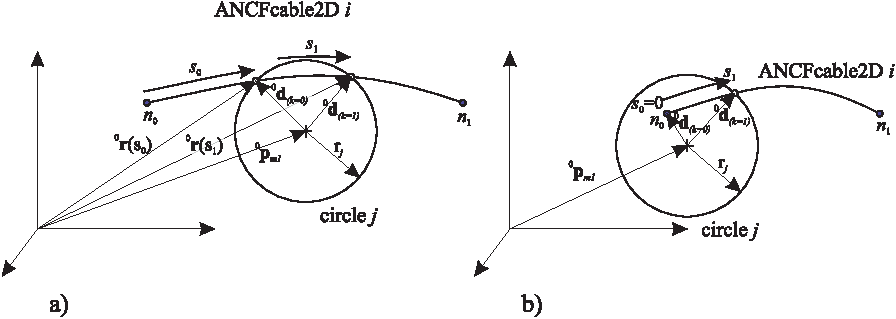
\includegraphics[width=\textwidth]{figures/generalContactANCF2Dcircle}
  \end{center}
  \caption{Geometrical relations for contact of ANCFCable2D $i$ and circle $j$ with according marker $m1$; case a) shows a cable with nodes $n_0$ and $n_1$, partially penetrating at the midspan of the cable; case b) shows the case of a cable where node $n_0$ is inside the cable.}
  \label{fig_generalContactANCF2Dcircle}
\end{figure}
%++++++++++++++++++++++++

Normal contact and tangential friction forces are then computed based on integrals over the coordinates $[s_0,\, s_1]$.
The integration is performed over $n_{ip}$ integration points $x_k \in [x_{i0},\, x_{i1},\, \ldots]$. In case of a 3 point Lobatto integration, we chose the integration points 
\be
  x_k \in [s_0, (s_0+s_1)/2, s_1] \eqDot
\ee
According weights are
\be
  w_k \in [1/3, 4/3, 1/3] \eqDot
\ee
The ANCF cable provides the global position of an integration point $k \in \{i0,\, i1,\, \ldots\}$ via
\be
  \LU{0}{\rv(x_{k})} = \LU{0}{\Sm(x_{k})} \qv
\ee
with ANCF shape function matrix $\Sm$ and current ANCF coordinates $\qv$.
Note that in the simplified case with linear segments, $\LU{0}{\rv(x_{k})}$ is computed from linear interpolation of the segment which is attached to the cable.
The velocity is computed in the same way,
\be
  \LU{0}{\dot \rv(x_{k})} = \LU{0}{\Sm(x_{k})} \dot\qv
\ee
again using linear interpolation of the velocities along the straight segment, if linear segments are used.

In order to perform the integration of contact forces due to penetration as well as tangential (friction) forces, we iterate over all integration points, and sum up the according generalized forces on the cable and the circle marker object.

\noindent The integration factor for integration point $k$ follows from
\be
  f_k = \frac{s_1 - s_0}{2} w_k \eqComma
\ee
assuming axial stretch of the cable element being moderately small.
The vector $\ANCFdk$ which points from the center of the circle to the cable (integration) point reads
\be
  \ANCFdk = \LU{0}{\rv(x_{k})} - \LU{0}{\pv_j} 
\ee
The velocity of the circle at the contact integration point $k$ follows as
\be
  \LU{0}{\vv_{c,k}} = \LU{0}{\vv_j} + \left( \LU{0,m0}{\Am} \LU{m0}{\tomega}_{j} \right) \times \ANCFdk
\ee
The distance $L$ between cable and circle center point, gap $g$ and the contact normal vector read
\be
  L_k = |\ANCFdk|, \quad g= L_k - (r + h_{1/2}), \quad \LU{0}{\dv_{0,k}} = \frac{1}{L_k} \ANCFdk
\ee
with the half height of the ANCF element $h_{1/2}$, which gives additional penetration. Note that this height is added on the side of the circle, which virtually represents a larger circle, behaving slightly different from a cable with thickness $h$.

\noindent The velocity in contact normal direction reads (note that we use the velocity of the circle's center point),
\be
  v_n = \LU{0}{\dv_{0,k}} \left( \LU{0}{\dot \rv(x_{k})} - \LU{0}{\vv}_j \right)
\ee
The contact force (tension! is always negative) follows in the simplistic case of a linear contact model as
\be \label{eq_GeneralContactASfc}
  f_{c,k} = k_c \cdot g  + d \cdot v_n
\ee
with contact stiffness $k_c$ and contact normal damping $d_c$.

\noindent In case of tangential friction, the tangential velocity reads
\bea
  \vv_{t,k} &=& \LU{0}{\dot \rv(x_{k})} - \LU{0}{\vv}_{c,k} - v_n \cdot \LU{0}{\dv_{0,k}}
  = \LU{0}{\dot \rv(x_{k})} - \LU{0}{\vv_j} - \left( \LU{0,m0}{\Am} \LU{m0}{\tomega}_{j} \right) \times \ANCFdk - v_n \cdot \LU{0}{\dv_{0,k}} \nonumber \\
  &=& -\left(\LU{0}{\dv_{0,k}} \otimes \LU{0}{\dv_{0,k}} -\Im \right) \left( \LU{0}{\dot \rv(x_{k})} - \LU{0}{\vv}_{c,k} \right) 
      +\LU{0}{\tilde \dv_k} \LU{0,m0}{\Am} \LU{m0}{\tomega}_{j} 
\eea
and the friction force is computed from \eq{eq_GeneralContactRegularizedFriction} using the contact pressure $-f_{c,k}$ from \eq{eq_GeneralContactASfc}, while otherwise $\LU{0}{\fv_f} = \Null$.

The force vector for the contact point for integration point $k$, including integration weight $f_k$\footnote{this is done, because all further terms are proportional to $\fv_k$.} thus reads
\be
  \LU{0}{\fv_k} = f_k \cdot \left(f_{c,k} \cdot \LU{0}{\dv_{0,k}} + \LU{0}{\fv_f} \right)
\ee
%
The total force and torque on the circle $j$ is found by summation over all integration points $k$,
\be
  \LU{0}{\fv_{circ}} = \sum_k \LU{0}{\fv_{circ,k}}  = \sum_k \LU{0}{\fv_k}, \quad
  \LU{0}{\tv_{circ}} = \sum_k \LU{0}{\tv_{circ,k}}  = \sum_k \left( r_j \cdot \LU{0}{\dv_{0,k}} \right) \times \LU{0}{\fv_k}
\ee
and the contribution to the generalized forces of the ANCF cable element (with generalized coordinates $\qv_{ANCF}$) read
\be
  \fv_{ANCF} = \sum_k \fv_{ANCF,k} = \sum_k \LU{0}{\Sm(x_{k})\tp} \cdot \LU{0}{\fv_k}
\ee
%Note that in the implementation, $f_k$ is already included in the contact force $\fv_k$.
%
The generalized \ac{LHS} forces for marker $m1$ (with generalized coordinates $\qv_{m1}$) thus read
\be
  \fv_{m1,LHS} = \LU{0}{\Jm_{pos,m1}\tp} \LU{0}{\fv_{circ}} + 
                 \LU{0}{\Jm_{rot,m1}\tp} \LU{0}{\tv_{circ}} \eqDot
\ee
The Jacobian matrix for the circle-ANCF contact on position level thus reads\footnote{terms that are implemented are marked in green; black terms are not implemented or unused},
\be
  \termA{
  \Jm_{c}  = \mp{\diffANCF{ \LU{0}{\fv_{ANCF}} }}
                {\diffmI{   \LU{0}{\fv_{ANCF}} }}
                {-\diffANCF{ \left( \LU{0}{\Jm_{pos,m1}\tp} \LU{0}{\fv_{circ}} + \LU{0}{\Jm_{rot,m1}\tp} \LU{0}{\tv_{circ}}\right)}}
                {\diffmI{ \left( \LU{0}{\Jm_{pos,m1}\tp} \LU{0}{\fv_{circ}} + \LU{0}{\Jm_{rot,m1}\tp} \LU{0}{\tv_{circ}}\right)}}
                }
\ee
and on velocity level, it follows as
\be
  \termA{
  \Jm_{c}  = \mp{\diffANCFt{ \LU{0}{\fv_{ANCF}} }}
                {\diffmIt{   \LU{0}{\fv_{ANCF}} }}
                {-\diffANCFt{ \left( \LU{0}{\Jm_{pos,m1}\tp} \LU{0}{\fv_{circ}} + \LU{0}{\Jm_{rot,m1}\tp} \LU{0}{\tv_{circ}}\right)}}
                {\diffmIt{ \left( \LU{0}{\Jm_{pos,m1}\tp} \LU{0}{\fv_{circ}} + \LU{0}{\Jm_{rot,m1}\tp} \LU{0}{\tv_{circ}}\right)}}
                }
\ee
For the calculation of the jacobian, the derivatives of the following terms are needed:
\bi
  \item $\ANCFdk = \LU{0}{\rv(x_{k})} - \LU{0}{\pv_j} $:
  \be
    \diffANCF{\ANCFdk} = \diffANCF{\LU{0}{\rv(x_{k})} - \LU{0}{\pv_j} }
    = \LU{0}{\Sm(x_{k})}
  \ee
  \be
    \diffmI{\ANCFdk} = \diffmI{\LU{0}{\rv(x_{k})} - \LU{0}{\pv_j} }
    = -\LU{0}{\Jm_{pos,m1}}
  \ee
  \item $\ANCFdkt = \LU{0}{\dot \rv(x_{k})} - \LU{0}{\dot \vv_j} $:
  \be
    \diffANCFt{\ANCFdkt} = \diffANCF{\LU{0}{\dot \rv(x_{k})} - \LU{0}{\vv_j} }
    = \LU{0}{\Sm(x_{k})}
  \ee
  \be
    \diffmIt{\ANCFdkt} = \diffmI{\LU{0}{\dot \rv(x_{k})} - \LU{0}{\vv_j} }
    = -\LU{0}{\Jm_{pos,m1}}
  \ee
  \item $L_k = |\ANCFdk| = \left(\LU{0}{\dv_k\tp} \ANCFdk \right) ^{1/2}$:
  \be
    \diffANCFmI{ |\ANCFdk| } = \frac{1}{L_k}\left(\LU{0}{\dv_k\tp} \diffANCFdk \right) =
    \ANCFdkOtp \diffANCFdk 
  \ee
  %\be
    %\diffmI{ |\ANCFdk| } = - \frac{1}{L_k}\left(\LU{0}{\dv_k\tp} \LU{0}{\Jm_{pos,m1}} \right) =
    %-\left(\ANCFdkO\!\tp \LU{0}{\Jm_{pos,m1}} \right) 
  %\ee
  \item $L_k^{-1} = \left(\LU{0}{\dv_k\tp} \ANCFdk \right) ^{-1/2}$ (note different sign as in $L$-term due to $-1/2$):
  \be
    \diffANCFmI{ L_k^{-1} } = \diffANCFmI{\left(\LU{0}{\dv_k\tp} \ANCFdk \right) ^{-1/2} } = 
    -\frac{1}{L_k}\left(\ANCFdkOtp \diffANCFdk \right)
  \ee
  %\be
    %\diffmI{ L_k^{-1} } = \diffmI{\left(\LU{0}{\dv_k\tp} \ANCFdk \right) ^{-1/2} } = 
    %\frac{1}{2\cdot L_k^3}\left(\LU{0}{\dv_k\tp} \LU{0}{\Jm_{pos,m1}} \right)
  %\ee
  %\item $L^{-1} = \left(\LU{0}{\nv}\!\tp\LU{0}{\nv}\right)^{-\frac{1}{2}}$:
  %\be
    %\termC{\frac{\partial L^{-1}}{\partial \qv_{m0}} =
    %\frac{\partial \left(\LU{0}{\nv}\!\tp\LU{0}{\nv}\right)^{-\frac{1}{2}} }{\partial \qv_{m0}} =
    %-\frac{1}{2\cdot L^3}\left(\LU{0}{\nv}\!\tp \frac{\partial \LU{0}{\nv}}{\partial \qv_{m0}} \right) =
    %\frac{1}{2\cdot L^3}\left(\LU{0}{\nv}\!\tp \LU{0}{\Jm_{pos,m0}} \right) }
  %\ee
  \item $\ANCFdkO = \frac{1}{L_k} \ANCFdk$: 
  \be
    \diffANCFmI{ \ANCFdkO } = \diffANCFmI{\frac{1}{L_k} \ANCFdk } = 
    - \frac{1}{L_k^2}\ANCFdk \otimes \left(\ANCFdkOtp \diffANCFdk \right) 
    + \frac{1}{L_k} \diffANCFdk = \frac{1}{L_k} \left(\Im - \ANCFdkO \otimes \ANCFdkO \right) \diffANCFdk
    \ee
  %\be
    %\diffmI{ \ANCFdkO } = \diffmI{\frac{1}{L_k} \ANCFdk } = 
      %\frac{1}{2\cdot L_k^3}\left(\LU{0}{\dv_k\tp} \LU{0}{\Jm_{pos,m1}} \right) \ANCFdk
    %- \frac{1}{L_k} \LU{0}{\Jm_{pos,m1}}
  %\ee
  \item $g= L_k - (r + h_{1/2})$:
  \be
    \diffANCFmI{ g } = \diffANCFmI{ L_k } =
    \ANCFdkOtp \diffANCFdk 
    %\LU{0}{\Sm(x_{k})}
  \ee
  %\be
    %\diffmI{ p } = -\frac{1}{L_k}\left(\ANCFdk\!\tp \LU{0}{\Jm_{pos,m1}} \right) =
    %-\ANCFdkO\!\tp \LU{0}{\Jm_{pos,m1}} 
  %\ee
  %+++++++++++++++++++++++++++++++++++++++++++++++++++++++++++++++++++++++++++++++++++++++++++++++++++++++++
  \item velocity at circle contact point $k$: $\LU{0}{\vv_{c,k}} = \LU{0}{\vv_j} + \left( \LU{0,m1}{\Am} \LU{m1}{\tomega}_{j} \right) \times \ANCFdk = \LU{0}{\vv_j} - \LU{0}{\tilde \dv_k} \LU{0,m1}{\Am} \LU{m1}{\tomega}_{j} $:
  \be
    \diffmIt{ \LU{0}{\vv_{c,k}} } =\LU{0}{\Jm_{pos,m1}}  - \LU{0}{\tilde \dv_k} \LU{0}{\Jm_{rot,m1}}
  \ee
  %+++++++++++++++++++++++++++++++++++++++++++++++++++++++++++++++++++++++++++++++++++++++++++++++++++++++++
  \item $v_n = \ANCFdkO \left( \LU{0}{\dot \rv(x_{k})} - \LU{0}{\vv}_{c,k} \right)$:\footnote{the approximate sign is used, because $\LU{0}{\vv}_{c,k}$ includes a normal component if ANCF cable is not fully tangential, which is not considered here.}
  \be
    \diffANCFmIt{ v_n } = \ANCFdkO \diffANCFt{\left( \LU{0}{\dot \rv(x_{k})} - \LU{0}{\vv}_{c,k} \right) } 
    \approx %because \LU{0}{\vv}_{c,k} includes normal component if ANCF cable is not fully tangential
        \ANCFdkOtp \diffANCFdk
  \ee
  %\be
    %\diffmIt{ v_n } = \ANCFdkO \diffmIt{\left( \LU{0}{\dot \rv(x_{k})} - \LU{0}{\vv}_{c,k} \right) } 
    %\approx -\ANCFdkO \LU{0}{\Jm_{pos,m1}}
  %\ee
  %+++++++++++++++++++++++++++++++++++++++++++++++++++++++++++++++++++++++++++++++++++++++++++++++++++++++++
  \item $\vv_{t,k} = \LU{0}{\dot \rv(x_{k})} - \LU{0}{\vv}_j - v_n \cdot \ANCFdkO =
  \left(\Im - \ANCFdkO \otimes \ANCFdkO \right) \left( \LU{0}{\dot \rv(x_{k})} - \LU{0}{\vv_j} \right) 
      +\LU{0}{\tilde \dv_k} \LU{0}{\tomega}_{j} $:
  \be
    \diffANCFt{\vv_{t,k} } = \left(\Im - \ANCFdkO \otimes \ANCFdkO \right) \LU{0}{\Sm(x_{k})}
  \ee
  \be
    \diffmIt{\vv_{t,k} } = -\left(\Im - \ANCFdkO \otimes \ANCFdkO \right) \LU{0}{\Jm_{pos,m1}} + \LU{0}{\tilde \dv_k} \LU{0}{\Jm_{rot,m1}}
  \ee
  %+++++++++++++++++++++++++++++++++++++++++++++++++++++++++++++++++++++++++++++++++++++++++++++++++++++++++
  \item $f_{c,k} = k_c \cdot g  + d_c \cdot v_n$:
  \be 
    \termA{ \diffANCF{ f_{c,k} } } = \termC{ k_c \cdot \diffANCF{ g } }  + d_c \cdot \diffANCF{ v_n }
    \approx \termC{ k_c \cdot \LU{0}{\dv_{k,0}\tp} \LU{0}{\Sm(x_{k})} }
  \ee
  \be 
    \termA{ \diffmI{ f_{c,k} } } = \termC{ k_c \cdot \diffmI{ p } }  + d_c \cdot \diffmI{ v_n }
    \approx \termC{ -k_c \cdot \LU{0}{\dv_{k,0}\tp} \LU{0}{\Jm_{pos,m1}} }
  \ee
  \be 
    \termC{\diffANCFt{ f_{c,k} } = d_c \cdot \diffANCFt{ v_n } = d_c \cdot \ANCFdkO \LU{0}{\Sm(x_{k})} }
  \ee  
  \be 
    \termC{\diffmIt{ f_{c,k} } = d_c \cdot \diffmIt{ v_n } = -d_c \cdot \ANCFdkO \LU{0}{\Jm_{pos,m1}} }
  \ee  
  %+++++++++++++++++++++++++++++++++++++++++++++++++++++++++++++++++++++++++++++++++++++++++++++++++++++++++
\ei
The contact force reads (note that because $f_c$ is always negative, the sign of regularization term is negative),
\be
  \LU{0}{\fv_k} = f_k \cdot \left( f_{c,k} \cdot \ANCFdkO + \fv_f \right)
                =
              \begin{cases}
                f_k \cdot f_{c,k} \left(\ANCFdkO - \frac{\mu_s}{v_{\mu,reg}}\LU{0}{\vv_t} \right), \quad \mathrm{if} \quad |\LU{0}{\vv_t}| < v_{\mu,reg} \\
                f_k \cdot \left( f_{c,k} \cdot \ANCFdkO + \fv_f \right), \quad \mbox{else with $\fv_f = const.$} 
              \end{cases}
\ee
%++++++++++++++++++++++++++
We introduce a factor $\delta_f$, which is $\delta_f=1$ in the regularized small velocity state, and in the saturated (constant) friction force we use $\delta_f=0$. Thus, the derivative of $\fv_f$, using $|f_{c,k}| = -f_{c,k}$, reads:
  \bea
    \termA{ \diffANCFmIt{\fv_f} } &=& \termA{ \delta_f \frac{\mu_s}{v_{\mu,reg}} \diffANCFmIt{ (-f_{c,k} \LU{0}{\vv_t}) } } \approx
    \termC{ -\delta_f f_{c,k} \frac{\mu_s}{v_{\mu,reg}} \diffANCFmIt{ \LU{0}{\vv_t} } } \nonumber \\
    \termC{ \diffANCFt{\fv_f} } &\approx& \termC{ -\delta_f f_{c,k} \frac{\mu_s}{v_{\mu,reg}} \left(\Im - \ANCFdkO \otimes \ANCFdkO \right) \LU{0}{\Sm(x_{k})} } \nonumber \\
    \termC{ \diffmIt{\fv_f} } &\approx& \termC{ -\delta_f f_{c,k} \frac{\mu_s}{v_{\mu,reg}} \left(-\left(\Im - \ANCFdkO \otimes \ANCFdkO \right) \LU{0}{\Jm_{pos,m1}} + \LU{0}{\tilde \dv_k} \LU{0}{\Jm_{rot,m1}} \right) }
    %+ \LU{0}{\tilde \dv_k} \LU{0}{\Jm_{rot,m1}} \right)
     %\mbox{??? minus in term 3 ???}
  \eea
%
%+++++++++++++++++++++++++++++++++++++++++++++++++++++++++++++++++++++++++++++++++++++++++++++++++++++++++
The term $\LU{0}{\fv_k}$ gives:
  \bea
    \termA{\frac{\partial \LU{0}{\fv_k}}{\partial \qv_{ANCF,m1}} } &=& 
    \termC{f_k \cdot} \left(\termA{ \left(\ANCFdkO - \frac{\mu_s}{v_{\mu,reg}}\LU{0}{\vv_t} \right) \otimes \frac{\partial f_{c,k}}{\partial \qv_{ANCF,m1}} } + 
    f_{c,k} \cdot \frac{\partial \ANCFdkO}{\partial \qv_{ANCF,m1}} +
    \diffANCFmI{\LU{0}{\fv_f}} \right)  \nonumber \\
    &\approx& \termC{f_k \cdot k_c \cdot \left( \left(\ANCFdkO - \frac{\mu_s}{v_{\mu,reg}}\LU{0}{\vv_t} \right) \otimes \ANCFdkO \diffANCFmI{\LU{0}{\dv_{k}}} \right) }
  \eea
and the velocity terms yield
  \bea
    \termA{\diffANCFt{\LU{0}{\fv_k}} } &=& 
    \termC{f_k \cdot \left(d_c \cdot \left(\ANCFdkO - \frac{\mu_s}{v_{\mu,reg}}\LU{0}{\vv_t} \right) \otimes \diffANCFt{v_n}  + 
    \diffANCFt{\LU{0}{\fv_f}} \right) } \nonumber \\
    &\approx& \termC{f_k \cdot \left( d_c \cdot \left(\ANCFdkO - \frac{\mu_s}{v_{\mu,reg}}\LU{0}{\vv_t} \right) \otimes \ANCFdkO -
    \delta_f f_{c,k} \frac{\mu_s}{v_{\mu,reg}} \left(\Im - \ANCFdkO \otimes \ANCFdkO \right) \right)\diffANCFt{\ANCFdkt}  }
  \eea
  \bea
    \termA{\diffmIt{\LU{0}{\fv_k}} } &=& 
    \termC{f_k \cdot \left(d_c \cdot \left(\ANCFdkO - \frac{\mu_s}{v_{\mu,reg}}\LU{0}{\vv_t} \right) \otimes \diffmIt{v_n}  + 
    \diffmIt{\LU{0}{\fv_f}} \right) } \nonumber \\
    &\approx& \termC{f_k \cdot \left( \left( d_c \cdot \left(\ANCFdkO - \frac{\mu_s}{v_{\mu,reg}}\LU{0}{\vv_t} \right) \otimes \ANCFdkO  -
    \delta_f f_{c,k} \frac{\mu_s}{v_{\mu,reg}} \left(\Im - \ANCFdkO \otimes \ANCFdkO\right) \right) \diffmIt{\ANCFdkt}\right.  } \nonumber\\
    && \termC{\left.  + \delta_f f_{c,k} \frac{\mu_s}{v_{\mu,reg}} \LU{0}{\tilde \dv_k} \LU{0}{\Jm_{rot,m1}} \right) }
  \eea
%++++++++++++++++++++++++++
%
The single jacobian terms w.r.t.\ $\qv_{ANCF}$ and $\qv_{m1}$ may be expressed as
%terms with $\diamond$ are neglected in the current implementation}
\bea
  &&\termA{\frac{\partial \left( \LU{0}{\Jm_{pos,m1}\tp} \LU{0}{\fv_{circ}} + \LU{0}{\Jm_{rot,m1}\tp} \LU{0}{\tv_{circ}}\right)}{\partial \qv_{ANCF,m1}}} = \nonumber \\
  &&\frac{\partial \LU{0}{\Jm_{pos,m1}\tp}}{\partial \qv_{ANCF,m1}} \LU{0}{\fv_{circ}}
  +\termC{\LU{0}{\Jm_{pos,m1}\tp}} \termA{\frac{\partial \LU{0}{\fv_{circ}}}{\partial \qv_{ANCF,m1}}}
  +\frac{\partial \LU{0}{\Jm_{rot,m1}\tp}}{\partial \qv_{m0,1}} \LU{0}{\tv_{circ}}
  +\termC{\LU{0}{\Jm_{rot,m1}\tp}} \termA{\frac{\partial \LU{0}{\tv_{circ}}}{\partial \qv_{ANCF,m1}}}
\eea
%\frac{\partial  }{\partial \qv_{ANCF,m1}}
Note that similar relations follow for the time derivatives $\frac{\partial}{\partial \dot \qv_{ANCF,m1}}\left( \right) $.

\noindent The derivatives of $\LU{0}{\fv_{ANCF}}$, $\LU{0}{\fv_{circ}}$, and 
\be
  \LU{0}{\tv_{circ}} = \sum_k r_j \cdot  \ANCFdkO \times \LU{0}{\fv_k} = 
                       \sum_k r_j \cdot  \LU{0}{\tilde \dv_{0,k}} \LU{0}{\fv_k}
\ee
follow from
%\LU{0}{\tv_{circ}} = \sum_k \LU{0}{\tv_{circ,k}}  = \sum_k \left( r_j \cdot \ANCFdkO \right) \times \cdot \LU{0}{\fv_k}
\bea
  \diffANCFmI{\LU{0}{\fv_{ANCF}} } &=& \termC{\sum_k \LU{0}{\Sm(x_{k})\tp}} \termA{\frac{\partial \LU{0}{\fv_k}}{\partial \qv_{ANCF,m1}}}, \nonumber \\
  %\termA{-\LU{0}{\Jm_{pos,m0}\tp} \frac{\partial  \LU{0}{\fv_{ANCF}} }{\partial \qv_{ANCF,m1}}}
  %\termA{\frac{\partial  \LU{0}{\fv_{ANCF}} }{\partial \qv_{ANCF,m1}}} &=& 
  %\termC{\sum_k \LU{0}{\Sm(x_{k})\tp}} \termA{\frac{\partial \LU{0}{\fv_k}}{\partial \qv_{ANCF,m1}}}, \nonumber \\
%
  \termA{\diffANCFmI{ \LU{0}{\fv_{circ}} } } &=& \termA{ \sum_k \diffANCFmI{ \LU{0}{\fv_k} } }, \nonumber \\
%
  \termA{\frac{\partial  \LU{0}{\tv_{circ}} }{\partial \qv_{ANCF,m1}}} &\approx& 
  \sum_k \left( \termC{r_j \cdot  \LU{0}{\tilde \dv_{0,k}} } \termA{\diffANCFmI{\LU{0}{\fv_k}} } - 
                r_j \cdot \LU{0}{\tilde \fv_k} \diffANCFmI{\LU{0}{\dv_{0,k}} } \right)
\eea


%+++++++++++++++++++++++++++++++++++++++++++++++++++++++++++++++++++++++++++++++++++++++++++++++++
    %\mysubsubsubsection{Connector forces}
    %%
    %The unit vector in force direction reads (raises SysError if $L=0$),
    %\be
      %\vv_{f} = \frac{1}{L} \Delta\! \LU{0}{\pv}
    %\ee
    %If \texttt{activeConnector = True}, the scalar spring force is computed as
    %\be
      %f_{SD} = k\cdot(L-L_0) + d \cdot\Delta\! \LU{0}{\vv}\tp \vv_{f} + f_{a}
    %\ee
    %If the springForceUserFunction $\mathrm{UF}$ is defined, $\fv$ instead becomes ($t$ is current time)
    %\be
      %f_{SD} = \mathrm{UF}(mbs, t, i_N, L-L_0, \Delta\! \LU{0}{\vv}\tp \vv_{f}, k, d, f_{a})
    %\ee
    %and \texttt{iN} represents the itemNumber (=objectNumber). Note that, if \texttt{activeConnector = False}, $f_{SD}$ is set to zero.
%
    %The vector of the spring-damper force applied at both markers finally reads
    %\be
      %\fv = f_{SD}\vv_{f}
    %\ee
    %The virtual work of the connector force is computed from the virtual displacement 
    %\be
      %\delta \Delta\! \LU{0}{\pv} = \delta \LU{0}{\pv}_{m1} - \delta \LU{0}{\pv}_{m0} \eqComma
    %\ee
    %and the virtual work (not the transposed version here, because the resulting generalized forces shall be a column vector,
    %\be
      %\delta W_{SD} = \fv \delta \Delta\! \LU{0}{\pv} 
      %= \left( k\cdot(L-L_0) + d \cdot\Delta\! \LU{0}{\vv}\tp \vv_{f} + f_{a} \right) \left(\delta \LU{0}{\pv}_{m1} - \delta \LU{0}{\pv}_{m0} \right)\tp \vv_{f} 
      %\eqDot
    %\ee
    %The generalized (elastic) forces thus result from
    %\be
      %\Qm_{SD} = \frac{\partial \LU{0}{\pv}}{\partial \qv_{SD}\tp} \fv 
      %\eqComma
    %\ee
    %and read for the markers $m0$ and $m1$,
    %\be
      %\Qm_{SD, m0} 
      %= -\left( k\cdot(L-L_0) + d \cdot\Delta\! \LU{0}{\vv}\tp \vv_{f} + f_{a} \right) \Jm_{pos,m0}\tp \vv_{f} , \quad
      %\Qm_{SD, m1} 
      %= \left( k\cdot(L-L_0) + d \cdot\Delta\! \LU{0}{\vv}\tp \vv_{f} + f_{a} \right) \Jm_{pos,m1}\tp \vv_{f} 
      %\eqComma    
    %\ee
    %where $\Jm_{pos,m1}$ represents the derivative of marker $m1$ w.r.t.\ its associated coordinates $\qv_{m1}$, analogously $\Jm_{pos,m0}$.
    %%
    %\mysubsubsubsection{Connector Jacobian}
    %The position-level jacobian for the connector, involving all coordinates associated with markers $m0$ and $m1$, follows from 
    %\be
      %\Jm_{SD} = \mp{\frac{\partial \Qm_{SD, m0}}{\partial \qv_{m0}} }{\frac{\partial \Qm_{SD, m0}}{\partial \qv_{m1}}}
                    %{\frac{\partial \Qm_{SD, m0}}{\partial \qv_{m1}} }{\frac{\partial \Qm_{SD, m1}}{\partial \qv_{m1}}}
    %\ee
    %and the velocity level jacobian reads
    %\be
      %\Jm_{SD,t} = \mp{\frac{\partial \Qm_{SD, m0}}{\partial \dot \qv_{m0}} }{\frac{\partial \Qm_{SD, m0}}{\partial \dot \qv_{m1}}}
                    %{\frac{\partial \Qm_{SD, m0}}{\partial \dot \qv_{m1}} }{\frac{\partial \Qm_{SD, m1}}{\partial \dot \qv_{m1}}}
    %\ee
    %The sub-Jacobians follow from
    %\be
      %\frac{\partial \Qm_{SD, m0}}{\partial \qv_{m0}} = 
       %-\frac{\partial \Jm_{pos,m0}\tp }{\partial \qv_{m0}} \vv_{f} \left( k\cdot(L-L_0) + d \cdot\Delta\! \LU{0}{\vv}\tp \vv_{f} + f_{a} \right) 
       %-\Jm_{pos,m0}\tp \frac{\partial \vv_{f} \left( k\cdot(L-L_0) + d \cdot\Delta\! \LU{0}{\vv}\tp \vv_{f} + f_{a} \right)   }{\partial \qv_{m0}} 
    %\ee
    %in which the term $\frac{\partial \Jm_{pos,m0}\tp }{\partial \dot \qv_{m0}}$ is computed from a special function provided by markers, that
    %compute the derivative of the marker jacobian times a constant vector, in this case the spring force $\fv$; this jacobian term is usually less  
    %dominant, but is included in the numerical as well as the analytical derivatives, see the general jacobian computation information.
    %
    %The other term, which is the dominant term, is computed as (dependence of velocity term on position coordinates neglected),
    %\bea
      %\frac{\partial \Qm_{SD, m0}}{\partial \qv_{m0}}
      %&=& -\Jm_{pos,m0}\tp \frac{\partial \vv_{f} \left( k\cdot(L-L_0) + d \cdot\Delta\! \LU{0}{\vv}\tp \vv_{f} + f_{a} \right)   }{\partial \qv_{m0}}
      %\nonumber \\
      %&=& -\Jm_{pos,m0}\tp \frac{\partial  \left( k\cdot \left( \Delta\! \LU{0}{\pv} - L_0 \vv_{f} \right)+ \vv_{f} \left(d \cdot \vv_{f}\tp \Delta\! \LU{0}{\vv}  + f_{a} \right) \right)   }{\partial \qv_{m0}} 
      %\nonumber \\
      %&\approx& \Jm_{pos,m0}\tp \left(k\cdot \Im - k  \frac{L_0}{L}\left(\Im - \LU{0}{\vv_{f}} \otimes \LU{0}{\vv_{f}} \right)  +\frac{1}{L}\left(\Im - \LU{0}{\vv_{f}} \otimes \LU{0}{\vv_{f}} \right) \left(d \cdot \vv_{f}\tp \Delta\! \LU{0}{\vv}  + f_{a} \right) \right)
      %\LU{0}{\Jm_{pos,m0}}
    %\eea
    %Noting that $\frac{\partial \vv_{f} }{\partial \qv_{m0}} = 
    %-\frac{1}{L}\left(\Im - \LU{0}{\vv_{f}} \otimes \LU{0}{\vv_{f}} \right) \LU{0}{\Jm_{pos,m0}}$ and 
    %$\frac{\partial \vv_{f} }{\partial \qv_{m1}} = 
    %\frac{1}{L}\left(\Im - \LU{0}{\vv_{f}} \otimes \LU{0}{\vv_{f}} \right) \LU{0}{\Jm_{pos,m1}}$.
%%
    %The Jacobian w.r.t.\ velocity coordinates follows as
    %\bea
      %\frac{\partial \Qm_{SD, m0}}{\partial \dot \qv_{m0}}
      %&=& -\Jm_{pos,m0}\tp \frac{\partial \vv_{f} \left( k\cdot(L-L_0) + d \cdot\Delta\! \LU{0}{\vv}\tp \vv_{f} + f_{a} \right)   }{\partial \dot \qv_{m0}}
      %\nonumber \\
      %&=& \Jm_{pos,m0}\tp \left(d \vv_{f} \otimes \vv_{f} \right) \LU{0}{\Jm_{pos,m0}} 
    %\eea
    %Jacobians for markers $m1$ and mixed $m0$/$m1$ terms follow analogously.
    
